\documentclass[twoside]{book}

% Packages required by doxygen
\usepackage{fixltx2e}
\usepackage{calc}
\usepackage{doxygen}
\usepackage[export]{adjustbox} % also loads graphicx
\usepackage{graphicx}
\usepackage[utf8]{inputenc}
\usepackage{makeidx}
\usepackage{multicol}
\usepackage{multirow}
\PassOptionsToPackage{warn}{textcomp}
\usepackage{textcomp}
\usepackage[nointegrals]{wasysym}
\usepackage[table]{xcolor}

% NLS support packages
\usepackage{polski}
\usepackage[T1]{fontenc}

% Font selection
\usepackage[T1]{fontenc}
\usepackage[scaled=.90]{helvet}
\usepackage{courier}
\usepackage{amssymb}
\usepackage{sectsty}
\renewcommand{\familydefault}{\sfdefault}
\allsectionsfont{%
  \fontseries{bc}\selectfont%
  \color{darkgray}%
}
\renewcommand{\DoxyLabelFont}{%
  \fontseries{bc}\selectfont%
  \color{darkgray}%
}
\newcommand{\+}{\discretionary{\mbox{\scriptsize$\hookleftarrow$}}{}{}}

% Page & text layout
\usepackage{geometry}
\geometry{%
  a4paper,%
  top=2.5cm,%
  bottom=2.5cm,%
  left=2.5cm,%
  right=2.5cm%
}
\tolerance=750
\hfuzz=15pt
\hbadness=750
\setlength{\emergencystretch}{15pt}
\setlength{\parindent}{0cm}
\setlength{\parskip}{3ex plus 2ex minus 2ex}
\makeatletter
\renewcommand{\paragraph}{%
  \@startsection{paragraph}{4}{0ex}{-1.0ex}{1.0ex}{%
    \normalfont\normalsize\bfseries\SS@parafont%
  }%
}
\renewcommand{\subparagraph}{%
  \@startsection{subparagraph}{5}{0ex}{-1.0ex}{1.0ex}{%
    \normalfont\normalsize\bfseries\SS@subparafont%
  }%
}
\makeatother

% Headers & footers
\usepackage{fancyhdr}
\pagestyle{fancyplain}
\fancyhead[LE]{\fancyplain{}{\bfseries\thepage}}
\fancyhead[CE]{\fancyplain{}{}}
\fancyhead[RE]{\fancyplain{}{\bfseries\leftmark}}
\fancyhead[LO]{\fancyplain{}{\bfseries\rightmark}}
\fancyhead[CO]{\fancyplain{}{}}
\fancyhead[RO]{\fancyplain{}{\bfseries\thepage}}
\fancyfoot[LE]{\fancyplain{}{}}
\fancyfoot[CE]{\fancyplain{}{}}
\fancyfoot[RE]{\fancyplain{}{\bfseries\scriptsize Wygenerowano przez Doxygen }}
\fancyfoot[LO]{\fancyplain{}{\bfseries\scriptsize Wygenerowano przez Doxygen }}
\fancyfoot[CO]{\fancyplain{}{}}
\fancyfoot[RO]{\fancyplain{}{}}
\renewcommand{\footrulewidth}{0.4pt}
\renewcommand{\chaptermark}[1]{%
  \markboth{#1}{}%
}
\renewcommand{\sectionmark}[1]{%
  \markright{\thesection\ #1}%
}

% Indices & bibliography
\usepackage{natbib}
\usepackage[titles]{tocloft}
\setcounter{tocdepth}{3}
\setcounter{secnumdepth}{5}
\makeindex

% Hyperlinks (required, but should be loaded last)
\usepackage{ifpdf}
\ifpdf
  \usepackage[pdftex,pagebackref=true]{hyperref}
\else
  \usepackage[ps2pdf,pagebackref=true]{hyperref}
\fi
\hypersetup{%
  colorlinks=true,%
  linkcolor=blue,%
  citecolor=blue,%
  unicode%
}

% Custom commands
\newcommand{\clearemptydoublepage}{%
  \newpage{\pagestyle{empty}\cleardoublepage}%
}

\usepackage{caption}
\captionsetup{labelsep=space,justification=centering,font={bf},singlelinecheck=off,skip=4pt,position=top}

%===== C O N T E N T S =====

\begin{document}

% Titlepage & ToC
\hypersetup{pageanchor=false,
             bookmarksnumbered=true,
             pdfencoding=unicode
            }
\pagenumbering{alph}
\begin{titlepage}
\vspace*{7cm}
\begin{center}%
{\Large Worms 2D \\[1ex]\large 1.\+0 }\\
\vspace*{1cm}
{\large Wygenerowano przez Doxygen 1.8.14}\\
\end{center}
\end{titlepage}
\clearemptydoublepage
\pagenumbering{roman}
\tableofcontents
\clearemptydoublepage
\pagenumbering{arabic}
\hypersetup{pageanchor=true}

%--- Begin generated contents ---
\chapter{Indeks hierarchiczny}
\section{Hierarchia klas}
Ta lista dziedziczenia posortowana jest z grubsza, choć nie całkowicie, alfabetycznie\+:\begin{DoxyCompactList}
\item Drawable\begin{DoxyCompactList}
\item \contentsline{section}{Bullet}{\pageref{class_bullet}}{}
\item \contentsline{section}{Button}{\pageref{class_button}}{}
\item \contentsline{section}{Menu}{\pageref{class_menu}}{}
\item \contentsline{section}{Terrain}{\pageref{class_terrain}}{}
\item \contentsline{section}{Water}{\pageref{class_water}}{}
\item \contentsline{section}{Weapon}{\pageref{class_weapon}}{}
\begin{DoxyCompactList}
\item \contentsline{section}{Bazooka}{\pageref{class_bazooka}}{}
\item \contentsline{section}{Revolver}{\pageref{class_revolver}}{}
\end{DoxyCompactList}
\item \contentsline{section}{Worm}{\pageref{class_worm}}{}
\end{DoxyCompactList}
\item \contentsline{section}{F\+P\+S\+Counter}{\pageref{class_f_p_s_counter}}{}
\item \contentsline{section}{Game\+Event}{\pageref{class_game_event}}{}
\item \contentsline{section}{Game\+Sound}{\pageref{class_game_sound}}{}
\item \contentsline{section}{Game\+Window}{\pageref{class_game_window}}{}
\end{DoxyCompactList}

\chapter{Indeks klas}
\section{Lista klas}
Tutaj znajdują się klasy, struktury, unie i interfejsy wraz z ich krótkimi opisami\+:\begin{DoxyCompactList}
\item\contentsline{section}{\mbox{\hyperlink{class_bazooka}{Bazooka}} }{\pageref{class_bazooka}}{}
\item\contentsline{section}{\mbox{\hyperlink{class_bullet}{Bullet}} }{\pageref{class_bullet}}{}
\item\contentsline{section}{\mbox{\hyperlink{class_button}{Button}} }{\pageref{class_button}}{}
\item\contentsline{section}{\mbox{\hyperlink{class_f_p_s_counter}{F\+P\+S\+Counter}} }{\pageref{class_f_p_s_counter}}{}
\item\contentsline{section}{\mbox{\hyperlink{class_game_event}{Game\+Event}} }{\pageref{class_game_event}}{}
\item\contentsline{section}{\mbox{\hyperlink{class_game_sound}{Game\+Sound}} }{\pageref{class_game_sound}}{}
\item\contentsline{section}{\mbox{\hyperlink{class_game_window}{Game\+Window}} }{\pageref{class_game_window}}{}
\item\contentsline{section}{\mbox{\hyperlink{class_menu}{Menu}} }{\pageref{class_menu}}{}
\item\contentsline{section}{\mbox{\hyperlink{class_revolver}{Revolver}} }{\pageref{class_revolver}}{}
\item\contentsline{section}{\mbox{\hyperlink{class_terrain}{Terrain}} }{\pageref{class_terrain}}{}
\item\contentsline{section}{\mbox{\hyperlink{class_water}{Water}} }{\pageref{class_water}}{}
\item\contentsline{section}{\mbox{\hyperlink{class_weapon}{Weapon}} \\*Klasa bazowa broni }{\pageref{class_weapon}}{}
\item\contentsline{section}{\mbox{\hyperlink{class_worm}{Worm}} \\*Klasa worma (gracza) }{\pageref{class_worm}}{}
\end{DoxyCompactList}

\chapter{Indeks plików}
\section{Lista plików}
Tutaj znajduje się lista wszystkich plików z ich krótkimi opisami\+:\begin{DoxyCompactList}
\item\contentsline{section}{D\+:/\+Projekty/\+C++/\+Programowanie w C2/\+Worms 2\+D/\+Worms 2\+D/\mbox{\hyperlink{_bazooka_8cpp}{Bazooka.\+cpp}} }{\pageref{_bazooka_8cpp}}{}
\item\contentsline{section}{D\+:/\+Projekty/\+C++/\+Programowanie w C2/\+Worms 2\+D/\+Worms 2\+D/\mbox{\hyperlink{_bazooka_8h}{Bazooka.\+h}} }{\pageref{_bazooka_8h}}{}
\item\contentsline{section}{D\+:/\+Projekty/\+C++/\+Programowanie w C2/\+Worms 2\+D/\+Worms 2\+D/\mbox{\hyperlink{_bullet_8cpp}{Bullet.\+cpp}} }{\pageref{_bullet_8cpp}}{}
\item\contentsline{section}{D\+:/\+Projekty/\+C++/\+Programowanie w C2/\+Worms 2\+D/\+Worms 2\+D/\mbox{\hyperlink{_bullet_8h}{Bullet.\+h}} }{\pageref{_bullet_8h}}{}
\item\contentsline{section}{D\+:/\+Projekty/\+C++/\+Programowanie w C2/\+Worms 2\+D/\+Worms 2\+D/\mbox{\hyperlink{_button_8cpp}{Button.\+cpp}} }{\pageref{_button_8cpp}}{}
\item\contentsline{section}{D\+:/\+Projekty/\+C++/\+Programowanie w C2/\+Worms 2\+D/\+Worms 2\+D/\mbox{\hyperlink{_button_8h}{Button.\+h}} }{\pageref{_button_8h}}{}
\item\contentsline{section}{D\+:/\+Projekty/\+C++/\+Programowanie w C2/\+Worms 2\+D/\+Worms 2\+D/\mbox{\hyperlink{_f_p_s_counter_8cpp}{F\+P\+S\+Counter.\+cpp}} }{\pageref{_f_p_s_counter_8cpp}}{}
\item\contentsline{section}{D\+:/\+Projekty/\+C++/\+Programowanie w C2/\+Worms 2\+D/\+Worms 2\+D/\mbox{\hyperlink{_f_p_s_counter_8h}{F\+P\+S\+Counter.\+h}} }{\pageref{_f_p_s_counter_8h}}{}
\item\contentsline{section}{D\+:/\+Projekty/\+C++/\+Programowanie w C2/\+Worms 2\+D/\+Worms 2\+D/\mbox{\hyperlink{_game_event_8cpp}{Game\+Event.\+cpp}} }{\pageref{_game_event_8cpp}}{}
\item\contentsline{section}{D\+:/\+Projekty/\+C++/\+Programowanie w C2/\+Worms 2\+D/\+Worms 2\+D/\mbox{\hyperlink{_game_event_8h}{Game\+Event.\+h}} }{\pageref{_game_event_8h}}{}
\item\contentsline{section}{D\+:/\+Projekty/\+C++/\+Programowanie w C2/\+Worms 2\+D/\+Worms 2\+D/\mbox{\hyperlink{_game_sound_8cpp}{Game\+Sound.\+cpp}} }{\pageref{_game_sound_8cpp}}{}
\item\contentsline{section}{D\+:/\+Projekty/\+C++/\+Programowanie w C2/\+Worms 2\+D/\+Worms 2\+D/\mbox{\hyperlink{_game_sound_8h}{Game\+Sound.\+h}} }{\pageref{_game_sound_8h}}{}
\item\contentsline{section}{D\+:/\+Projekty/\+C++/\+Programowanie w C2/\+Worms 2\+D/\+Worms 2\+D/\mbox{\hyperlink{_game_window_8cpp}{Game\+Window.\+cpp}} }{\pageref{_game_window_8cpp}}{}
\item\contentsline{section}{D\+:/\+Projekty/\+C++/\+Programowanie w C2/\+Worms 2\+D/\+Worms 2\+D/\mbox{\hyperlink{_game_window_8h}{Game\+Window.\+h}} }{\pageref{_game_window_8h}}{}
\item\contentsline{section}{D\+:/\+Projekty/\+C++/\+Programowanie w C2/\+Worms 2\+D/\+Worms 2\+D/\mbox{\hyperlink{_menu_8cpp}{Menu.\+cpp}} }{\pageref{_menu_8cpp}}{}
\item\contentsline{section}{D\+:/\+Projekty/\+C++/\+Programowanie w C2/\+Worms 2\+D/\+Worms 2\+D/\mbox{\hyperlink{_menu_8h}{Menu.\+h}} }{\pageref{_menu_8h}}{}
\item\contentsline{section}{D\+:/\+Projekty/\+C++/\+Programowanie w C2/\+Worms 2\+D/\+Worms 2\+D/\mbox{\hyperlink{_revolver_8cpp}{Revolver.\+cpp}} }{\pageref{_revolver_8cpp}}{}
\item\contentsline{section}{D\+:/\+Projekty/\+C++/\+Programowanie w C2/\+Worms 2\+D/\+Worms 2\+D/\mbox{\hyperlink{_revolver_8h}{Revolver.\+h}} }{\pageref{_revolver_8h}}{}
\item\contentsline{section}{D\+:/\+Projekty/\+C++/\+Programowanie w C2/\+Worms 2\+D/\+Worms 2\+D/\mbox{\hyperlink{_source_8cpp}{Source.\+cpp}} }{\pageref{_source_8cpp}}{}
\item\contentsline{section}{D\+:/\+Projekty/\+C++/\+Programowanie w C2/\+Worms 2\+D/\+Worms 2\+D/\mbox{\hyperlink{_terrain_8cpp}{Terrain.\+cpp}} }{\pageref{_terrain_8cpp}}{}
\item\contentsline{section}{D\+:/\+Projekty/\+C++/\+Programowanie w C2/\+Worms 2\+D/\+Worms 2\+D/\mbox{\hyperlink{_terrain_8h}{Terrain.\+h}} }{\pageref{_terrain_8h}}{}
\item\contentsline{section}{D\+:/\+Projekty/\+C++/\+Programowanie w C2/\+Worms 2\+D/\+Worms 2\+D/\mbox{\hyperlink{_water_8cpp}{Water.\+cpp}} }{\pageref{_water_8cpp}}{}
\item\contentsline{section}{D\+:/\+Projekty/\+C++/\+Programowanie w C2/\+Worms 2\+D/\+Worms 2\+D/\mbox{\hyperlink{_water_8h}{Water.\+h}} }{\pageref{_water_8h}}{}
\item\contentsline{section}{D\+:/\+Projekty/\+C++/\+Programowanie w C2/\+Worms 2\+D/\+Worms 2\+D/\mbox{\hyperlink{_weapon_8cpp}{Weapon.\+cpp}} }{\pageref{_weapon_8cpp}}{}
\item\contentsline{section}{D\+:/\+Projekty/\+C++/\+Programowanie w C2/\+Worms 2\+D/\+Worms 2\+D/\mbox{\hyperlink{_weapon_8h}{Weapon.\+h}} }{\pageref{_weapon_8h}}{}
\item\contentsline{section}{D\+:/\+Projekty/\+C++/\+Programowanie w C2/\+Worms 2\+D/\+Worms 2\+D/\mbox{\hyperlink{_worm_8cpp}{Worm.\+cpp}} }{\pageref{_worm_8cpp}}{}
\item\contentsline{section}{D\+:/\+Projekty/\+C++/\+Programowanie w C2/\+Worms 2\+D/\+Worms 2\+D/\mbox{\hyperlink{_worm_8h}{Worm.\+h}} }{\pageref{_worm_8h}}{}
\end{DoxyCompactList}

\chapter{Dokumentacja klas}
\hypertarget{class_bazooka}{}\section{Dokumentacja klasy Bazooka}
\label{class_bazooka}\index{Bazooka@{Bazooka}}


Klasa bazooki.  




{\ttfamily \#include $<$Bazooka.\+h$>$}

Diagram dziedziczenia dla Bazooka\begin{figure}[H]
\begin{center}
\leavevmode
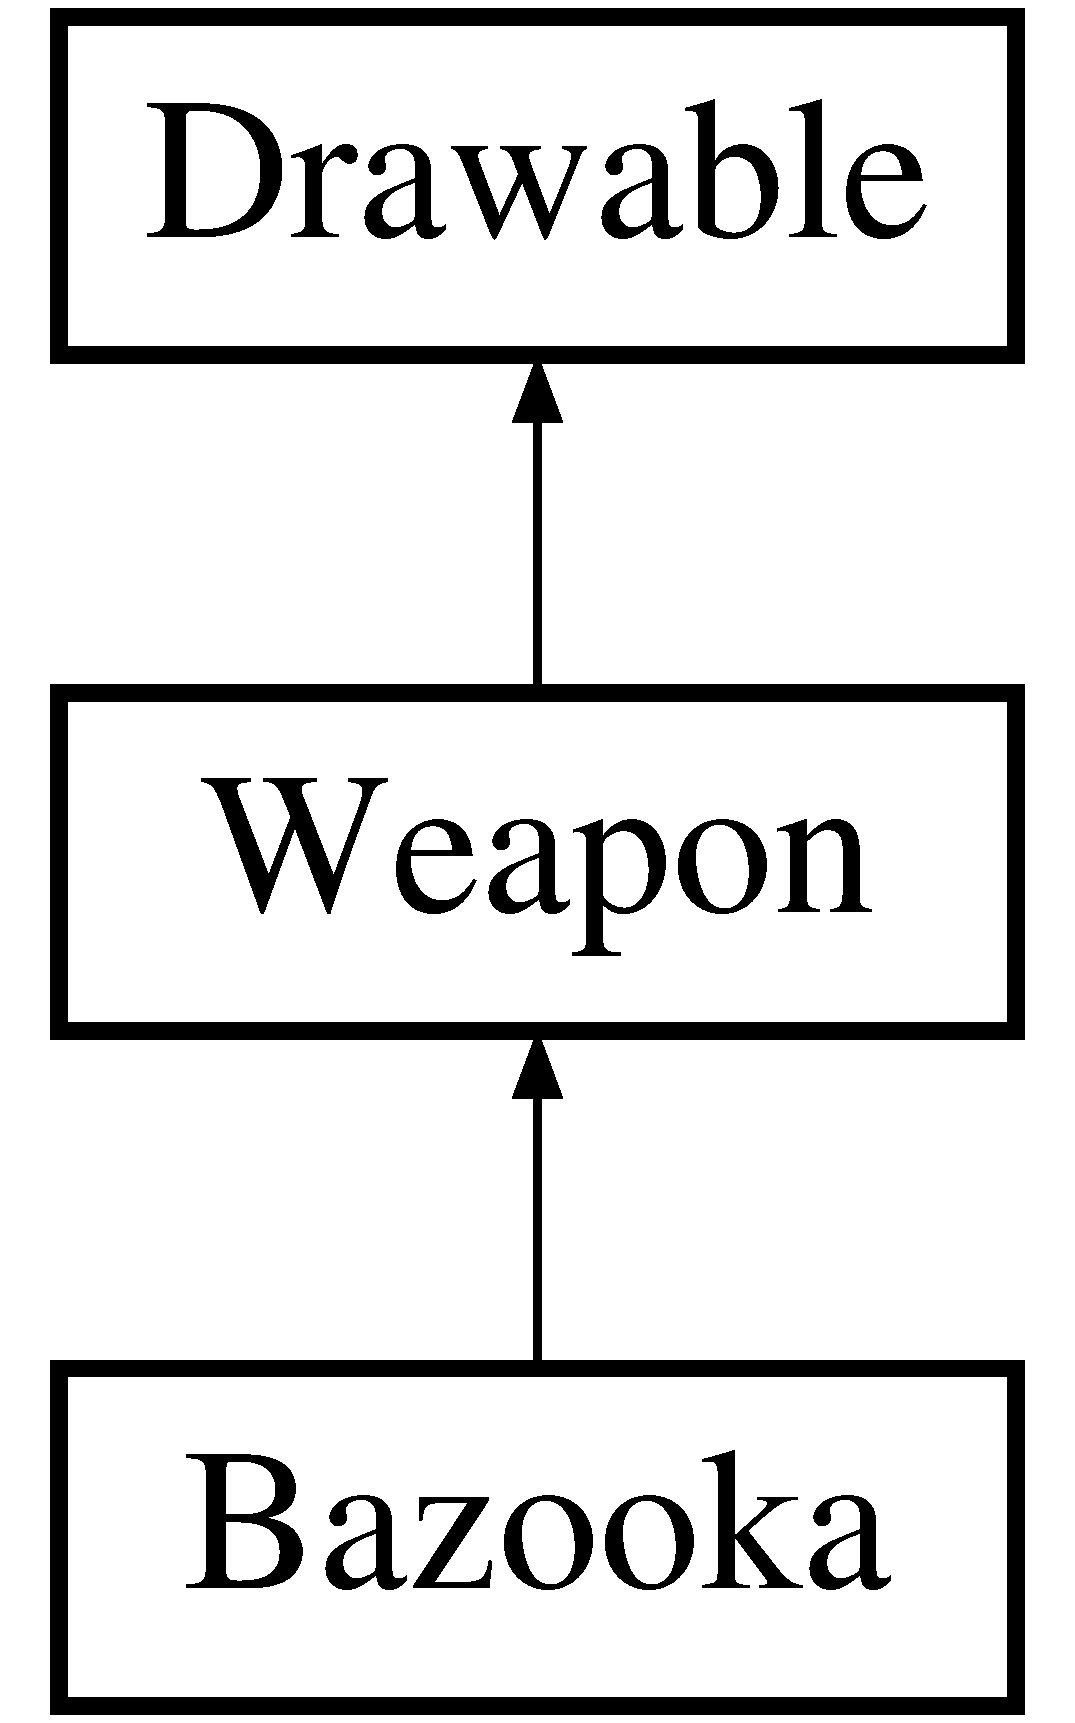
\includegraphics[height=3.000000cm]{class_bazooka}
\end{center}
\end{figure}
\subsection*{Metody publiczne}
\begin{DoxyCompactItemize}
\item 
\mbox{\hyperlink{class_bazooka_ab95ef6e55a5d1a7748df7287b562002b}{Bazooka}} ()=delete
\begin{DoxyCompactList}\small\item\em Konstruktor domyślny który jest usunięty. \end{DoxyCompactList}\item 
\mbox{\hyperlink{class_bazooka_aa3a6371f52b0649a6789401b8a11e8bd}{Bazooka}} (float x, float y)
\begin{DoxyCompactList}\small\item\em Konstruktor broni. \end{DoxyCompactList}\item 
virtual \mbox{\hyperlink{class_bazooka_a25ec2ef6a925a3b13947ad877d2ac823}{$\sim$\+Bazooka}} ()=default
\begin{DoxyCompactList}\small\item\em Domyślny destruktor. \end{DoxyCompactList}\item 
void \mbox{\hyperlink{class_bazooka_a2645b8043766ec5045e82d452828acdd}{play\+Shoot\+Sound}} () override
\begin{DoxyCompactList}\small\item\em Przeciążona funkcja odtwarzająca odgłos wystrzału z broni. \end{DoxyCompactList}\end{DoxyCompactItemize}
\subsection*{Dodatkowe Dziedziczone Składowe}


\subsection{Opis szczegółowy}
Klasa bazooki. 

Definicja w linii 7 pliku Bazooka.\+h.



\subsection{Dokumentacja konstruktora i destruktora}
\mbox{\Hypertarget{class_bazooka_ab95ef6e55a5d1a7748df7287b562002b}\label{class_bazooka_ab95ef6e55a5d1a7748df7287b562002b}} 
\index{Bazooka@{Bazooka}!Bazooka@{Bazooka}}
\index{Bazooka@{Bazooka}!Bazooka@{Bazooka}}
\subsubsection{\texorpdfstring{Bazooka()}{Bazooka()}\hspace{0.1cm}{\footnotesize\ttfamily [1/2]}}
{\footnotesize\ttfamily Bazooka\+::\+Bazooka (\begin{DoxyParamCaption}{ }\end{DoxyParamCaption})\hspace{0.3cm}{\ttfamily [delete]}}



Konstruktor domyślny który jest usunięty. 

\mbox{\Hypertarget{class_bazooka_aa3a6371f52b0649a6789401b8a11e8bd}\label{class_bazooka_aa3a6371f52b0649a6789401b8a11e8bd}} 
\index{Bazooka@{Bazooka}!Bazooka@{Bazooka}}
\index{Bazooka@{Bazooka}!Bazooka@{Bazooka}}
\subsubsection{\texorpdfstring{Bazooka()}{Bazooka()}\hspace{0.1cm}{\footnotesize\ttfamily [2/2]}}
{\footnotesize\ttfamily Bazooka\+::\+Bazooka (\begin{DoxyParamCaption}\item[{float}]{x,  }\item[{float}]{y }\end{DoxyParamCaption})}



Konstruktor broni. 


\begin{DoxyParams}{Parametry}
{\em x} & -\/ współrzędna x wyświetlenia miejsca broni \\
\hline
{\em y} & -\/ współrzędna y wyświetlenia miejsca broni \\
\hline
\end{DoxyParams}


Definicja w linii 4 pliku Bazooka.\+cpp.

\mbox{\Hypertarget{class_bazooka_a25ec2ef6a925a3b13947ad877d2ac823}\label{class_bazooka_a25ec2ef6a925a3b13947ad877d2ac823}} 
\index{Bazooka@{Bazooka}!````~Bazooka@{$\sim$\+Bazooka}}
\index{````~Bazooka@{$\sim$\+Bazooka}!Bazooka@{Bazooka}}
\subsubsection{\texorpdfstring{$\sim$\+Bazooka()}{~Bazooka()}}
{\footnotesize\ttfamily virtual Bazooka\+::$\sim$\+Bazooka (\begin{DoxyParamCaption}{ }\end{DoxyParamCaption})\hspace{0.3cm}{\ttfamily [virtual]}, {\ttfamily [default]}}



Domyślny destruktor. 



\subsection{Dokumentacja funkcji składowych}
\mbox{\Hypertarget{class_bazooka_a2645b8043766ec5045e82d452828acdd}\label{class_bazooka_a2645b8043766ec5045e82d452828acdd}} 
\index{Bazooka@{Bazooka}!play\+Shoot\+Sound@{play\+Shoot\+Sound}}
\index{play\+Shoot\+Sound@{play\+Shoot\+Sound}!Bazooka@{Bazooka}}
\subsubsection{\texorpdfstring{play\+Shoot\+Sound()}{playShootSound()}}
{\footnotesize\ttfamily void Bazooka\+::play\+Shoot\+Sound (\begin{DoxyParamCaption}{ }\end{DoxyParamCaption})\hspace{0.3cm}{\ttfamily [override]}, {\ttfamily [virtual]}}



Przeciążona funkcja odtwarzająca odgłos wystrzału z broni. 



Reimplementowana z \mbox{\hyperlink{class_weapon_aaf32c85f3e70d3c8392c928b9e6e75ca}{Weapon}}.



Definicja w linii 17 pliku Bazooka.\+cpp.



Dokumentacja dla tej klasy została wygenerowana z plików\+:\begin{DoxyCompactItemize}
\item 
D\+:/\+Projekty/\+C++/\+Programowanie w C2/\+Worms 2\+D/\+Worms 2\+D/\mbox{\hyperlink{_bazooka_8h}{Bazooka.\+h}}\item 
D\+:/\+Projekty/\+C++/\+Programowanie w C2/\+Worms 2\+D/\+Worms 2\+D/\mbox{\hyperlink{_bazooka_8cpp}{Bazooka.\+cpp}}\end{DoxyCompactItemize}

\hypertarget{class_bullet}{}\section{Dokumentacja klasy Bullet}
\label{class_bullet}\index{Bullet@{Bullet}}


Klasa pocisku.  




{\ttfamily \#include $<$Bullet.\+h$>$}

Diagram dziedziczenia dla Bullet\begin{figure}[H]
\begin{center}
\leavevmode
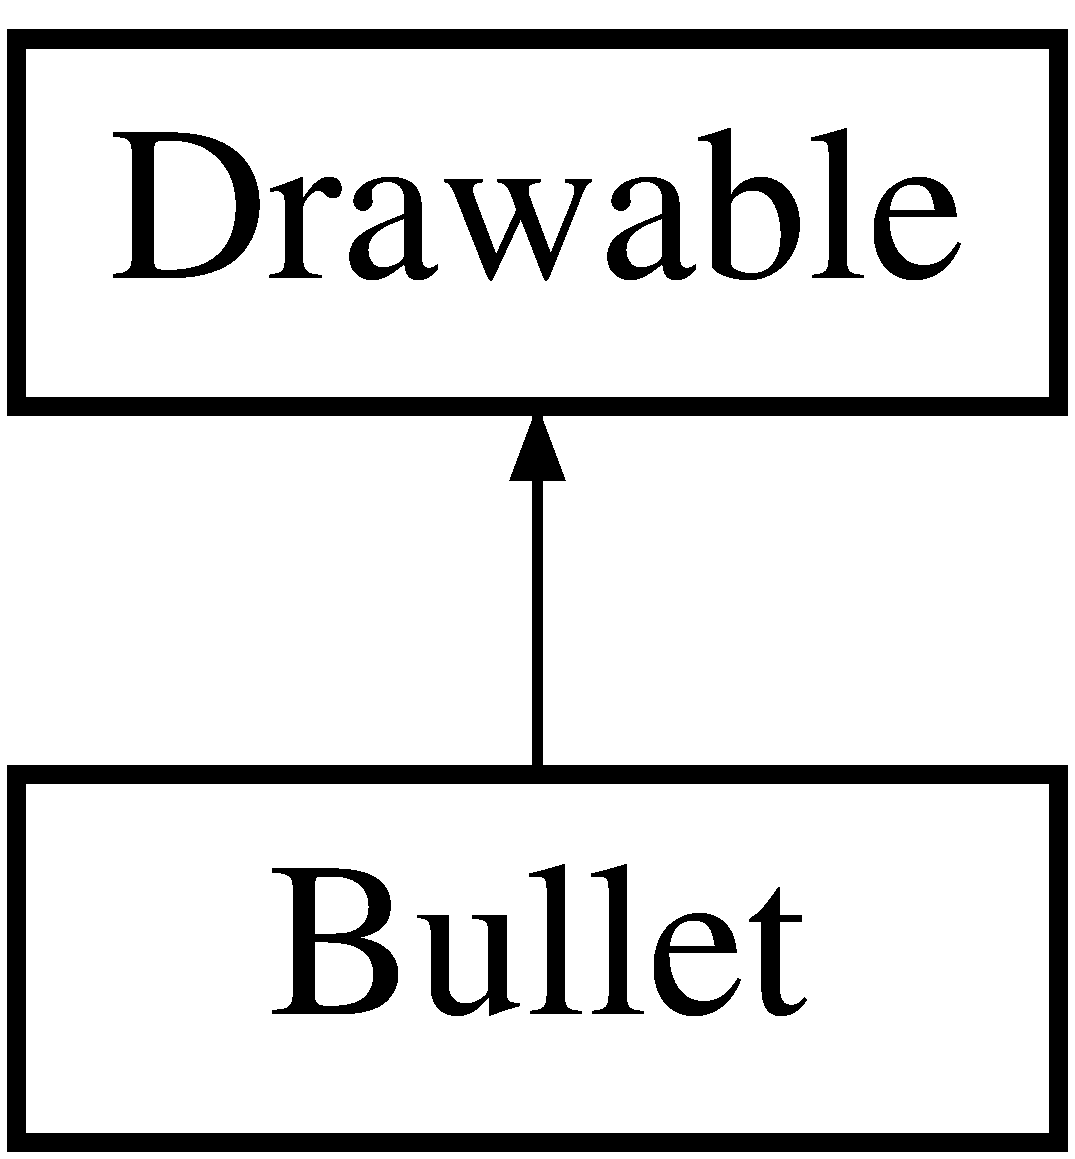
\includegraphics[height=2.000000cm]{class_bullet}
\end{center}
\end{figure}
\subsection*{Metody publiczne}
\begin{DoxyCompactItemize}
\item 
\mbox{\hyperlink{class_bullet_a5e8fd8844271779a2e6cf28a72b54da9}{Bullet}} ()=delete
\begin{DoxyCompactList}\small\item\em Konstruktor domyślny który jest usunięty. \end{DoxyCompactList}\item 
\mbox{\hyperlink{class_bullet_a9e0d7efa717b245dec0f436d5b3fe0c1}{Bullet}} (float x, float y)
\begin{DoxyCompactList}\small\item\em konstruktor pocisku \end{DoxyCompactList}\item 
virtual \mbox{\hyperlink{class_bullet_a051f364dc1951449fc0a3eb50537e681}{$\sim$\+Bullet}} ()=default
\begin{DoxyCompactList}\small\item\em Destruktor domyślny. \end{DoxyCompactList}\item 
void \mbox{\hyperlink{class_bullet_a34f6859e7b7e11fef77acbe8c58e84f8}{set\+Scale}} (float scale)
\begin{DoxyCompactList}\small\item\em Ustawia skale pocisku. \end{DoxyCompactList}\item 
void \mbox{\hyperlink{class_bullet_ad80b48a0ec4a81fad7e8fce823be2663}{set\+Rotation}} (float rotation)
\begin{DoxyCompactList}\small\item\em Ustawia rotacje pocisku. \end{DoxyCompactList}\item 
sf\+::\+Sprite \mbox{\hyperlink{class_bullet_a6808b8e55c477d41e24adc92d7726ad2}{get\+Sprite}} () const
\begin{DoxyCompactList}\small\item\em Zwraca obiekt wyświetlającego się pocisku. \end{DoxyCompactList}\item 
void \mbox{\hyperlink{class_bullet_a1a518fd30f6af391e54d6e4fe1382bf9}{set\+Velocity}} (sf\+::\+Vector2f velocity)
\begin{DoxyCompactList}\small\item\em Ustawia wektor prędkości pocisku. \end{DoxyCompactList}\item 
void \mbox{\hyperlink{class_bullet_a2bb01459022a349fb8e7bd82d0a53283}{set\+Velocity}} (float x, float y=0)
\begin{DoxyCompactList}\small\item\em Ustawia wektor prędkości pocisku. \end{DoxyCompactList}\item 
sf\+::\+Vector2f \mbox{\hyperlink{class_bullet_a1b48210b12476530fcc4da1baf6cf44c}{get\+Velocity}} () const
\begin{DoxyCompactList}\small\item\em Zwraca wektor prędkości pocisku. \end{DoxyCompactList}\item 
float \mbox{\hyperlink{class_bullet_ab9d387e9b8149d347a63bc82cede9549}{get\+PosX}} () const
\begin{DoxyCompactList}\small\item\em Zwraca X pozycji pocisku na ekranie. \end{DoxyCompactList}\item 
float \mbox{\hyperlink{class_bullet_a06183fe0cba63d671a05fc8e19102966}{get\+PosY}} () const
\begin{DoxyCompactList}\small\item\em Zwraca Y pozycji pocisku na ekranie. \end{DoxyCompactList}\item 
void \mbox{\hyperlink{class_bullet_a3e9ef53d97f7f26289b2a6a7a62b2184}{set\+PosX}} (float x)
\begin{DoxyCompactList}\small\item\em Ustawia wartość X pozycji pocisku na ekranie. \end{DoxyCompactList}\item 
void \mbox{\hyperlink{class_bullet_a600b82ffa52d709ac44db182a2b02c78}{set\+PosY}} (float y)
\begin{DoxyCompactList}\small\item\em Ustawia wartość Y pozycji pocisku na ekranie. \end{DoxyCompactList}\item 
void \mbox{\hyperlink{class_bullet_a32f4a0611fe2dd245fee955d14ca1f68}{update}} ()
\begin{DoxyCompactList}\small\item\em Aktualizuje obiekt co klatke. \end{DoxyCompactList}\item 
float \mbox{\hyperlink{class_bullet_a252b146bfd709799990523fcbb0c6a4b}{get\+Scale}} () const
\begin{DoxyCompactList}\small\item\em Zwraca wartość skali pocisku. \end{DoxyCompactList}\item 
void \mbox{\hyperlink{class_bullet_ae6b6d87e11805a0e76f04fb7187d674e}{set\+Scale\+Vector}} (sf\+::\+Vector2f scale)
\begin{DoxyCompactList}\small\item\em Ustawia wektor skali pocisku. \end{DoxyCompactList}\item 
sf\+::\+Vector2f \mbox{\hyperlink{class_bullet_a506586cdb96da5f682ea48139627096d}{get\+Scale\+Vector}} () const
\begin{DoxyCompactList}\small\item\em Zwraca wektor skali pocisku. \end{DoxyCompactList}\end{DoxyCompactItemize}
\subsection*{Metody chronione}
\begin{DoxyCompactItemize}
\item 
void \mbox{\hyperlink{class_bullet_a36d1d889cfc8095dcd9631a766b35cf0}{draw}} (sf\+::\+Render\+Target \&target, sf\+::\+Render\+States states) const override
\begin{DoxyCompactList}\small\item\em Rysuje obiekt na ekranie (dzidziczona z S\+F\+ML) \end{DoxyCompactList}\end{DoxyCompactItemize}


\subsection{Opis szczegółowy}
Klasa pocisku. 

Definicja w linii 10 pliku Bullet.\+h.



\subsection{Dokumentacja konstruktora i destruktora}
\mbox{\Hypertarget{class_bullet_a5e8fd8844271779a2e6cf28a72b54da9}\label{class_bullet_a5e8fd8844271779a2e6cf28a72b54da9}} 
\index{Bullet@{Bullet}!Bullet@{Bullet}}
\index{Bullet@{Bullet}!Bullet@{Bullet}}
\subsubsection{\texorpdfstring{Bullet()}{Bullet()}\hspace{0.1cm}{\footnotesize\ttfamily [1/2]}}
{\footnotesize\ttfamily Bullet\+::\+Bullet (\begin{DoxyParamCaption}{ }\end{DoxyParamCaption})\hspace{0.3cm}{\ttfamily [delete]}}



Konstruktor domyślny który jest usunięty. 

\mbox{\Hypertarget{class_bullet_a9e0d7efa717b245dec0f436d5b3fe0c1}\label{class_bullet_a9e0d7efa717b245dec0f436d5b3fe0c1}} 
\index{Bullet@{Bullet}!Bullet@{Bullet}}
\index{Bullet@{Bullet}!Bullet@{Bullet}}
\subsubsection{\texorpdfstring{Bullet()}{Bullet()}\hspace{0.1cm}{\footnotesize\ttfamily [2/2]}}
{\footnotesize\ttfamily Bullet\+::\+Bullet (\begin{DoxyParamCaption}\item[{float}]{x,  }\item[{float}]{y }\end{DoxyParamCaption})}



konstruktor pocisku 


\begin{DoxyParams}{Parametry}
{\em x} & -\/ współrzędna X pojawienia się pocisku na ekranie \\
\hline
{\em y} & -\/ współrzędna Y pojawienia się pocisku na ekranie \\
\hline
\end{DoxyParams}


Definicja w linii 5 pliku Bullet.\+cpp.

\mbox{\Hypertarget{class_bullet_a051f364dc1951449fc0a3eb50537e681}\label{class_bullet_a051f364dc1951449fc0a3eb50537e681}} 
\index{Bullet@{Bullet}!````~Bullet@{$\sim$\+Bullet}}
\index{````~Bullet@{$\sim$\+Bullet}!Bullet@{Bullet}}
\subsubsection{\texorpdfstring{$\sim$\+Bullet()}{~Bullet()}}
{\footnotesize\ttfamily virtual Bullet\+::$\sim$\+Bullet (\begin{DoxyParamCaption}{ }\end{DoxyParamCaption})\hspace{0.3cm}{\ttfamily [virtual]}, {\ttfamily [default]}}



Destruktor domyślny. 



\subsection{Dokumentacja funkcji składowych}
\mbox{\Hypertarget{class_bullet_a36d1d889cfc8095dcd9631a766b35cf0}\label{class_bullet_a36d1d889cfc8095dcd9631a766b35cf0}} 
\index{Bullet@{Bullet}!draw@{draw}}
\index{draw@{draw}!Bullet@{Bullet}}
\subsubsection{\texorpdfstring{draw()}{draw()}}
{\footnotesize\ttfamily void Bullet\+::draw (\begin{DoxyParamCaption}\item[{sf\+::\+Render\+Target \&}]{target,  }\item[{sf\+::\+Render\+States}]{states }\end{DoxyParamCaption}) const\hspace{0.3cm}{\ttfamily [override]}, {\ttfamily [protected]}}



Rysuje obiekt na ekranie (dzidziczona z S\+F\+ML) 


\begin{DoxyParams}{Parametry}
{\em target} & \\
\hline
{\em states} & \\
\hline
\end{DoxyParams}


Definicja w linii 94 pliku Bullet.\+cpp.

\mbox{\Hypertarget{class_bullet_ab9d387e9b8149d347a63bc82cede9549}\label{class_bullet_ab9d387e9b8149d347a63bc82cede9549}} 
\index{Bullet@{Bullet}!get\+PosX@{get\+PosX}}
\index{get\+PosX@{get\+PosX}!Bullet@{Bullet}}
\subsubsection{\texorpdfstring{get\+Pos\+X()}{getPosX()}}
{\footnotesize\ttfamily float Bullet\+::get\+PosX (\begin{DoxyParamCaption}{ }\end{DoxyParamCaption}) const}



Zwraca X pozycji pocisku na ekranie. 

\begin{DoxyReturn}{Zwraca}
X pozycji pocisku na ekranie 
\end{DoxyReturn}


Definicja w linii 49 pliku Bullet.\+cpp.

\mbox{\Hypertarget{class_bullet_a06183fe0cba63d671a05fc8e19102966}\label{class_bullet_a06183fe0cba63d671a05fc8e19102966}} 
\index{Bullet@{Bullet}!get\+PosY@{get\+PosY}}
\index{get\+PosY@{get\+PosY}!Bullet@{Bullet}}
\subsubsection{\texorpdfstring{get\+Pos\+Y()}{getPosY()}}
{\footnotesize\ttfamily float Bullet\+::get\+PosY (\begin{DoxyParamCaption}{ }\end{DoxyParamCaption}) const}



Zwraca Y pozycji pocisku na ekranie. 

\begin{DoxyReturn}{Zwraca}
Y pozycji pocisku na ekranie 
\end{DoxyReturn}


Definicja w linii 54 pliku Bullet.\+cpp.

\mbox{\Hypertarget{class_bullet_a252b146bfd709799990523fcbb0c6a4b}\label{class_bullet_a252b146bfd709799990523fcbb0c6a4b}} 
\index{Bullet@{Bullet}!get\+Scale@{get\+Scale}}
\index{get\+Scale@{get\+Scale}!Bullet@{Bullet}}
\subsubsection{\texorpdfstring{get\+Scale()}{getScale()}}
{\footnotesize\ttfamily float Bullet\+::get\+Scale (\begin{DoxyParamCaption}{ }\end{DoxyParamCaption}) const}



Zwraca wartość skali pocisku. 

\begin{DoxyReturn}{Zwraca}
wartość skali pocisku 
\end{DoxyReturn}


Definicja w linii 78 pliku Bullet.\+cpp.

\mbox{\Hypertarget{class_bullet_a506586cdb96da5f682ea48139627096d}\label{class_bullet_a506586cdb96da5f682ea48139627096d}} 
\index{Bullet@{Bullet}!get\+Scale\+Vector@{get\+Scale\+Vector}}
\index{get\+Scale\+Vector@{get\+Scale\+Vector}!Bullet@{Bullet}}
\subsubsection{\texorpdfstring{get\+Scale\+Vector()}{getScaleVector()}}
{\footnotesize\ttfamily sf\+::\+Vector2f Bullet\+::get\+Scale\+Vector (\begin{DoxyParamCaption}{ }\end{DoxyParamCaption}) const}



Zwraca wektor skali pocisku. 

\begin{DoxyReturn}{Zwraca}
wektor skali pocisku 
\end{DoxyReturn}


Definicja w linii 88 pliku Bullet.\+cpp.

\mbox{\Hypertarget{class_bullet_a6808b8e55c477d41e24adc92d7726ad2}\label{class_bullet_a6808b8e55c477d41e24adc92d7726ad2}} 
\index{Bullet@{Bullet}!get\+Sprite@{get\+Sprite}}
\index{get\+Sprite@{get\+Sprite}!Bullet@{Bullet}}
\subsubsection{\texorpdfstring{get\+Sprite()}{getSprite()}}
{\footnotesize\ttfamily sf\+::\+Sprite Bullet\+::get\+Sprite (\begin{DoxyParamCaption}{ }\end{DoxyParamCaption}) const}



Zwraca obiekt wyświetlającego się pocisku. 

\begin{DoxyReturn}{Zwraca}
obiekt sprite\textquotesingle{}a pocisku 
\end{DoxyReturn}


Definicja w linii 28 pliku Bullet.\+cpp.

\mbox{\Hypertarget{class_bullet_a1b48210b12476530fcc4da1baf6cf44c}\label{class_bullet_a1b48210b12476530fcc4da1baf6cf44c}} 
\index{Bullet@{Bullet}!get\+Velocity@{get\+Velocity}}
\index{get\+Velocity@{get\+Velocity}!Bullet@{Bullet}}
\subsubsection{\texorpdfstring{get\+Velocity()}{getVelocity()}}
{\footnotesize\ttfamily sf\+::\+Vector2f Bullet\+::get\+Velocity (\begin{DoxyParamCaption}{ }\end{DoxyParamCaption}) const}



Zwraca wektor prędkości pocisku. 

\begin{DoxyReturn}{Zwraca}
wektor prędkości pocisku 
\end{DoxyReturn}


Definicja w linii 44 pliku Bullet.\+cpp.

\mbox{\Hypertarget{class_bullet_a3e9ef53d97f7f26289b2a6a7a62b2184}\label{class_bullet_a3e9ef53d97f7f26289b2a6a7a62b2184}} 
\index{Bullet@{Bullet}!set\+PosX@{set\+PosX}}
\index{set\+PosX@{set\+PosX}!Bullet@{Bullet}}
\subsubsection{\texorpdfstring{set\+Pos\+X()}{setPosX()}}
{\footnotesize\ttfamily void Bullet\+::set\+PosX (\begin{DoxyParamCaption}\item[{float}]{x }\end{DoxyParamCaption})}



Ustawia wartość X pozycji pocisku na ekranie. 


\begin{DoxyParams}{Parametry}
{\em x} & -\/ współrzędna X pocisku na ekranie \\
\hline
\end{DoxyParams}


Definicja w linii 59 pliku Bullet.\+cpp.

\mbox{\Hypertarget{class_bullet_a600b82ffa52d709ac44db182a2b02c78}\label{class_bullet_a600b82ffa52d709ac44db182a2b02c78}} 
\index{Bullet@{Bullet}!set\+PosY@{set\+PosY}}
\index{set\+PosY@{set\+PosY}!Bullet@{Bullet}}
\subsubsection{\texorpdfstring{set\+Pos\+Y()}{setPosY()}}
{\footnotesize\ttfamily void Bullet\+::set\+PosY (\begin{DoxyParamCaption}\item[{float}]{y }\end{DoxyParamCaption})}



Ustawia wartość Y pozycji pocisku na ekranie. 


\begin{DoxyParams}{Parametry}
{\em y} & -\/ współrzędna Y pocisku na ekranie \\
\hline
\end{DoxyParams}


Definicja w linii 64 pliku Bullet.\+cpp.

\mbox{\Hypertarget{class_bullet_ad80b48a0ec4a81fad7e8fce823be2663}\label{class_bullet_ad80b48a0ec4a81fad7e8fce823be2663}} 
\index{Bullet@{Bullet}!set\+Rotation@{set\+Rotation}}
\index{set\+Rotation@{set\+Rotation}!Bullet@{Bullet}}
\subsubsection{\texorpdfstring{set\+Rotation()}{setRotation()}}
{\footnotesize\ttfamily void Bullet\+::set\+Rotation (\begin{DoxyParamCaption}\item[{float}]{rotation }\end{DoxyParamCaption})}



Ustawia rotacje pocisku. 


\begin{DoxyParams}{Parametry}
{\em rotation} & -\/ rotacja pocisku \\
\hline
\end{DoxyParams}


Definicja w linii 23 pliku Bullet.\+cpp.

\mbox{\Hypertarget{class_bullet_a34f6859e7b7e11fef77acbe8c58e84f8}\label{class_bullet_a34f6859e7b7e11fef77acbe8c58e84f8}} 
\index{Bullet@{Bullet}!set\+Scale@{set\+Scale}}
\index{set\+Scale@{set\+Scale}!Bullet@{Bullet}}
\subsubsection{\texorpdfstring{set\+Scale()}{setScale()}}
{\footnotesize\ttfamily void Bullet\+::set\+Scale (\begin{DoxyParamCaption}\item[{float}]{scale }\end{DoxyParamCaption})}



Ustawia skale pocisku. 


\begin{DoxyParams}{Parametry}
{\em scale} & -\/ skala pocisku \\
\hline
\end{DoxyParams}


Definicja w linii 18 pliku Bullet.\+cpp.

\mbox{\Hypertarget{class_bullet_ae6b6d87e11805a0e76f04fb7187d674e}\label{class_bullet_ae6b6d87e11805a0e76f04fb7187d674e}} 
\index{Bullet@{Bullet}!set\+Scale\+Vector@{set\+Scale\+Vector}}
\index{set\+Scale\+Vector@{set\+Scale\+Vector}!Bullet@{Bullet}}
\subsubsection{\texorpdfstring{set\+Scale\+Vector()}{setScaleVector()}}
{\footnotesize\ttfamily void Bullet\+::set\+Scale\+Vector (\begin{DoxyParamCaption}\item[{sf\+::\+Vector2f}]{scale }\end{DoxyParamCaption})}



Ustawia wektor skali pocisku. 


\begin{DoxyParams}{Parametry}
{\em scale} & -\/ wektor skali pocisku \\
\hline
\end{DoxyParams}


Definicja w linii 83 pliku Bullet.\+cpp.

\mbox{\Hypertarget{class_bullet_a1a518fd30f6af391e54d6e4fe1382bf9}\label{class_bullet_a1a518fd30f6af391e54d6e4fe1382bf9}} 
\index{Bullet@{Bullet}!set\+Velocity@{set\+Velocity}}
\index{set\+Velocity@{set\+Velocity}!Bullet@{Bullet}}
\subsubsection{\texorpdfstring{set\+Velocity()}{setVelocity()}\hspace{0.1cm}{\footnotesize\ttfamily [1/2]}}
{\footnotesize\ttfamily void Bullet\+::set\+Velocity (\begin{DoxyParamCaption}\item[{sf\+::\+Vector2f}]{velocity }\end{DoxyParamCaption})}



Ustawia wektor prędkości pocisku. 


\begin{DoxyParams}{Parametry}
{\em velocity} & -\/ wektor prędkości pocisku \\
\hline
\end{DoxyParams}


Definicja w linii 33 pliku Bullet.\+cpp.

\mbox{\Hypertarget{class_bullet_a2bb01459022a349fb8e7bd82d0a53283}\label{class_bullet_a2bb01459022a349fb8e7bd82d0a53283}} 
\index{Bullet@{Bullet}!set\+Velocity@{set\+Velocity}}
\index{set\+Velocity@{set\+Velocity}!Bullet@{Bullet}}
\subsubsection{\texorpdfstring{set\+Velocity()}{setVelocity()}\hspace{0.1cm}{\footnotesize\ttfamily [2/2]}}
{\footnotesize\ttfamily void Bullet\+::set\+Velocity (\begin{DoxyParamCaption}\item[{float}]{x,  }\item[{float}]{y = {\ttfamily 0} }\end{DoxyParamCaption})}



Ustawia wektor prędkości pocisku. 


\begin{DoxyParams}{Parametry}
{\em x} & -\/ składowa X wektora prędkości pocisku \\
\hline
{\em y} & -\/ składowa Y wektora prędkości pocisku \\
\hline
\end{DoxyParams}


Definicja w linii 38 pliku Bullet.\+cpp.

\mbox{\Hypertarget{class_bullet_a32f4a0611fe2dd245fee955d14ca1f68}\label{class_bullet_a32f4a0611fe2dd245fee955d14ca1f68}} 
\index{Bullet@{Bullet}!update@{update}}
\index{update@{update}!Bullet@{Bullet}}
\subsubsection{\texorpdfstring{update()}{update()}}
{\footnotesize\ttfamily void Bullet\+::update (\begin{DoxyParamCaption}{ }\end{DoxyParamCaption})}



Aktualizuje obiekt co klatke. 



Definicja w linii 69 pliku Bullet.\+cpp.



Dokumentacja dla tej klasy została wygenerowana z plików\+:\begin{DoxyCompactItemize}
\item 
D\+:/\+Projekty/\+C++/\+Programowanie w C2/\+Worms 2\+D/\+Worms 2\+D/\mbox{\hyperlink{_bullet_8h}{Bullet.\+h}}\item 
D\+:/\+Projekty/\+C++/\+Programowanie w C2/\+Worms 2\+D/\+Worms 2\+D/\mbox{\hyperlink{_bullet_8cpp}{Bullet.\+cpp}}\end{DoxyCompactItemize}

\hypertarget{class_button}{}\section{Dokumentacja klasy Button}
\label{class_button}\index{Button@{Button}}


{\ttfamily \#include $<$Button.\+h$>$}

Diagram dziedziczenia dla Button\begin{figure}[H]
\begin{center}
\leavevmode
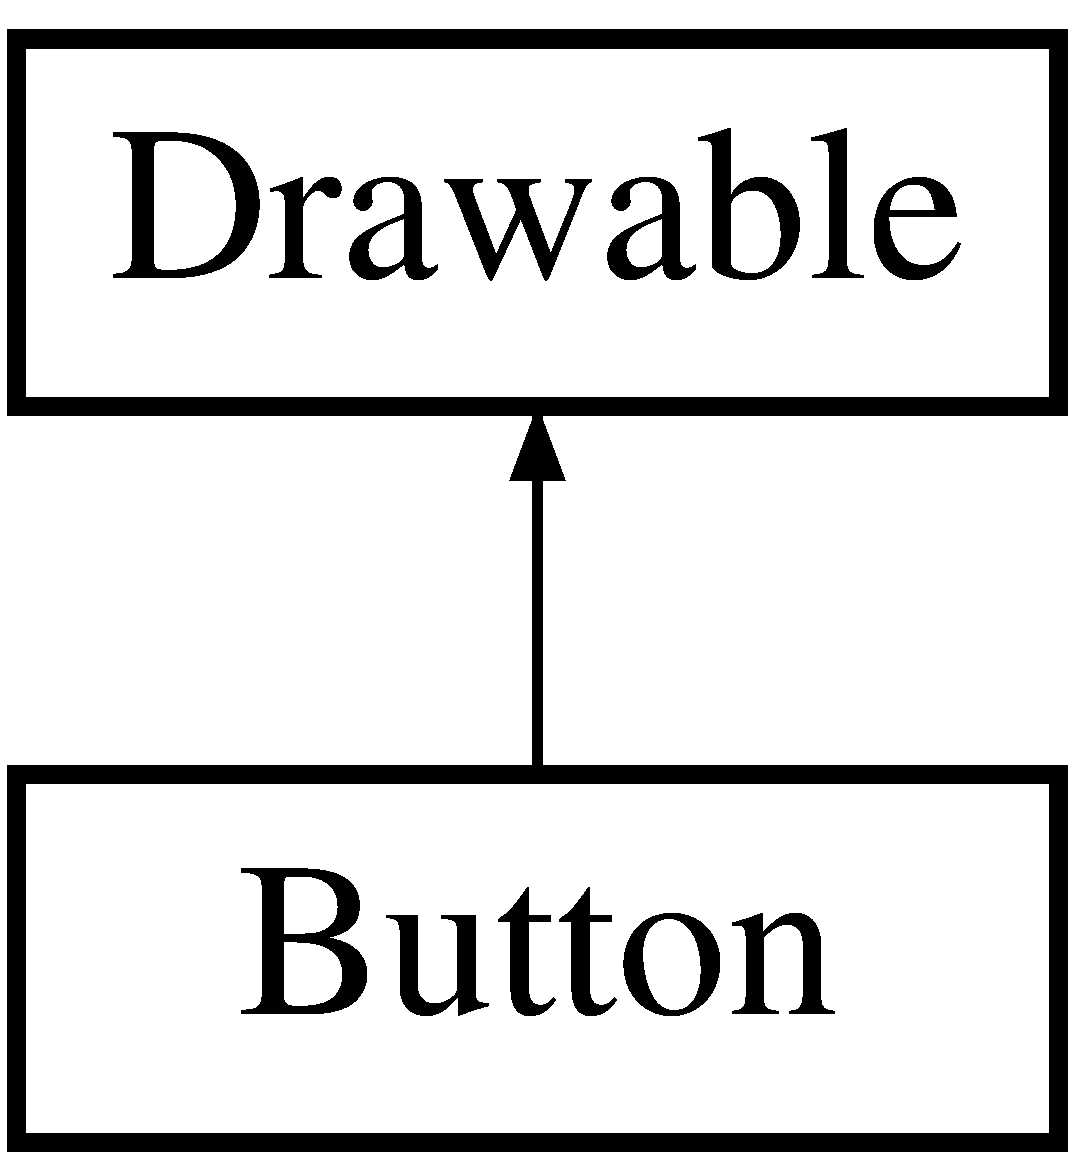
\includegraphics[height=2.000000cm]{class_button}
\end{center}
\end{figure}
\subsection*{Metody publiczne}
\begin{DoxyCompactItemize}
\item 
\mbox{\hyperlink{class_button_aeb4926acd6beafa022e3152b7ecbb992}{Button}} (float position\+\_\+x, float position\+\_\+y, const char $\ast$label, int id)
\begin{DoxyCompactList}\small\item\em konstruktor przycisku \end{DoxyCompactList}\item 
sf\+::\+Vector2f \mbox{\hyperlink{class_button_a0860c867e652f08390c05929d6837c13}{get\+Size}} ()
\begin{DoxyCompactList}\small\item\em Zwraca rozmiar buttona. \end{DoxyCompactList}\item 
sf\+::\+Vector2f \mbox{\hyperlink{class_button_aa5acd27eed9dc39a80051436b30ebd41}{get\+Position}} ()
\begin{DoxyCompactList}\small\item\em Zwraca wektor pozycji buttona. \end{DoxyCompactList}\item 
void \mbox{\hyperlink{class_button_a1a5ca19ed8efe0ea27625217dcab9f2c}{hover}} ()
\begin{DoxyCompactList}\small\item\em Podswietla przycisk. \end{DoxyCompactList}\item 
void \mbox{\hyperlink{class_button_a2fc33ec22217562b28ac6f02bda26c6e}{click}} ()
\begin{DoxyCompactList}\small\item\em Obs�uguje wci�ni�cie przycisku. \end{DoxyCompactList}\item 
void \mbox{\hyperlink{class_button_a31dfd83213a96fce828037745fc7e18f}{clear}} ()
\begin{DoxyCompactList}\small\item\em Czy�ci przycisk. \end{DoxyCompactList}\item 
bool \mbox{\hyperlink{class_button_a70c28ee3bec38814f77e6606e2da19ef}{is\+Hovered}} ()
\begin{DoxyCompactList}\small\item\em Sprawdza czy myszka jest na przycisku. \end{DoxyCompactList}\item 
bool \mbox{\hyperlink{class_button_acd766bf2e64e1aa93ad4c8a16b343347}{is\+Clicked}} ()
\begin{DoxyCompactList}\small\item\em Sprawdza czy przycisk zosta� kliniety. \end{DoxyCompactList}\item 
void \mbox{\hyperlink{class_button_a1a41668f07d7c7b03f05ab6602aa83e7}{set\+Color\+Default}} ()
\begin{DoxyCompactList}\small\item\em Ustawia kolor domy�lny przycisku. \end{DoxyCompactList}\item 
void \mbox{\hyperlink{class_button_a0f71bfa269ec47509592cb2e4bed9a90}{set\+Color\+Hovered}} ()
\begin{DoxyCompactList}\small\item\em Ustawia kolor pod�wietlenia przycisku. \end{DoxyCompactList}\item 
void \mbox{\hyperlink{class_button_acbc078483f6c6a6c75b7ff00cf07dd05}{set\+Color\+Clicked}} ()
\begin{DoxyCompactList}\small\item\em Ustawia kolor klikni�tego przycisku. \end{DoxyCompactList}\item 
int \mbox{\hyperlink{class_button_a0b024eb643308f2cfa8d13cd93c6b1ca}{get\+Id}} ()
\begin{DoxyCompactList}\small\item\em Zwraca ID przycisku. \end{DoxyCompactList}\end{DoxyCompactItemize}
\subsection*{Metody chronione}
\begin{DoxyCompactItemize}
\item 
void \mbox{\hyperlink{class_button_a94b2be0ad227968afccae8bc297ed99a}{draw}} (sf\+::\+Render\+Target \&target, sf\+::\+Render\+States states) const override
\begin{DoxyCompactList}\small\item\em Rysuje obiekt na ekranie (dzidziczona z S\+F\+ML) \end{DoxyCompactList}\end{DoxyCompactItemize}


\subsection{Opis szczegółowy}


Definicja w linii 3 pliku Button.\+h.



\subsection{Dokumentacja konstruktora i destruktora}
\mbox{\Hypertarget{class_button_aeb4926acd6beafa022e3152b7ecbb992}\label{class_button_aeb4926acd6beafa022e3152b7ecbb992}} 
\index{Button@{Button}!Button@{Button}}
\index{Button@{Button}!Button@{Button}}
\subsubsection{\texorpdfstring{Button()}{Button()}}
{\footnotesize\ttfamily Button\+::\+Button (\begin{DoxyParamCaption}\item[{float}]{position\+\_\+x,  }\item[{float}]{position\+\_\+y,  }\item[{const char $\ast$}]{label,  }\item[{int}]{id }\end{DoxyParamCaption})}



konstruktor przycisku 


\begin{DoxyParams}{Parametry}
{\em position\+\_\+x} & -\/ pozycja X przycisku na ekranie \\
\hline
{\em position\+\_\+y} & -\/ pozycja Y przycisku na ekranie \\
\hline
{\em label} & -\/ tekst na przycisku \\
\hline
{\em id} & -\/ id przycisku \\
\hline
\end{DoxyParams}


Definicja w linii 4 pliku Button.\+cpp.



\subsection{Dokumentacja funkcji składowych}
\mbox{\Hypertarget{class_button_a31dfd83213a96fce828037745fc7e18f}\label{class_button_a31dfd83213a96fce828037745fc7e18f}} 
\index{Button@{Button}!clear@{clear}}
\index{clear@{clear}!Button@{Button}}
\subsubsection{\texorpdfstring{clear()}{clear()}}
{\footnotesize\ttfamily void Button\+::clear (\begin{DoxyParamCaption}{ }\end{DoxyParamCaption})}



Czy�ci przycisk. 



Definicja w linii 60 pliku Button.\+cpp.

\mbox{\Hypertarget{class_button_a2fc33ec22217562b28ac6f02bda26c6e}\label{class_button_a2fc33ec22217562b28ac6f02bda26c6e}} 
\index{Button@{Button}!click@{click}}
\index{click@{click}!Button@{Button}}
\subsubsection{\texorpdfstring{click()}{click()}}
{\footnotesize\ttfamily void Button\+::click (\begin{DoxyParamCaption}{ }\end{DoxyParamCaption})}



Obs�uguje wci�ni�cie przycisku. 



Definicja w linii 54 pliku Button.\+cpp.

\mbox{\Hypertarget{class_button_a94b2be0ad227968afccae8bc297ed99a}\label{class_button_a94b2be0ad227968afccae8bc297ed99a}} 
\index{Button@{Button}!draw@{draw}}
\index{draw@{draw}!Button@{Button}}
\subsubsection{\texorpdfstring{draw()}{draw()}}
{\footnotesize\ttfamily void Button\+::draw (\begin{DoxyParamCaption}\item[{sf\+::\+Render\+Target \&}]{target,  }\item[{sf\+::\+Render\+States}]{states }\end{DoxyParamCaption}) const\hspace{0.3cm}{\ttfamily [override]}, {\ttfamily [protected]}}



Rysuje obiekt na ekranie (dzidziczona z S\+F\+ML) 


\begin{DoxyParams}{Parametry}
{\em target} & \\
\hline
{\em states} & \\
\hline
\end{DoxyParams}


Definicja w linii 31 pliku Button.\+cpp.

\mbox{\Hypertarget{class_button_a0b024eb643308f2cfa8d13cd93c6b1ca}\label{class_button_a0b024eb643308f2cfa8d13cd93c6b1ca}} 
\index{Button@{Button}!get\+Id@{get\+Id}}
\index{get\+Id@{get\+Id}!Button@{Button}}
\subsubsection{\texorpdfstring{get\+Id()}{getId()}}
{\footnotesize\ttfamily int Button\+::get\+Id (\begin{DoxyParamCaption}{ }\end{DoxyParamCaption})}



Zwraca ID przycisku. 

\begin{DoxyReturn}{Zwraca}
ID przycisku 
\end{DoxyReturn}


Definicja w linii 92 pliku Button.\+cpp.

\mbox{\Hypertarget{class_button_aa5acd27eed9dc39a80051436b30ebd41}\label{class_button_aa5acd27eed9dc39a80051436b30ebd41}} 
\index{Button@{Button}!get\+Position@{get\+Position}}
\index{get\+Position@{get\+Position}!Button@{Button}}
\subsubsection{\texorpdfstring{get\+Position()}{getPosition()}}
{\footnotesize\ttfamily sf\+::\+Vector2f Button\+::get\+Position (\begin{DoxyParamCaption}{ }\end{DoxyParamCaption})}



Zwraca wektor pozycji buttona. 

\begin{DoxyReturn}{Zwraca}
wektor pozycji buttona 
\end{DoxyReturn}


Definicja w linii 43 pliku Button.\+cpp.

\mbox{\Hypertarget{class_button_a0860c867e652f08390c05929d6837c13}\label{class_button_a0860c867e652f08390c05929d6837c13}} 
\index{Button@{Button}!get\+Size@{get\+Size}}
\index{get\+Size@{get\+Size}!Button@{Button}}
\subsubsection{\texorpdfstring{get\+Size()}{getSize()}}
{\footnotesize\ttfamily sf\+::\+Vector2f Button\+::get\+Size (\begin{DoxyParamCaption}{ }\end{DoxyParamCaption})}



Zwraca rozmiar buttona. 

\begin{DoxyReturn}{Zwraca}
wektor rozmiaru buttona 
\end{DoxyReturn}


Definicja w linii 38 pliku Button.\+cpp.

\mbox{\Hypertarget{class_button_a1a5ca19ed8efe0ea27625217dcab9f2c}\label{class_button_a1a5ca19ed8efe0ea27625217dcab9f2c}} 
\index{Button@{Button}!hover@{hover}}
\index{hover@{hover}!Button@{Button}}
\subsubsection{\texorpdfstring{hover()}{hover()}}
{\footnotesize\ttfamily void Button\+::hover (\begin{DoxyParamCaption}{ }\end{DoxyParamCaption})}



Podswietla przycisk. 



Definicja w linii 48 pliku Button.\+cpp.

\mbox{\Hypertarget{class_button_acd766bf2e64e1aa93ad4c8a16b343347}\label{class_button_acd766bf2e64e1aa93ad4c8a16b343347}} 
\index{Button@{Button}!is\+Clicked@{is\+Clicked}}
\index{is\+Clicked@{is\+Clicked}!Button@{Button}}
\subsubsection{\texorpdfstring{is\+Clicked()}{isClicked()}}
{\footnotesize\ttfamily bool Button\+::is\+Clicked (\begin{DoxyParamCaption}{ }\end{DoxyParamCaption})}



Sprawdza czy przycisk zosta� kliniety. 

\begin{DoxyReturn}{Zwraca}
czy przycisk zosta� kliniety 
\end{DoxyReturn}


Definicja w linii 72 pliku Button.\+cpp.

\mbox{\Hypertarget{class_button_a70c28ee3bec38814f77e6606e2da19ef}\label{class_button_a70c28ee3bec38814f77e6606e2da19ef}} 
\index{Button@{Button}!is\+Hovered@{is\+Hovered}}
\index{is\+Hovered@{is\+Hovered}!Button@{Button}}
\subsubsection{\texorpdfstring{is\+Hovered()}{isHovered()}}
{\footnotesize\ttfamily bool Button\+::is\+Hovered (\begin{DoxyParamCaption}{ }\end{DoxyParamCaption})}



Sprawdza czy myszka jest na przycisku. 

\begin{DoxyReturn}{Zwraca}
czy myszka jest na przycisku 
\end{DoxyReturn}


Definicja w linii 67 pliku Button.\+cpp.

\mbox{\Hypertarget{class_button_acbc078483f6c6a6c75b7ff00cf07dd05}\label{class_button_acbc078483f6c6a6c75b7ff00cf07dd05}} 
\index{Button@{Button}!set\+Color\+Clicked@{set\+Color\+Clicked}}
\index{set\+Color\+Clicked@{set\+Color\+Clicked}!Button@{Button}}
\subsubsection{\texorpdfstring{set\+Color\+Clicked()}{setColorClicked()}}
{\footnotesize\ttfamily void Button\+::set\+Color\+Clicked (\begin{DoxyParamCaption}{ }\end{DoxyParamCaption})}



Ustawia kolor klikni�tego przycisku. 



Definicja w linii 87 pliku Button.\+cpp.

\mbox{\Hypertarget{class_button_a1a41668f07d7c7b03f05ab6602aa83e7}\label{class_button_a1a41668f07d7c7b03f05ab6602aa83e7}} 
\index{Button@{Button}!set\+Color\+Default@{set\+Color\+Default}}
\index{set\+Color\+Default@{set\+Color\+Default}!Button@{Button}}
\subsubsection{\texorpdfstring{set\+Color\+Default()}{setColorDefault()}}
{\footnotesize\ttfamily void Button\+::set\+Color\+Default (\begin{DoxyParamCaption}{ }\end{DoxyParamCaption})}



Ustawia kolor domy�lny przycisku. 



Definicja w linii 77 pliku Button.\+cpp.

\mbox{\Hypertarget{class_button_a0f71bfa269ec47509592cb2e4bed9a90}\label{class_button_a0f71bfa269ec47509592cb2e4bed9a90}} 
\index{Button@{Button}!set\+Color\+Hovered@{set\+Color\+Hovered}}
\index{set\+Color\+Hovered@{set\+Color\+Hovered}!Button@{Button}}
\subsubsection{\texorpdfstring{set\+Color\+Hovered()}{setColorHovered()}}
{\footnotesize\ttfamily void Button\+::set\+Color\+Hovered (\begin{DoxyParamCaption}{ }\end{DoxyParamCaption})}



Ustawia kolor pod�wietlenia przycisku. 



Definicja w linii 82 pliku Button.\+cpp.



Dokumentacja dla tej klasy została wygenerowana z plików\+:\begin{DoxyCompactItemize}
\item 
D\+:/\+Projekty/\+C++/\+Programowanie w C2/\+Worms 2\+D/\+Worms 2\+D/\mbox{\hyperlink{_button_8h}{Button.\+h}}\item 
D\+:/\+Projekty/\+C++/\+Programowanie w C2/\+Worms 2\+D/\+Worms 2\+D/\mbox{\hyperlink{_button_8cpp}{Button.\+cpp}}\end{DoxyCompactItemize}

\hypertarget{class_f_p_s_counter}{}\section{Dokumentacja klasy F\+P\+S\+Counter}
\label{class_f_p_s_counter}\index{F\+P\+S\+Counter@{F\+P\+S\+Counter}}


{\ttfamily \#include $<$F\+P\+S\+Counter.\+h$>$}

\subsection*{Metody publiczne}
\begin{DoxyCompactItemize}
\item 
\mbox{\hyperlink{class_f_p_s_counter_ae565c465bd222c4f733813b402d232a8}{F\+P\+S\+Counter}} (unsigned int font\+Size=12)
\item 
void \mbox{\hyperlink{class_f_p_s_counter_abba94df2064bfa561ef9d1a3e11929a5}{start}} ()
\begin{DoxyCompactList}\small\item\em Uruchamia licznik. \end{DoxyCompactList}\item 
void \mbox{\hyperlink{class_f_p_s_counter_a7415ae4bb4094b4809627caf5e40d8f1}{draw\+F\+PS}} ()
\begin{DoxyCompactList}\small\item\em Rysuje ilość F\+PS na ekranie. \end{DoxyCompactList}\item 
void \mbox{\hyperlink{class_f_p_s_counter_a57be5e95f140cb230f3f4e11ca476857}{set\+Color}} (sf\+::\+Color color)
\begin{DoxyCompactList}\small\item\em Ustawia kolor licznika. \end{DoxyCompactList}\end{DoxyCompactItemize}


\subsection{Opis szczegółowy}


Definicja w linii 3 pliku F\+P\+S\+Counter.\+h.



\subsection{Dokumentacja konstruktora i destruktora}
\mbox{\Hypertarget{class_f_p_s_counter_ae565c465bd222c4f733813b402d232a8}\label{class_f_p_s_counter_ae565c465bd222c4f733813b402d232a8}} 
\index{F\+P\+S\+Counter@{F\+P\+S\+Counter}!F\+P\+S\+Counter@{F\+P\+S\+Counter}}
\index{F\+P\+S\+Counter@{F\+P\+S\+Counter}!F\+P\+S\+Counter@{F\+P\+S\+Counter}}
\subsubsection{\texorpdfstring{F\+P\+S\+Counter()}{FPSCounter()}}
{\footnotesize\ttfamily F\+P\+S\+Counter\+::\+F\+P\+S\+Counter (\begin{DoxyParamCaption}\item[{unsigned int}]{font\+Size = {\ttfamily 12} }\end{DoxyParamCaption})}

Konstruktor licznika F\+PS\textquotesingle{}ów (dla D\+E\+B\+B\+U\+GE\textquotesingle{}a)


\begin{DoxyParams}{Parametry}
{\em font\+Size} & -\/ rozmiar czcionki \\
\hline
\end{DoxyParams}


Definicja w linii 6 pliku F\+P\+S\+Counter.\+cpp.



\subsection{Dokumentacja funkcji składowych}
\mbox{\Hypertarget{class_f_p_s_counter_a7415ae4bb4094b4809627caf5e40d8f1}\label{class_f_p_s_counter_a7415ae4bb4094b4809627caf5e40d8f1}} 
\index{F\+P\+S\+Counter@{F\+P\+S\+Counter}!draw\+F\+PS@{draw\+F\+PS}}
\index{draw\+F\+PS@{draw\+F\+PS}!F\+P\+S\+Counter@{F\+P\+S\+Counter}}
\subsubsection{\texorpdfstring{draw\+F\+P\+S()}{drawFPS()}}
{\footnotesize\ttfamily void F\+P\+S\+Counter\+::draw\+F\+PS (\begin{DoxyParamCaption}{ }\end{DoxyParamCaption})}



Rysuje ilość F\+PS na ekranie. 



Definicja w linii 34 pliku F\+P\+S\+Counter.\+cpp.

\mbox{\Hypertarget{class_f_p_s_counter_a57be5e95f140cb230f3f4e11ca476857}\label{class_f_p_s_counter_a57be5e95f140cb230f3f4e11ca476857}} 
\index{F\+P\+S\+Counter@{F\+P\+S\+Counter}!set\+Color@{set\+Color}}
\index{set\+Color@{set\+Color}!F\+P\+S\+Counter@{F\+P\+S\+Counter}}
\subsubsection{\texorpdfstring{set\+Color()}{setColor()}}
{\footnotesize\ttfamily void F\+P\+S\+Counter\+::set\+Color (\begin{DoxyParamCaption}\item[{sf\+::\+Color}]{color }\end{DoxyParamCaption})}



Ustawia kolor licznika. 


\begin{DoxyParams}{Parametry}
{\em color} & -\/ kolor licznika \\
\hline
\end{DoxyParams}


Definicja w linii 42 pliku F\+P\+S\+Counter.\+cpp.

\mbox{\Hypertarget{class_f_p_s_counter_abba94df2064bfa561ef9d1a3e11929a5}\label{class_f_p_s_counter_abba94df2064bfa561ef9d1a3e11929a5}} 
\index{F\+P\+S\+Counter@{F\+P\+S\+Counter}!start@{start}}
\index{start@{start}!F\+P\+S\+Counter@{F\+P\+S\+Counter}}
\subsubsection{\texorpdfstring{start()}{start()}}
{\footnotesize\ttfamily void F\+P\+S\+Counter\+::start (\begin{DoxyParamCaption}{ }\end{DoxyParamCaption})}



Uruchamia licznik. 



Definicja w linii 20 pliku F\+P\+S\+Counter.\+cpp.



Dokumentacja dla tej klasy została wygenerowana z plików\+:\begin{DoxyCompactItemize}
\item 
D\+:/\+Projekty/\+C++/\+Programowanie w C2/\+Worms 2\+D/\+Worms 2\+D/\mbox{\hyperlink{_f_p_s_counter_8h}{F\+P\+S\+Counter.\+h}}\item 
D\+:/\+Projekty/\+C++/\+Programowanie w C2/\+Worms 2\+D/\+Worms 2\+D/\mbox{\hyperlink{_f_p_s_counter_8cpp}{F\+P\+S\+Counter.\+cpp}}\end{DoxyCompactItemize}

\hypertarget{class_game_event}{}\section{Dokumentacja klasy Game\+Event}
\label{class_game_event}\index{Game\+Event@{Game\+Event}}


{\ttfamily \#include $<$Game\+Event.\+h$>$}

\subsection*{Metody publiczne}
\begin{DoxyCompactItemize}
\item 
\mbox{\hyperlink{class_game_event_a0a8133b65ffc98712879d18186ef3020}{Game\+Event}} ()
\begin{DoxyCompactList}\small\item\em Konstruktor zdarzeń \end{DoxyCompactList}\item 
virtual \mbox{\hyperlink{class_game_event_aaf514ed35c80bbbcc54ce411d9d71eef}{$\sim$\+Game\+Event}} ()
\begin{DoxyCompactList}\small\item\em Destruktor zdarzeń \end{DoxyCompactList}\item 
sf\+::\+Event \mbox{\hyperlink{class_game_event_adbf21138a4eb40624a0f40b2ff75f6db}{Get\+Instance}} ()
\begin{DoxyCompactList}\small\item\em Zwraca instancje zdarzeń S\+F\+ML\textquotesingle{}a. \end{DoxyCompactList}\item 
void \mbox{\hyperlink{class_game_event_a73a56d31069079123f03f20855cb9bf0}{handle\+Events}} ()
\begin{DoxyCompactList}\small\item\em Obsługuje zdarzenia co klatke. \end{DoxyCompactList}\end{DoxyCompactItemize}
\subsection*{Statyczne metody publiczne}
\begin{DoxyCompactItemize}
\item 
static \mbox{\hyperlink{class_game_event}{Game\+Event}} $\ast$ \mbox{\hyperlink{class_game_event_a683bf5025fe1a31263cb96059fc9e5a5}{Get\+Event\+Instance}} ()
\begin{DoxyCompactList}\small\item\em Zwraca statyczny wskaźnik na obiekt Zdarzeń gry (Singleton) \end{DoxyCompactList}\end{DoxyCompactItemize}


\subsection{Opis szczegółowy}


Definicja w linii 5 pliku Game\+Event.\+h.



\subsection{Dokumentacja konstruktora i destruktora}
\mbox{\Hypertarget{class_game_event_a0a8133b65ffc98712879d18186ef3020}\label{class_game_event_a0a8133b65ffc98712879d18186ef3020}} 
\index{Game\+Event@{Game\+Event}!Game\+Event@{Game\+Event}}
\index{Game\+Event@{Game\+Event}!Game\+Event@{Game\+Event}}
\subsubsection{\texorpdfstring{Game\+Event()}{GameEvent()}}
{\footnotesize\ttfamily Game\+Event\+::\+Game\+Event (\begin{DoxyParamCaption}{ }\end{DoxyParamCaption})}



Konstruktor zdarzeń 



Definicja w linii 6 pliku Game\+Event.\+cpp.

\mbox{\Hypertarget{class_game_event_aaf514ed35c80bbbcc54ce411d9d71eef}\label{class_game_event_aaf514ed35c80bbbcc54ce411d9d71eef}} 
\index{Game\+Event@{Game\+Event}!````~Game\+Event@{$\sim$\+Game\+Event}}
\index{````~Game\+Event@{$\sim$\+Game\+Event}!Game\+Event@{Game\+Event}}
\subsubsection{\texorpdfstring{$\sim$\+Game\+Event()}{~GameEvent()}}
{\footnotesize\ttfamily Game\+Event\+::$\sim$\+Game\+Event (\begin{DoxyParamCaption}{ }\end{DoxyParamCaption})\hspace{0.3cm}{\ttfamily [virtual]}}



Destruktor zdarzeń 



Definicja w linii 19 pliku Game\+Event.\+cpp.



\subsection{Dokumentacja funkcji składowych}
\mbox{\Hypertarget{class_game_event_a683bf5025fe1a31263cb96059fc9e5a5}\label{class_game_event_a683bf5025fe1a31263cb96059fc9e5a5}} 
\index{Game\+Event@{Game\+Event}!Get\+Event\+Instance@{Get\+Event\+Instance}}
\index{Get\+Event\+Instance@{Get\+Event\+Instance}!Game\+Event@{Game\+Event}}
\subsubsection{\texorpdfstring{Get\+Event\+Instance()}{GetEventInstance()}}
{\footnotesize\ttfamily \mbox{\hyperlink{class_game_event}{Game\+Event}} $\ast$ Game\+Event\+::\+Get\+Event\+Instance (\begin{DoxyParamCaption}{ }\end{DoxyParamCaption})\hspace{0.3cm}{\ttfamily [static]}}



Zwraca statyczny wskaźnik na obiekt Zdarzeń gry (Singleton) 

\begin{DoxyReturn}{Zwraca}
wskaźnik na obiekt Zdarzeń gry 
\end{DoxyReturn}


Definicja w linii 383 pliku Game\+Event.\+cpp.

\mbox{\Hypertarget{class_game_event_adbf21138a4eb40624a0f40b2ff75f6db}\label{class_game_event_adbf21138a4eb40624a0f40b2ff75f6db}} 
\index{Game\+Event@{Game\+Event}!Get\+Instance@{Get\+Instance}}
\index{Get\+Instance@{Get\+Instance}!Game\+Event@{Game\+Event}}
\subsubsection{\texorpdfstring{Get\+Instance()}{GetInstance()}}
{\footnotesize\ttfamily sf\+::\+Event Game\+Event\+::\+Get\+Instance (\begin{DoxyParamCaption}{ }\end{DoxyParamCaption})}



Zwraca instancje zdarzeń S\+F\+ML\textquotesingle{}a. 

\begin{DoxyReturn}{Zwraca}
instancje zdarzeń S\+F\+ML\textquotesingle{}a 
\end{DoxyReturn}


Definicja w linii 23 pliku Game\+Event.\+cpp.

\mbox{\Hypertarget{class_game_event_a73a56d31069079123f03f20855cb9bf0}\label{class_game_event_a73a56d31069079123f03f20855cb9bf0}} 
\index{Game\+Event@{Game\+Event}!handle\+Events@{handle\+Events}}
\index{handle\+Events@{handle\+Events}!Game\+Event@{Game\+Event}}
\subsubsection{\texorpdfstring{handle\+Events()}{handleEvents()}}
{\footnotesize\ttfamily void Game\+Event\+::handle\+Events (\begin{DoxyParamCaption}{ }\end{DoxyParamCaption})}



Obsługuje zdarzenia co klatke. 



Definicja w linii 28 pliku Game\+Event.\+cpp.



Dokumentacja dla tej klasy została wygenerowana z plików\+:\begin{DoxyCompactItemize}
\item 
D\+:/\+Projekty/\+C++/\+Programowanie w C2/\+Worms 2\+D/\+Worms 2\+D/\mbox{\hyperlink{_game_event_8h}{Game\+Event.\+h}}\item 
D\+:/\+Projekty/\+C++/\+Programowanie w C2/\+Worms 2\+D/\+Worms 2\+D/\mbox{\hyperlink{_game_event_8cpp}{Game\+Event.\+cpp}}\end{DoxyCompactItemize}

\hypertarget{class_game_sound}{}\section{Dokumentacja klasy Game\+Sound}
\label{class_game_sound}\index{Game\+Sound@{Game\+Sound}}


{\ttfamily \#include $<$Game\+Sound.\+h$>$}

\subsection*{Metody publiczne}
\begin{DoxyCompactItemize}
\item 
\mbox{\hyperlink{class_game_sound_a14feacd320c8a89e68cacf456920c8c1}{Game\+Sound}} ()
\begin{DoxyCompactList}\small\item\em Konstruktor. \end{DoxyCompactList}\item 
void \mbox{\hyperlink{class_game_sound_ad89f0cfad75194e895cb68437f9c231f}{Play\+Main\+Music}} ()
\begin{DoxyCompactList}\small\item\em Odtwarza główne audio w grze. \end{DoxyCompactList}\item 
void \mbox{\hyperlink{class_game_sound_a30db244babc1e4aa518bd56500cea028}{Start\+Sample}} ()
\begin{DoxyCompactList}\small\item\em Odtwarza odgłos worma. \end{DoxyCompactList}\item 
void \mbox{\hyperlink{class_game_sound_a9b64e35e47dd7f06876be460c9cbf67f}{Pause\+Sample}} ()
\begin{DoxyCompactList}\small\item\em Pauzuje odgłos worma. \end{DoxyCompactList}\item 
void \mbox{\hyperlink{class_game_sound_a819246ab2ca8154f7b8fa1b87cdd68ca}{Stop\+Sample}} ()
\begin{DoxyCompactList}\small\item\em Stopuje odgłos worma. \end{DoxyCompactList}\item 
void \mbox{\hyperlink{class_game_sound_a909e0c0bc44437ea2853e734ab548e5a}{Start\+Revolver\+Sound}} ()
\begin{DoxyCompactList}\small\item\em Odtwarza odgłos wystrzału rewolwera. \end{DoxyCompactList}\item 
void \mbox{\hyperlink{class_game_sound_a88651691b6b8e28f14e73778805bd898}{Stop\+Revolver\+Sound}} ()
\begin{DoxyCompactList}\small\item\em Stopuje odtwarzanie odgłosu wystrzału rewolwera. \end{DoxyCompactList}\item 
void \mbox{\hyperlink{class_game_sound_ab3bc96f5be15c7a9be79a035ec16638c}{Start\+Bazooka\+Sound}} ()
\begin{DoxyCompactList}\small\item\em Odtwarza odgłos wystrzału bazooki. \end{DoxyCompactList}\item 
void \mbox{\hyperlink{class_game_sound_a90742af83bd0006dba5e9a5129214c9a}{Stop\+Bazooka\+Sound}} ()
\begin{DoxyCompactList}\small\item\em Stopuje odtwarzanie odgłosu wystrzału bazooki. \end{DoxyCompactList}\item 
void \mbox{\hyperlink{class_game_sound_acd0ef105f4731da50afe47b3e02558a2}{Play\+Death}} ()
\begin{DoxyCompactList}\small\item\em Odtwarza dźwięk śmierci worma. \end{DoxyCompactList}\item 
void \mbox{\hyperlink{class_game_sound_accb7034b9c796bc9270fc3a724d18821}{Stop\+Death}} ()
\begin{DoxyCompactList}\small\item\em Stopuje dźwięk śmierci worma. \end{DoxyCompactList}\item 
void \mbox{\hyperlink{class_game_sound_a429befa039bfc4e9f7b33326fbb090a4}{Play\+Win}} ()
\begin{DoxyCompactList}\small\item\em Odtwarza dźwięk zwycięstwa. \end{DoxyCompactList}\item 
void \mbox{\hyperlink{class_game_sound_a1001607a8791e3000aff36fcc2d949f3}{Stop\+Win}} ()
\begin{DoxyCompactList}\small\item\em Stopuje dźwięk zwycięstwa. \end{DoxyCompactList}\end{DoxyCompactItemize}


\subsection{Opis szczegółowy}


Definicja w linii 5 pliku Game\+Sound.\+h.



\subsection{Dokumentacja konstruktora i destruktora}
\mbox{\Hypertarget{class_game_sound_a14feacd320c8a89e68cacf456920c8c1}\label{class_game_sound_a14feacd320c8a89e68cacf456920c8c1}} 
\index{Game\+Sound@{Game\+Sound}!Game\+Sound@{Game\+Sound}}
\index{Game\+Sound@{Game\+Sound}!Game\+Sound@{Game\+Sound}}
\subsubsection{\texorpdfstring{Game\+Sound()}{GameSound()}}
{\footnotesize\ttfamily Game\+Sound\+::\+Game\+Sound (\begin{DoxyParamCaption}{ }\end{DoxyParamCaption})}



Konstruktor. 



Definicja w linii 3 pliku Game\+Sound.\+cpp.



\subsection{Dokumentacja funkcji składowych}
\mbox{\Hypertarget{class_game_sound_a9b64e35e47dd7f06876be460c9cbf67f}\label{class_game_sound_a9b64e35e47dd7f06876be460c9cbf67f}} 
\index{Game\+Sound@{Game\+Sound}!Pause\+Sample@{Pause\+Sample}}
\index{Pause\+Sample@{Pause\+Sample}!Game\+Sound@{Game\+Sound}}
\subsubsection{\texorpdfstring{Pause\+Sample()}{PauseSample()}}
{\footnotesize\ttfamily void Game\+Sound\+::\+Pause\+Sample (\begin{DoxyParamCaption}{ }\end{DoxyParamCaption})}



Pauzuje odgłos worma. 



Definicja w linii 47 pliku Game\+Sound.\+cpp.

\mbox{\Hypertarget{class_game_sound_acd0ef105f4731da50afe47b3e02558a2}\label{class_game_sound_acd0ef105f4731da50afe47b3e02558a2}} 
\index{Game\+Sound@{Game\+Sound}!Play\+Death@{Play\+Death}}
\index{Play\+Death@{Play\+Death}!Game\+Sound@{Game\+Sound}}
\subsubsection{\texorpdfstring{Play\+Death()}{PlayDeath()}}
{\footnotesize\ttfamily void Game\+Sound\+::\+Play\+Death (\begin{DoxyParamCaption}{ }\end{DoxyParamCaption})}



Odtwarza dźwięk śmierci worma. 



Definicja w linii 77 pliku Game\+Sound.\+cpp.

\mbox{\Hypertarget{class_game_sound_ad89f0cfad75194e895cb68437f9c231f}\label{class_game_sound_ad89f0cfad75194e895cb68437f9c231f}} 
\index{Game\+Sound@{Game\+Sound}!Play\+Main\+Music@{Play\+Main\+Music}}
\index{Play\+Main\+Music@{Play\+Main\+Music}!Game\+Sound@{Game\+Sound}}
\subsubsection{\texorpdfstring{Play\+Main\+Music()}{PlayMainMusic()}}
{\footnotesize\ttfamily void Game\+Sound\+::\+Play\+Main\+Music (\begin{DoxyParamCaption}{ }\end{DoxyParamCaption})}



Odtwarza główne audio w grze. 



Definicja w linii 37 pliku Game\+Sound.\+cpp.

\mbox{\Hypertarget{class_game_sound_a429befa039bfc4e9f7b33326fbb090a4}\label{class_game_sound_a429befa039bfc4e9f7b33326fbb090a4}} 
\index{Game\+Sound@{Game\+Sound}!Play\+Win@{Play\+Win}}
\index{Play\+Win@{Play\+Win}!Game\+Sound@{Game\+Sound}}
\subsubsection{\texorpdfstring{Play\+Win()}{PlayWin()}}
{\footnotesize\ttfamily void Game\+Sound\+::\+Play\+Win (\begin{DoxyParamCaption}{ }\end{DoxyParamCaption})}



Odtwarza dźwięk zwycięstwa. 



Definicja w linii 87 pliku Game\+Sound.\+cpp.

\mbox{\Hypertarget{class_game_sound_ab3bc96f5be15c7a9be79a035ec16638c}\label{class_game_sound_ab3bc96f5be15c7a9be79a035ec16638c}} 
\index{Game\+Sound@{Game\+Sound}!Start\+Bazooka\+Sound@{Start\+Bazooka\+Sound}}
\index{Start\+Bazooka\+Sound@{Start\+Bazooka\+Sound}!Game\+Sound@{Game\+Sound}}
\subsubsection{\texorpdfstring{Start\+Bazooka\+Sound()}{StartBazookaSound()}}
{\footnotesize\ttfamily void Game\+Sound\+::\+Start\+Bazooka\+Sound (\begin{DoxyParamCaption}{ }\end{DoxyParamCaption})}



Odtwarza odgłos wystrzału bazooki. 



Definicja w linii 67 pliku Game\+Sound.\+cpp.

\mbox{\Hypertarget{class_game_sound_a909e0c0bc44437ea2853e734ab548e5a}\label{class_game_sound_a909e0c0bc44437ea2853e734ab548e5a}} 
\index{Game\+Sound@{Game\+Sound}!Start\+Revolver\+Sound@{Start\+Revolver\+Sound}}
\index{Start\+Revolver\+Sound@{Start\+Revolver\+Sound}!Game\+Sound@{Game\+Sound}}
\subsubsection{\texorpdfstring{Start\+Revolver\+Sound()}{StartRevolverSound()}}
{\footnotesize\ttfamily void Game\+Sound\+::\+Start\+Revolver\+Sound (\begin{DoxyParamCaption}{ }\end{DoxyParamCaption})}



Odtwarza odgłos wystrzału rewolwera. 



Definicja w linii 57 pliku Game\+Sound.\+cpp.

\mbox{\Hypertarget{class_game_sound_a30db244babc1e4aa518bd56500cea028}\label{class_game_sound_a30db244babc1e4aa518bd56500cea028}} 
\index{Game\+Sound@{Game\+Sound}!Start\+Sample@{Start\+Sample}}
\index{Start\+Sample@{Start\+Sample}!Game\+Sound@{Game\+Sound}}
\subsubsection{\texorpdfstring{Start\+Sample()}{StartSample()}}
{\footnotesize\ttfamily void Game\+Sound\+::\+Start\+Sample (\begin{DoxyParamCaption}{ }\end{DoxyParamCaption})}



Odtwarza odgłos worma. 



Definicja w linii 42 pliku Game\+Sound.\+cpp.

\mbox{\Hypertarget{class_game_sound_a90742af83bd0006dba5e9a5129214c9a}\label{class_game_sound_a90742af83bd0006dba5e9a5129214c9a}} 
\index{Game\+Sound@{Game\+Sound}!Stop\+Bazooka\+Sound@{Stop\+Bazooka\+Sound}}
\index{Stop\+Bazooka\+Sound@{Stop\+Bazooka\+Sound}!Game\+Sound@{Game\+Sound}}
\subsubsection{\texorpdfstring{Stop\+Bazooka\+Sound()}{StopBazookaSound()}}
{\footnotesize\ttfamily void Game\+Sound\+::\+Stop\+Bazooka\+Sound (\begin{DoxyParamCaption}{ }\end{DoxyParamCaption})}



Stopuje odtwarzanie odgłosu wystrzału bazooki. 



Definicja w linii 72 pliku Game\+Sound.\+cpp.

\mbox{\Hypertarget{class_game_sound_accb7034b9c796bc9270fc3a724d18821}\label{class_game_sound_accb7034b9c796bc9270fc3a724d18821}} 
\index{Game\+Sound@{Game\+Sound}!Stop\+Death@{Stop\+Death}}
\index{Stop\+Death@{Stop\+Death}!Game\+Sound@{Game\+Sound}}
\subsubsection{\texorpdfstring{Stop\+Death()}{StopDeath()}}
{\footnotesize\ttfamily void Game\+Sound\+::\+Stop\+Death (\begin{DoxyParamCaption}{ }\end{DoxyParamCaption})}



Stopuje dźwięk śmierci worma. 



Definicja w linii 82 pliku Game\+Sound.\+cpp.

\mbox{\Hypertarget{class_game_sound_a88651691b6b8e28f14e73778805bd898}\label{class_game_sound_a88651691b6b8e28f14e73778805bd898}} 
\index{Game\+Sound@{Game\+Sound}!Stop\+Revolver\+Sound@{Stop\+Revolver\+Sound}}
\index{Stop\+Revolver\+Sound@{Stop\+Revolver\+Sound}!Game\+Sound@{Game\+Sound}}
\subsubsection{\texorpdfstring{Stop\+Revolver\+Sound()}{StopRevolverSound()}}
{\footnotesize\ttfamily void Game\+Sound\+::\+Stop\+Revolver\+Sound (\begin{DoxyParamCaption}{ }\end{DoxyParamCaption})}



Stopuje odtwarzanie odgłosu wystrzału rewolwera. 



Definicja w linii 62 pliku Game\+Sound.\+cpp.

\mbox{\Hypertarget{class_game_sound_a819246ab2ca8154f7b8fa1b87cdd68ca}\label{class_game_sound_a819246ab2ca8154f7b8fa1b87cdd68ca}} 
\index{Game\+Sound@{Game\+Sound}!Stop\+Sample@{Stop\+Sample}}
\index{Stop\+Sample@{Stop\+Sample}!Game\+Sound@{Game\+Sound}}
\subsubsection{\texorpdfstring{Stop\+Sample()}{StopSample()}}
{\footnotesize\ttfamily void Game\+Sound\+::\+Stop\+Sample (\begin{DoxyParamCaption}{ }\end{DoxyParamCaption})}



Stopuje odgłos worma. 



Definicja w linii 52 pliku Game\+Sound.\+cpp.

\mbox{\Hypertarget{class_game_sound_a1001607a8791e3000aff36fcc2d949f3}\label{class_game_sound_a1001607a8791e3000aff36fcc2d949f3}} 
\index{Game\+Sound@{Game\+Sound}!Stop\+Win@{Stop\+Win}}
\index{Stop\+Win@{Stop\+Win}!Game\+Sound@{Game\+Sound}}
\subsubsection{\texorpdfstring{Stop\+Win()}{StopWin()}}
{\footnotesize\ttfamily void Game\+Sound\+::\+Stop\+Win (\begin{DoxyParamCaption}{ }\end{DoxyParamCaption})}



Stopuje dźwięk zwycięstwa. 



Definicja w linii 92 pliku Game\+Sound.\+cpp.



Dokumentacja dla tej klasy została wygenerowana z plików\+:\begin{DoxyCompactItemize}
\item 
D\+:/\+Projekty/\+C++/\+Programowanie w C2/\+Worms 2\+D/\+Worms 2\+D/\mbox{\hyperlink{_game_sound_8h}{Game\+Sound.\+h}}\item 
D\+:/\+Projekty/\+C++/\+Programowanie w C2/\+Worms 2\+D/\+Worms 2\+D/\mbox{\hyperlink{_game_sound_8cpp}{Game\+Sound.\+cpp}}\end{DoxyCompactItemize}

\hypertarget{class_game_window}{}\section{Dokumentacja klasy Game\+Window}
\label{class_game_window}\index{Game\+Window@{Game\+Window}}


{\ttfamily \#include $<$Game\+Window.\+h$>$}

\subsection*{Metody publiczne}
\begin{DoxyCompactItemize}
\item 
\mbox{\hyperlink{class_game_window_aeb8fe4d63cdd9e9d3e6fdcb35d15a37c}{Game\+Window}} ()=delete
\item 
\mbox{\hyperlink{class_game_window_a55b071c0390e45c064a160c1e6baaa08}{$\sim$\+Game\+Window}} ()
\item 
\mbox{\hyperlink{class_game_window_a22da49d930c2fd26888b223049a9da18}{Game\+Window}} (unsigned int width, unsigned int height, std\+::string name)
\item 
sf\+::\+Render\+Window $\ast$ \mbox{\hyperlink{class_game_window_aa5ef8ededf54c333a5b19344b95220de}{Get\+Instance}} () const
\item 
void \mbox{\hyperlink{class_game_window_af2b8df98b008a25d8c64f67cd6f23f59}{Change\+Frame\+Limit}} (unsigned int limit=60) const
\item 
void \mbox{\hyperlink{class_game_window_a7dcdd3731da278a522c59a72ecee77b3}{Main\+Loop}} ()
\item 
void \mbox{\hyperlink{class_game_window_a043804fa483c8ea2f348b6fb1dac4e4a}{Update\+Worms}} (int i)
\item 
void \mbox{\hyperlink{class_game_window_aa6659ccbd2a5d27141eb3f00fdc72ea6}{Update\+WormsB}} (int i)
\item 
\mbox{\hyperlink{class_worm}{Worm}} $\ast$$\ast$ \mbox{\hyperlink{class_game_window_a172c7184152f5c49a5089205ae3528f5}{Get\+Current\+Worm}} ()
\item 
std\+::vector$<$ \mbox{\hyperlink{class_worm}{Worm}} $\ast$ $>$ $\ast$ \mbox{\hyperlink{class_game_window_a7535403f5d3ab3ffe22c711665102052}{Get\+Worms\+Array}} () const
\item 
std\+::vector$<$ \mbox{\hyperlink{class_worm}{Worm}} $\ast$ $>$ $\ast$ \mbox{\hyperlink{class_game_window_ab9695e10e5a991a9df920911402b9272}{Get\+Worms\+ArrayB}} () const
\item 
int \mbox{\hyperlink{class_game_window_acfef11596afd262e0e4e77051ed24cde}{Get\+Worm\+Count}} () const
\item 
int \mbox{\hyperlink{class_game_window_a6c6d7e7da6cfc12d33c6da6f84596b15}{Get\+Worm\+CountB}} () const
\item 
int $\ast$ \mbox{\hyperlink{class_game_window_a67485df550fda5b1cc0aa6e7644f72e8}{Get\+Current\+Team}} ()
\item 
int $\ast$ \mbox{\hyperlink{class_game_window_a6dbc377a22fff8ab01f30b10337dc5ae}{Get\+Current\+Worm\+ID}} ()
\item 
void \mbox{\hyperlink{class_game_window_a856649fd2f3954b6ae3c6cf9da6b17a6}{Set\+Background\+Color}} (sf\+::\+Color color)
\item 
\mbox{\hyperlink{class_game_sound}{Game\+Sound}} $\ast$ \mbox{\hyperlink{class_game_window_aa3280056f0018da1eee85ccb1e5fd2ac}{Get\+Game\+Sound}} () const
\item 
void \mbox{\hyperlink{class_game_window_a735db6bd1918401c3b36502d14c8fd7b}{Switch\+To\+Red\+Team}} ()
\item 
void \mbox{\hyperlink{class_game_window_aa7c5976b188b842fc2ce45190b55bdfa}{Switch\+To\+Blue\+Team}} ()
\item 
void \mbox{\hyperlink{class_game_window_a24b9dd0b93ad629da3b2e15661fdea0c}{Set\+Choose\+States}} ()
\end{DoxyCompactItemize}
\subsection*{Statyczne metody publiczne}
\begin{DoxyCompactItemize}
\item 
static \mbox{\hyperlink{class_game_window}{Game\+Window}} $\ast$ \mbox{\hyperlink{class_game_window_a9c480a3795bfd6d22a9dc8a3bae47b1b}{Get\+Game\+Window\+Instance}} (unsigned int width=1280, unsigned int height=1024, std\+::string name=\char`\"{}Worms 2\+D\char`\"{})
\end{DoxyCompactItemize}
\subsection*{Atrybuty publiczne}
\begin{DoxyCompactItemize}
\item 
\mbox{\hyperlink{class_terrain}{Terrain}} \mbox{\hyperlink{class_game_window_ab5d02e9738d1f7f3fea4cd146172cf11}{terrain}}
\item 
\mbox{\hyperlink{class_menu}{Menu}} \mbox{\hyperlink{class_game_window_a3c63dc36f53ecb9b1d055923293daffd}{menu}}
\item 
int \mbox{\hyperlink{class_game_window_aafe2b1768f704b81e4fe94115287b9f7}{game\+\_\+state}}
\item 
bool \mbox{\hyperlink{class_game_window_a5ce0d59c491a490bc1d98afcac741016}{game\+\_\+started}}
\end{DoxyCompactItemize}


\subsection{Opis szczegółowy}


Definicja w linii 14 pliku Game\+Window.\+h.



\subsection{Dokumentacja konstruktora i destruktora}
\mbox{\Hypertarget{class_game_window_aeb8fe4d63cdd9e9d3e6fdcb35d15a37c}\label{class_game_window_aeb8fe4d63cdd9e9d3e6fdcb35d15a37c}} 
\index{Game\+Window@{Game\+Window}!Game\+Window@{Game\+Window}}
\index{Game\+Window@{Game\+Window}!Game\+Window@{Game\+Window}}
\subsubsection{\texorpdfstring{Game\+Window()}{GameWindow()}\hspace{0.1cm}{\footnotesize\ttfamily [1/2]}}
{\footnotesize\ttfamily Game\+Window\+::\+Game\+Window (\begin{DoxyParamCaption}{ }\end{DoxyParamCaption})\hspace{0.3cm}{\ttfamily [delete]}}

\mbox{\Hypertarget{class_game_window_a55b071c0390e45c064a160c1e6baaa08}\label{class_game_window_a55b071c0390e45c064a160c1e6baaa08}} 
\index{Game\+Window@{Game\+Window}!````~Game\+Window@{$\sim$\+Game\+Window}}
\index{````~Game\+Window@{$\sim$\+Game\+Window}!Game\+Window@{Game\+Window}}
\subsubsection{\texorpdfstring{$\sim$\+Game\+Window()}{~GameWindow()}}
{\footnotesize\ttfamily Game\+Window\+::$\sim$\+Game\+Window (\begin{DoxyParamCaption}{ }\end{DoxyParamCaption})}



Definicja w linii 26 pliku Game\+Window.\+cpp.

\mbox{\Hypertarget{class_game_window_a22da49d930c2fd26888b223049a9da18}\label{class_game_window_a22da49d930c2fd26888b223049a9da18}} 
\index{Game\+Window@{Game\+Window}!Game\+Window@{Game\+Window}}
\index{Game\+Window@{Game\+Window}!Game\+Window@{Game\+Window}}
\subsubsection{\texorpdfstring{Game\+Window()}{GameWindow()}\hspace{0.1cm}{\footnotesize\ttfamily [2/2]}}
{\footnotesize\ttfamily Game\+Window\+::\+Game\+Window (\begin{DoxyParamCaption}\item[{unsigned int}]{width,  }\item[{unsigned int}]{height,  }\item[{std\+::string}]{name }\end{DoxyParamCaption})}



Definicja w linii 4 pliku Game\+Window.\+cpp.



\subsection{Dokumentacja funkcji składowych}
\mbox{\Hypertarget{class_game_window_af2b8df98b008a25d8c64f67cd6f23f59}\label{class_game_window_af2b8df98b008a25d8c64f67cd6f23f59}} 
\index{Game\+Window@{Game\+Window}!Change\+Frame\+Limit@{Change\+Frame\+Limit}}
\index{Change\+Frame\+Limit@{Change\+Frame\+Limit}!Game\+Window@{Game\+Window}}
\subsubsection{\texorpdfstring{Change\+Frame\+Limit()}{ChangeFrameLimit()}}
{\footnotesize\ttfamily void Game\+Window\+::\+Change\+Frame\+Limit (\begin{DoxyParamCaption}\item[{unsigned int}]{limit = {\ttfamily 60} }\end{DoxyParamCaption}) const}



Definicja w linii 37 pliku Game\+Window.\+cpp.

\mbox{\Hypertarget{class_game_window_a67485df550fda5b1cc0aa6e7644f72e8}\label{class_game_window_a67485df550fda5b1cc0aa6e7644f72e8}} 
\index{Game\+Window@{Game\+Window}!Get\+Current\+Team@{Get\+Current\+Team}}
\index{Get\+Current\+Team@{Get\+Current\+Team}!Game\+Window@{Game\+Window}}
\subsubsection{\texorpdfstring{Get\+Current\+Team()}{GetCurrentTeam()}}
{\footnotesize\ttfamily int $\ast$ Game\+Window\+::\+Get\+Current\+Team (\begin{DoxyParamCaption}{ }\end{DoxyParamCaption})}



Definicja w linii 293 pliku Game\+Window.\+cpp.

\mbox{\Hypertarget{class_game_window_a172c7184152f5c49a5089205ae3528f5}\label{class_game_window_a172c7184152f5c49a5089205ae3528f5}} 
\index{Game\+Window@{Game\+Window}!Get\+Current\+Worm@{Get\+Current\+Worm}}
\index{Get\+Current\+Worm@{Get\+Current\+Worm}!Game\+Window@{Game\+Window}}
\subsubsection{\texorpdfstring{Get\+Current\+Worm()}{GetCurrentWorm()}}
{\footnotesize\ttfamily \mbox{\hyperlink{class_worm}{Worm}} $\ast$$\ast$ Game\+Window\+::\+Get\+Current\+Worm (\begin{DoxyParamCaption}{ }\end{DoxyParamCaption})}



Definicja w linii 268 pliku Game\+Window.\+cpp.

\mbox{\Hypertarget{class_game_window_a6dbc377a22fff8ab01f30b10337dc5ae}\label{class_game_window_a6dbc377a22fff8ab01f30b10337dc5ae}} 
\index{Game\+Window@{Game\+Window}!Get\+Current\+Worm\+ID@{Get\+Current\+Worm\+ID}}
\index{Get\+Current\+Worm\+ID@{Get\+Current\+Worm\+ID}!Game\+Window@{Game\+Window}}
\subsubsection{\texorpdfstring{Get\+Current\+Worm\+I\+D()}{GetCurrentWormID()}}
{\footnotesize\ttfamily int $\ast$ Game\+Window\+::\+Get\+Current\+Worm\+ID (\begin{DoxyParamCaption}{ }\end{DoxyParamCaption})}



Definicja w linii 298 pliku Game\+Window.\+cpp.

\mbox{\Hypertarget{class_game_window_aa3280056f0018da1eee85ccb1e5fd2ac}\label{class_game_window_aa3280056f0018da1eee85ccb1e5fd2ac}} 
\index{Game\+Window@{Game\+Window}!Get\+Game\+Sound@{Get\+Game\+Sound}}
\index{Get\+Game\+Sound@{Get\+Game\+Sound}!Game\+Window@{Game\+Window}}
\subsubsection{\texorpdfstring{Get\+Game\+Sound()}{GetGameSound()}}
{\footnotesize\ttfamily \mbox{\hyperlink{class_game_sound}{Game\+Sound}} $\ast$ Game\+Window\+::\+Get\+Game\+Sound (\begin{DoxyParamCaption}{ }\end{DoxyParamCaption}) const}



Definicja w linii 308 pliku Game\+Window.\+cpp.

\mbox{\Hypertarget{class_game_window_a9c480a3795bfd6d22a9dc8a3bae47b1b}\label{class_game_window_a9c480a3795bfd6d22a9dc8a3bae47b1b}} 
\index{Game\+Window@{Game\+Window}!Get\+Game\+Window\+Instance@{Get\+Game\+Window\+Instance}}
\index{Get\+Game\+Window\+Instance@{Get\+Game\+Window\+Instance}!Game\+Window@{Game\+Window}}
\subsubsection{\texorpdfstring{Get\+Game\+Window\+Instance()}{GetGameWindowInstance()}}
{\footnotesize\ttfamily \mbox{\hyperlink{class_game_window}{Game\+Window}} $\ast$ Game\+Window\+::\+Get\+Game\+Window\+Instance (\begin{DoxyParamCaption}\item[{unsigned int}]{width = {\ttfamily 1280},  }\item[{unsigned int}]{height = {\ttfamily 1024},  }\item[{std\+::string}]{name = {\ttfamily \char`\"{}Worms~2D\char`\"{}} }\end{DoxyParamCaption})\hspace{0.3cm}{\ttfamily [static]}}



Definicja w linii 373 pliku Game\+Window.\+cpp.

\mbox{\Hypertarget{class_game_window_aa5ef8ededf54c333a5b19344b95220de}\label{class_game_window_aa5ef8ededf54c333a5b19344b95220de}} 
\index{Game\+Window@{Game\+Window}!Get\+Instance@{Get\+Instance}}
\index{Get\+Instance@{Get\+Instance}!Game\+Window@{Game\+Window}}
\subsubsection{\texorpdfstring{Get\+Instance()}{GetInstance()}}
{\footnotesize\ttfamily sf\+::\+Render\+Window $\ast$ Game\+Window\+::\+Get\+Instance (\begin{DoxyParamCaption}{ }\end{DoxyParamCaption}) const}



Definicja w linii 32 pliku Game\+Window.\+cpp.

\mbox{\Hypertarget{class_game_window_acfef11596afd262e0e4e77051ed24cde}\label{class_game_window_acfef11596afd262e0e4e77051ed24cde}} 
\index{Game\+Window@{Game\+Window}!Get\+Worm\+Count@{Get\+Worm\+Count}}
\index{Get\+Worm\+Count@{Get\+Worm\+Count}!Game\+Window@{Game\+Window}}
\subsubsection{\texorpdfstring{Get\+Worm\+Count()}{GetWormCount()}}
{\footnotesize\ttfamily int Game\+Window\+::\+Get\+Worm\+Count (\begin{DoxyParamCaption}{ }\end{DoxyParamCaption}) const}



Definicja w linii 283 pliku Game\+Window.\+cpp.

\mbox{\Hypertarget{class_game_window_a6c6d7e7da6cfc12d33c6da6f84596b15}\label{class_game_window_a6c6d7e7da6cfc12d33c6da6f84596b15}} 
\index{Game\+Window@{Game\+Window}!Get\+Worm\+CountB@{Get\+Worm\+CountB}}
\index{Get\+Worm\+CountB@{Get\+Worm\+CountB}!Game\+Window@{Game\+Window}}
\subsubsection{\texorpdfstring{Get\+Worm\+Count\+B()}{GetWormCountB()}}
{\footnotesize\ttfamily int Game\+Window\+::\+Get\+Worm\+CountB (\begin{DoxyParamCaption}{ }\end{DoxyParamCaption}) const}



Definicja w linii 288 pliku Game\+Window.\+cpp.

\mbox{\Hypertarget{class_game_window_a7535403f5d3ab3ffe22c711665102052}\label{class_game_window_a7535403f5d3ab3ffe22c711665102052}} 
\index{Game\+Window@{Game\+Window}!Get\+Worms\+Array@{Get\+Worms\+Array}}
\index{Get\+Worms\+Array@{Get\+Worms\+Array}!Game\+Window@{Game\+Window}}
\subsubsection{\texorpdfstring{Get\+Worms\+Array()}{GetWormsArray()}}
{\footnotesize\ttfamily std\+::vector$<$ \mbox{\hyperlink{class_worm}{Worm}} $\ast$ $>$ $\ast$ Game\+Window\+::\+Get\+Worms\+Array (\begin{DoxyParamCaption}{ }\end{DoxyParamCaption}) const}



Definicja w linii 273 pliku Game\+Window.\+cpp.

\mbox{\Hypertarget{class_game_window_ab9695e10e5a991a9df920911402b9272}\label{class_game_window_ab9695e10e5a991a9df920911402b9272}} 
\index{Game\+Window@{Game\+Window}!Get\+Worms\+ArrayB@{Get\+Worms\+ArrayB}}
\index{Get\+Worms\+ArrayB@{Get\+Worms\+ArrayB}!Game\+Window@{Game\+Window}}
\subsubsection{\texorpdfstring{Get\+Worms\+Array\+B()}{GetWormsArrayB()}}
{\footnotesize\ttfamily std\+::vector$<$ \mbox{\hyperlink{class_worm}{Worm}} $\ast$ $>$ $\ast$ Game\+Window\+::\+Get\+Worms\+ArrayB (\begin{DoxyParamCaption}{ }\end{DoxyParamCaption}) const}



Definicja w linii 278 pliku Game\+Window.\+cpp.

\mbox{\Hypertarget{class_game_window_a7dcdd3731da278a522c59a72ecee77b3}\label{class_game_window_a7dcdd3731da278a522c59a72ecee77b3}} 
\index{Game\+Window@{Game\+Window}!Main\+Loop@{Main\+Loop}}
\index{Main\+Loop@{Main\+Loop}!Game\+Window@{Game\+Window}}
\subsubsection{\texorpdfstring{Main\+Loop()}{MainLoop()}}
{\footnotesize\ttfamily void Game\+Window\+::\+Main\+Loop (\begin{DoxyParamCaption}{ }\end{DoxyParamCaption})}



Definicja w linii 79 pliku Game\+Window.\+cpp.

\mbox{\Hypertarget{class_game_window_a856649fd2f3954b6ae3c6cf9da6b17a6}\label{class_game_window_a856649fd2f3954b6ae3c6cf9da6b17a6}} 
\index{Game\+Window@{Game\+Window}!Set\+Background\+Color@{Set\+Background\+Color}}
\index{Set\+Background\+Color@{Set\+Background\+Color}!Game\+Window@{Game\+Window}}
\subsubsection{\texorpdfstring{Set\+Background\+Color()}{SetBackgroundColor()}}
{\footnotesize\ttfamily void Game\+Window\+::\+Set\+Background\+Color (\begin{DoxyParamCaption}\item[{sf\+::\+Color}]{color }\end{DoxyParamCaption})}



Definicja w linii 303 pliku Game\+Window.\+cpp.

\mbox{\Hypertarget{class_game_window_a24b9dd0b93ad629da3b2e15661fdea0c}\label{class_game_window_a24b9dd0b93ad629da3b2e15661fdea0c}} 
\index{Game\+Window@{Game\+Window}!Set\+Choose\+States@{Set\+Choose\+States}}
\index{Set\+Choose\+States@{Set\+Choose\+States}!Game\+Window@{Game\+Window}}
\subsubsection{\texorpdfstring{Set\+Choose\+States()}{SetChooseStates()}}
{\footnotesize\ttfamily void Game\+Window\+::\+Set\+Choose\+States (\begin{DoxyParamCaption}{ }\end{DoxyParamCaption})}



Definicja w linii 340 pliku Game\+Window.\+cpp.

\mbox{\Hypertarget{class_game_window_aa7c5976b188b842fc2ce45190b55bdfa}\label{class_game_window_aa7c5976b188b842fc2ce45190b55bdfa}} 
\index{Game\+Window@{Game\+Window}!Switch\+To\+Blue\+Team@{Switch\+To\+Blue\+Team}}
\index{Switch\+To\+Blue\+Team@{Switch\+To\+Blue\+Team}!Game\+Window@{Game\+Window}}
\subsubsection{\texorpdfstring{Switch\+To\+Blue\+Team()}{SwitchToBlueTeam()}}
{\footnotesize\ttfamily void Game\+Window\+::\+Switch\+To\+Blue\+Team (\begin{DoxyParamCaption}{ }\end{DoxyParamCaption})}



Definicja w linii 332 pliku Game\+Window.\+cpp.

\mbox{\Hypertarget{class_game_window_a735db6bd1918401c3b36502d14c8fd7b}\label{class_game_window_a735db6bd1918401c3b36502d14c8fd7b}} 
\index{Game\+Window@{Game\+Window}!Switch\+To\+Red\+Team@{Switch\+To\+Red\+Team}}
\index{Switch\+To\+Red\+Team@{Switch\+To\+Red\+Team}!Game\+Window@{Game\+Window}}
\subsubsection{\texorpdfstring{Switch\+To\+Red\+Team()}{SwitchToRedTeam()}}
{\footnotesize\ttfamily void Game\+Window\+::\+Switch\+To\+Red\+Team (\begin{DoxyParamCaption}{ }\end{DoxyParamCaption})}



Definicja w linii 324 pliku Game\+Window.\+cpp.

\mbox{\Hypertarget{class_game_window_a043804fa483c8ea2f348b6fb1dac4e4a}\label{class_game_window_a043804fa483c8ea2f348b6fb1dac4e4a}} 
\index{Game\+Window@{Game\+Window}!Update\+Worms@{Update\+Worms}}
\index{Update\+Worms@{Update\+Worms}!Game\+Window@{Game\+Window}}
\subsubsection{\texorpdfstring{Update\+Worms()}{UpdateWorms()}}
{\footnotesize\ttfamily void Game\+Window\+::\+Update\+Worms (\begin{DoxyParamCaption}\item[{int}]{i }\end{DoxyParamCaption})}



Definicja w linii 258 pliku Game\+Window.\+cpp.

\mbox{\Hypertarget{class_game_window_aa6659ccbd2a5d27141eb3f00fdc72ea6}\label{class_game_window_aa6659ccbd2a5d27141eb3f00fdc72ea6}} 
\index{Game\+Window@{Game\+Window}!Update\+WormsB@{Update\+WormsB}}
\index{Update\+WormsB@{Update\+WormsB}!Game\+Window@{Game\+Window}}
\subsubsection{\texorpdfstring{Update\+Worms\+B()}{UpdateWormsB()}}
{\footnotesize\ttfamily void Game\+Window\+::\+Update\+WormsB (\begin{DoxyParamCaption}\item[{int}]{i }\end{DoxyParamCaption})}



Definicja w linii 263 pliku Game\+Window.\+cpp.



\subsection{Dokumentacja atrybutów składowych}
\mbox{\Hypertarget{class_game_window_a5ce0d59c491a490bc1d98afcac741016}\label{class_game_window_a5ce0d59c491a490bc1d98afcac741016}} 
\index{Game\+Window@{Game\+Window}!game\+\_\+started@{game\+\_\+started}}
\index{game\+\_\+started@{game\+\_\+started}!Game\+Window@{Game\+Window}}
\subsubsection{\texorpdfstring{game\+\_\+started}{game\_started}}
{\footnotesize\ttfamily bool Game\+Window\+::game\+\_\+started}



Definicja w linii 38 pliku Game\+Window.\+h.

\mbox{\Hypertarget{class_game_window_aafe2b1768f704b81e4fe94115287b9f7}\label{class_game_window_aafe2b1768f704b81e4fe94115287b9f7}} 
\index{Game\+Window@{Game\+Window}!game\+\_\+state@{game\+\_\+state}}
\index{game\+\_\+state@{game\+\_\+state}!Game\+Window@{Game\+Window}}
\subsubsection{\texorpdfstring{game\+\_\+state}{game\_state}}
{\footnotesize\ttfamily int Game\+Window\+::game\+\_\+state}



Definicja w linii 37 pliku Game\+Window.\+h.

\mbox{\Hypertarget{class_game_window_a3c63dc36f53ecb9b1d055923293daffd}\label{class_game_window_a3c63dc36f53ecb9b1d055923293daffd}} 
\index{Game\+Window@{Game\+Window}!menu@{menu}}
\index{menu@{menu}!Game\+Window@{Game\+Window}}
\subsubsection{\texorpdfstring{menu}{menu}}
{\footnotesize\ttfamily \mbox{\hyperlink{class_menu}{Menu}} Game\+Window\+::menu}



Definicja w linii 36 pliku Game\+Window.\+h.

\mbox{\Hypertarget{class_game_window_ab5d02e9738d1f7f3fea4cd146172cf11}\label{class_game_window_ab5d02e9738d1f7f3fea4cd146172cf11}} 
\index{Game\+Window@{Game\+Window}!terrain@{terrain}}
\index{terrain@{terrain}!Game\+Window@{Game\+Window}}
\subsubsection{\texorpdfstring{terrain}{terrain}}
{\footnotesize\ttfamily \mbox{\hyperlink{class_terrain}{Terrain}} Game\+Window\+::terrain}



Definicja w linii 35 pliku Game\+Window.\+h.



Dokumentacja dla tej klasy została wygenerowana z plików\+:\begin{DoxyCompactItemize}
\item 
D\+:/\+Projekty/\+C++/\+Programowanie w C2/\+Worms 2\+D/\+Worms 2\+D/\mbox{\hyperlink{_game_window_8h}{Game\+Window.\+h}}\item 
D\+:/\+Projekty/\+C++/\+Programowanie w C2/\+Worms 2\+D/\+Worms 2\+D/\mbox{\hyperlink{_game_window_8cpp}{Game\+Window.\+cpp}}\end{DoxyCompactItemize}

\hypertarget{class_menu}{}\section{Dokumentacja klasy Menu}
\label{class_menu}\index{Menu@{Menu}}


{\ttfamily \#include $<$Menu.\+h$>$}

Diagram dziedziczenia dla Menu\begin{figure}[H]
\begin{center}
\leavevmode
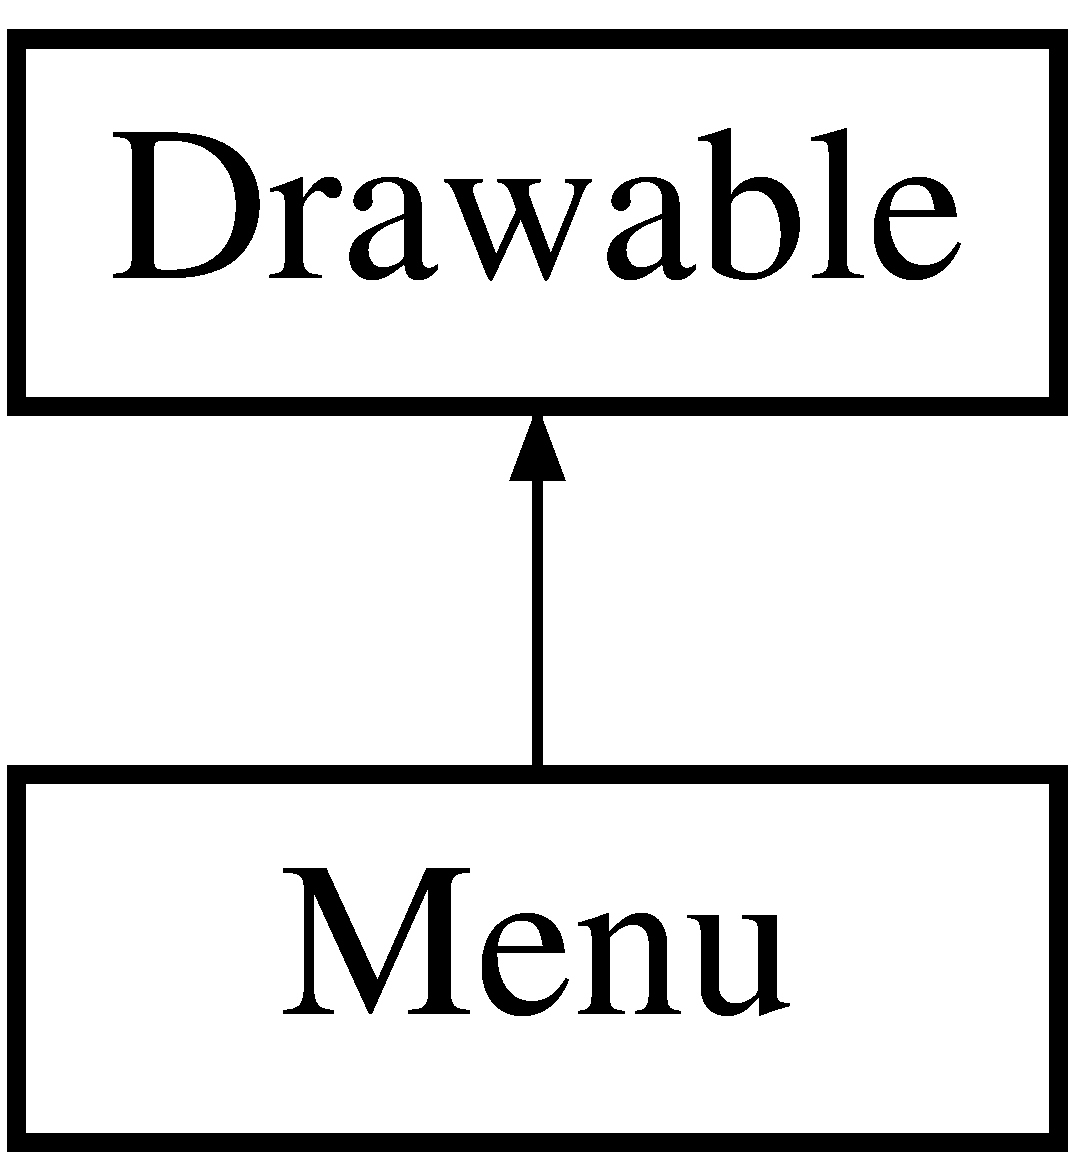
\includegraphics[height=2.000000cm]{class_menu}
\end{center}
\end{figure}
\subsection*{Metody publiczne}
\begin{DoxyCompactItemize}
\item 
\mbox{\hyperlink{class_menu_ad466dd83355124a6ed958430450bfe94}{Menu}} ()
\begin{DoxyCompactList}\small\item\em Konstruktor menu. \end{DoxyCompactList}\item 
\mbox{\hyperlink{class_button}{Button}} $\ast$ \mbox{\hyperlink{class_menu_add20f283775e3cdb3ad8e8f8f02af83e}{get\+Button}} (float x, float y)
\begin{DoxyCompactList}\small\item\em Zwraca wska�nik na przycisk o podanych wsp�rz�dnych. \end{DoxyCompactList}\item 
void \mbox{\hyperlink{class_menu_a6ebff4998eb64bad2871a658ab7ed3c0}{clear\+Clicked\+Button}} ()
\begin{DoxyCompactList}\small\item\em Czy�ci klikni�ty przycisk. \end{DoxyCompactList}\item 
void \mbox{\hyperlink{class_menu_a3630ce145aab68961ec535762d928558}{clear}} ()
\begin{DoxyCompactList}\small\item\em Czy�ci menu. \end{DoxyCompactList}\item 
void \mbox{\hyperlink{class_menu_a55609527292757ffa53fdfc6c2a23a38}{change\+Menu}} (int choice)
\begin{DoxyCompactList}\small\item\em Zmienia menu. \end{DoxyCompactList}\end{DoxyCompactItemize}
\subsection*{Metody chronione}
\begin{DoxyCompactItemize}
\item 
void \mbox{\hyperlink{class_menu_a0a6873f5c605195a1f242c3f678df55e}{draw}} (sf\+::\+Render\+Target \&target, sf\+::\+Render\+States states) const override
\begin{DoxyCompactList}\small\item\em Rysuje obiekt na ekranie (dzidziczona z S\+F\+ML) \end{DoxyCompactList}\end{DoxyCompactItemize}


\subsection{Opis szczegółowy}


Definicja w linii 7 pliku Menu.\+h.



\subsection{Dokumentacja konstruktora i destruktora}
\mbox{\Hypertarget{class_menu_ad466dd83355124a6ed958430450bfe94}\label{class_menu_ad466dd83355124a6ed958430450bfe94}} 
\index{Menu@{Menu}!Menu@{Menu}}
\index{Menu@{Menu}!Menu@{Menu}}
\subsubsection{\texorpdfstring{Menu()}{Menu()}}
{\footnotesize\ttfamily Menu\+::\+Menu (\begin{DoxyParamCaption}{ }\end{DoxyParamCaption})}



Konstruktor menu. 



Definicja w linii 6 pliku Menu.\+cpp.



\subsection{Dokumentacja funkcji składowych}
\mbox{\Hypertarget{class_menu_a55609527292757ffa53fdfc6c2a23a38}\label{class_menu_a55609527292757ffa53fdfc6c2a23a38}} 
\index{Menu@{Menu}!change\+Menu@{change\+Menu}}
\index{change\+Menu@{change\+Menu}!Menu@{Menu}}
\subsubsection{\texorpdfstring{change\+Menu()}{changeMenu()}}
{\footnotesize\ttfamily void Menu\+::change\+Menu (\begin{DoxyParamCaption}\item[{int}]{choice }\end{DoxyParamCaption})}



Zmienia menu. 


\begin{DoxyParams}{Parametry}
{\em choice} & -\/ wyb�r \\
\hline
\end{DoxyParams}


Definicja w linii 86 pliku Menu.\+cpp.

\mbox{\Hypertarget{class_menu_a3630ce145aab68961ec535762d928558}\label{class_menu_a3630ce145aab68961ec535762d928558}} 
\index{Menu@{Menu}!clear@{clear}}
\index{clear@{clear}!Menu@{Menu}}
\subsubsection{\texorpdfstring{clear()}{clear()}}
{\footnotesize\ttfamily void Menu\+::clear (\begin{DoxyParamCaption}{ }\end{DoxyParamCaption})}



Czy�ci menu. 



Definicja w linii 78 pliku Menu.\+cpp.

\mbox{\Hypertarget{class_menu_a6ebff4998eb64bad2871a658ab7ed3c0}\label{class_menu_a6ebff4998eb64bad2871a658ab7ed3c0}} 
\index{Menu@{Menu}!clear\+Clicked\+Button@{clear\+Clicked\+Button}}
\index{clear\+Clicked\+Button@{clear\+Clicked\+Button}!Menu@{Menu}}
\subsubsection{\texorpdfstring{clear\+Clicked\+Button()}{clearClickedButton()}}
{\footnotesize\ttfamily void Menu\+::clear\+Clicked\+Button (\begin{DoxyParamCaption}{ }\end{DoxyParamCaption})}



Czy�ci klikni�ty przycisk. 



Definicja w linii 68 pliku Menu.\+cpp.

\mbox{\Hypertarget{class_menu_a0a6873f5c605195a1f242c3f678df55e}\label{class_menu_a0a6873f5c605195a1f242c3f678df55e}} 
\index{Menu@{Menu}!draw@{draw}}
\index{draw@{draw}!Menu@{Menu}}
\subsubsection{\texorpdfstring{draw()}{draw()}}
{\footnotesize\ttfamily void Menu\+::draw (\begin{DoxyParamCaption}\item[{sf\+::\+Render\+Target \&}]{target,  }\item[{sf\+::\+Render\+States}]{states }\end{DoxyParamCaption}) const\hspace{0.3cm}{\ttfamily [override]}, {\ttfamily [protected]}}



Rysuje obiekt na ekranie (dzidziczona z S\+F\+ML) 


\begin{DoxyParams}{Parametry}
{\em target} & \\
\hline
{\em states} & \\
\hline
\end{DoxyParams}


Definicja w linii 30 pliku Menu.\+cpp.

\mbox{\Hypertarget{class_menu_add20f283775e3cdb3ad8e8f8f02af83e}\label{class_menu_add20f283775e3cdb3ad8e8f8f02af83e}} 
\index{Menu@{Menu}!get\+Button@{get\+Button}}
\index{get\+Button@{get\+Button}!Menu@{Menu}}
\subsubsection{\texorpdfstring{get\+Button()}{getButton()}}
{\footnotesize\ttfamily \mbox{\hyperlink{class_button}{Button}} $\ast$ Menu\+::get\+Button (\begin{DoxyParamCaption}\item[{float}]{x,  }\item[{float}]{y }\end{DoxyParamCaption})}



Zwraca wska�nik na przycisk o podanych wsp�rz�dnych. 


\begin{DoxyParams}{Parametry}
{\em x} & -\/ Wsp�rz�dna X przycisku \\
\hline
{\em y} & -\/ Wsp�rz�dna Y przycisku \\
\hline
\end{DoxyParams}
\begin{DoxyReturn}{Zwraca}
wska�nik na przycisk 
\end{DoxyReturn}


Definicja w linii 47 pliku Menu.\+cpp.



Dokumentacja dla tej klasy została wygenerowana z plików\+:\begin{DoxyCompactItemize}
\item 
D\+:/\+Projekty/\+C++/\+Programowanie w C2/\+Worms 2\+D/\+Worms 2\+D/\mbox{\hyperlink{_menu_8h}{Menu.\+h}}\item 
D\+:/\+Projekty/\+C++/\+Programowanie w C2/\+Worms 2\+D/\+Worms 2\+D/\mbox{\hyperlink{_menu_8cpp}{Menu.\+cpp}}\end{DoxyCompactItemize}

\hypertarget{class_revolver}{}\section{Dokumentacja klasy Revolver}
\label{class_revolver}\index{Revolver@{Revolver}}


Klasa rewolwera.  




{\ttfamily \#include $<$Revolver.\+h$>$}

Diagram dziedziczenia dla Revolver\begin{figure}[H]
\begin{center}
\leavevmode
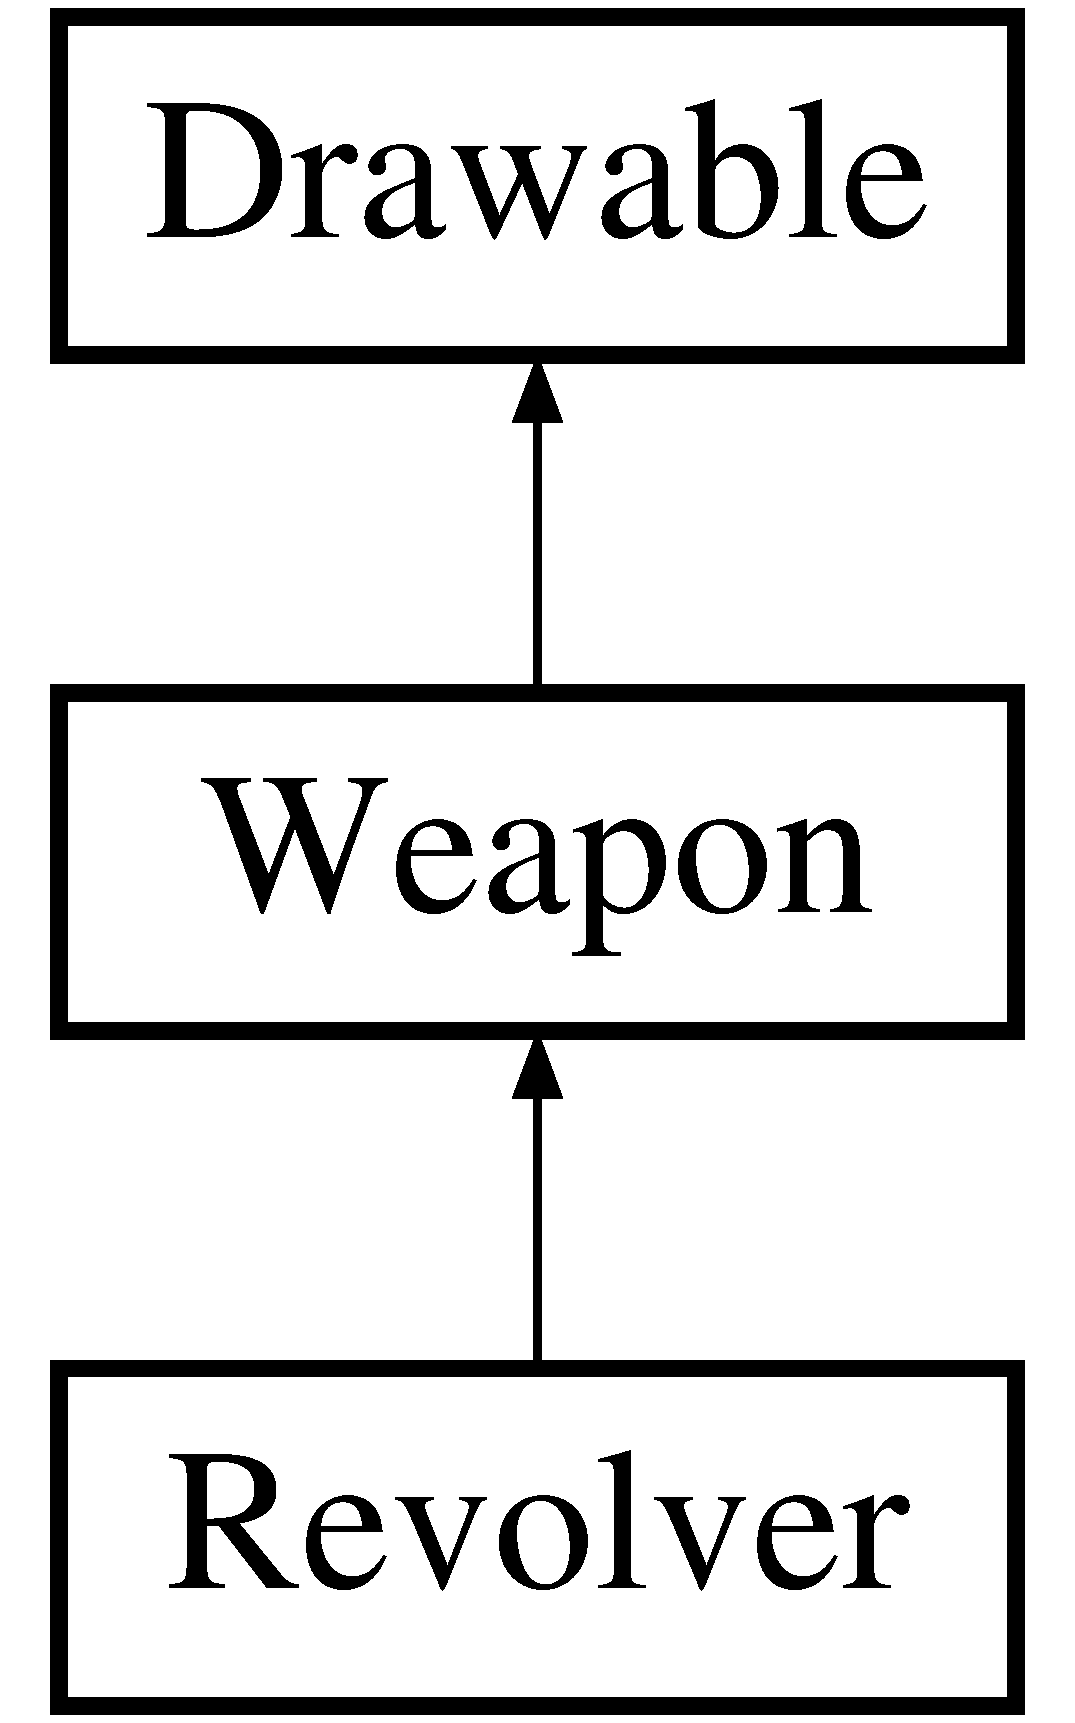
\includegraphics[height=3.000000cm]{class_revolver}
\end{center}
\end{figure}
\subsection*{Metody publiczne}
\begin{DoxyCompactItemize}
\item 
\mbox{\hyperlink{class_revolver_ab4d4360bde9164e0f697a7fe3f91d8aa}{Revolver}} ()=delete
\begin{DoxyCompactList}\small\item\em Konstruktor domyślny który jest usunięty. \end{DoxyCompactList}\item 
\mbox{\hyperlink{class_revolver_a91db226199031f40f2789321108e2569}{Revolver}} (float x, float y)
\begin{DoxyCompactList}\small\item\em Konstruktor broni. \end{DoxyCompactList}\item 
virtual \mbox{\hyperlink{class_revolver_a989391a89ed1babecbc7360d670f3bc8}{$\sim$\+Revolver}} ()=default
\begin{DoxyCompactList}\small\item\em Domyślny destruktor. \end{DoxyCompactList}\item 
void \mbox{\hyperlink{class_revolver_acc5cf142969078c7ee588582cd7c9316}{play\+Shoot\+Sound}} () override
\begin{DoxyCompactList}\small\item\em Przeciążona funkcja odtwarzająca odgłos wystrzału z broni. \end{DoxyCompactList}\end{DoxyCompactItemize}
\subsection*{Dodatkowe Dziedziczone Składowe}


\subsection{Opis szczegółowy}
Klasa rewolwera. 

Definicja w linii 7 pliku Revolver.\+h.



\subsection{Dokumentacja konstruktora i destruktora}
\mbox{\Hypertarget{class_revolver_ab4d4360bde9164e0f697a7fe3f91d8aa}\label{class_revolver_ab4d4360bde9164e0f697a7fe3f91d8aa}} 
\index{Revolver@{Revolver}!Revolver@{Revolver}}
\index{Revolver@{Revolver}!Revolver@{Revolver}}
\subsubsection{\texorpdfstring{Revolver()}{Revolver()}\hspace{0.1cm}{\footnotesize\ttfamily [1/2]}}
{\footnotesize\ttfamily Revolver\+::\+Revolver (\begin{DoxyParamCaption}{ }\end{DoxyParamCaption})\hspace{0.3cm}{\ttfamily [delete]}}



Konstruktor domyślny który jest usunięty. 

\mbox{\Hypertarget{class_revolver_a91db226199031f40f2789321108e2569}\label{class_revolver_a91db226199031f40f2789321108e2569}} 
\index{Revolver@{Revolver}!Revolver@{Revolver}}
\index{Revolver@{Revolver}!Revolver@{Revolver}}
\subsubsection{\texorpdfstring{Revolver()}{Revolver()}\hspace{0.1cm}{\footnotesize\ttfamily [2/2]}}
{\footnotesize\ttfamily Revolver\+::\+Revolver (\begin{DoxyParamCaption}\item[{float}]{x,  }\item[{float}]{y }\end{DoxyParamCaption})}



Konstruktor broni. 


\begin{DoxyParams}{Parametry}
{\em x} & -\/ współrzędna x wyświetlenia miejsca broni \\
\hline
{\em y} & -\/ współrzędna y wyświetlenia miejsca broni \\
\hline
\end{DoxyParams}


Definicja w linii 5 pliku Revolver.\+cpp.

\mbox{\Hypertarget{class_revolver_a989391a89ed1babecbc7360d670f3bc8}\label{class_revolver_a989391a89ed1babecbc7360d670f3bc8}} 
\index{Revolver@{Revolver}!````~Revolver@{$\sim$\+Revolver}}
\index{````~Revolver@{$\sim$\+Revolver}!Revolver@{Revolver}}
\subsubsection{\texorpdfstring{$\sim$\+Revolver()}{~Revolver()}}
{\footnotesize\ttfamily virtual Revolver\+::$\sim$\+Revolver (\begin{DoxyParamCaption}{ }\end{DoxyParamCaption})\hspace{0.3cm}{\ttfamily [virtual]}, {\ttfamily [default]}}



Domyślny destruktor. 



\subsection{Dokumentacja funkcji składowych}
\mbox{\Hypertarget{class_revolver_acc5cf142969078c7ee588582cd7c9316}\label{class_revolver_acc5cf142969078c7ee588582cd7c9316}} 
\index{Revolver@{Revolver}!play\+Shoot\+Sound@{play\+Shoot\+Sound}}
\index{play\+Shoot\+Sound@{play\+Shoot\+Sound}!Revolver@{Revolver}}
\subsubsection{\texorpdfstring{play\+Shoot\+Sound()}{playShootSound()}}
{\footnotesize\ttfamily void Revolver\+::play\+Shoot\+Sound (\begin{DoxyParamCaption}{ }\end{DoxyParamCaption})\hspace{0.3cm}{\ttfamily [override]}, {\ttfamily [virtual]}}



Przeciążona funkcja odtwarzająca odgłos wystrzału z broni. 



Reimplementowana z \mbox{\hyperlink{class_weapon_aaf32c85f3e70d3c8392c928b9e6e75ca}{Weapon}}.



Definicja w linii 16 pliku Revolver.\+cpp.



Dokumentacja dla tej klasy została wygenerowana z plików\+:\begin{DoxyCompactItemize}
\item 
D\+:/\+Projekty/\+C++/\+Programowanie w C2/\+Worms 2\+D/\+Worms 2\+D/\mbox{\hyperlink{_revolver_8h}{Revolver.\+h}}\item 
D\+:/\+Projekty/\+C++/\+Programowanie w C2/\+Worms 2\+D/\+Worms 2\+D/\mbox{\hyperlink{_revolver_8cpp}{Revolver.\+cpp}}\end{DoxyCompactItemize}

\hypertarget{class_terrain}{}\section{Dokumentacja klasy Terrain}
\label{class_terrain}\index{Terrain@{Terrain}}


{\ttfamily \#include $<$Terrain.\+h$>$}

Diagram dziedziczenia dla Terrain\begin{figure}[H]
\begin{center}
\leavevmode
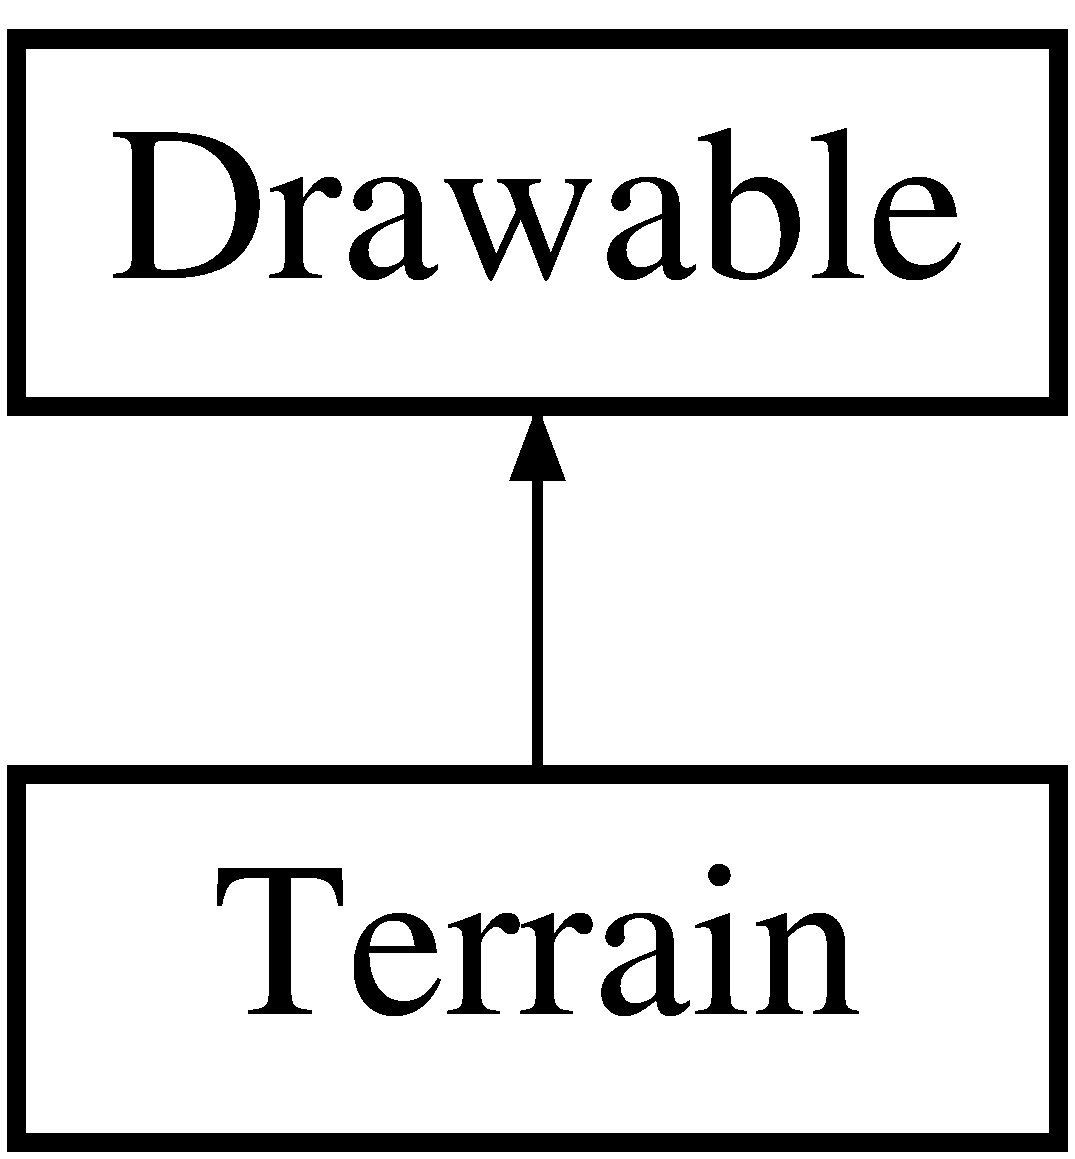
\includegraphics[height=2.000000cm]{class_terrain}
\end{center}
\end{figure}
\subsection*{Metody publiczne}
\begin{DoxyCompactItemize}
\item 
\mbox{\hyperlink{class_terrain_a7160a06ab07a86ed97d23374405e8ef6}{Terrain}} ()
\item 
void \mbox{\hyperlink{class_terrain_a552c55d3ce93ae1c8988432acdf7aea1}{erase}} (const sf\+::\+Drawable \&eraser)
\item 
void \mbox{\hyperlink{class_terrain_a009d97df85f0704ad9ea3c61fcd11080}{reset}} ()
\end{DoxyCompactItemize}
\subsection*{Atrybuty publiczne}
\begin{DoxyCompactItemize}
\item 
sf\+::\+Image \mbox{\hyperlink{class_terrain_afda7533fb267038f082301a417691483}{map}}
\end{DoxyCompactItemize}
\subsection*{Metody chronione}
\begin{DoxyCompactItemize}
\item 
void \mbox{\hyperlink{class_terrain_a78fb38a85917a89fa9deb9eec9599b49}{draw}} (sf\+::\+Render\+Target \&target, sf\+::\+Render\+States states) const override
\end{DoxyCompactItemize}


\subsection{Opis szczegółowy}


Definicja w linii 3 pliku Terrain.\+h.



\subsection{Dokumentacja konstruktora i destruktora}
\mbox{\Hypertarget{class_terrain_a7160a06ab07a86ed97d23374405e8ef6}\label{class_terrain_a7160a06ab07a86ed97d23374405e8ef6}} 
\index{Terrain@{Terrain}!Terrain@{Terrain}}
\index{Terrain@{Terrain}!Terrain@{Terrain}}
\subsubsection{\texorpdfstring{Terrain()}{Terrain()}}
{\footnotesize\ttfamily Terrain\+::\+Terrain (\begin{DoxyParamCaption}{ }\end{DoxyParamCaption})}



Definicja w linii 3 pliku Terrain.\+cpp.



\subsection{Dokumentacja funkcji składowych}
\mbox{\Hypertarget{class_terrain_a78fb38a85917a89fa9deb9eec9599b49}\label{class_terrain_a78fb38a85917a89fa9deb9eec9599b49}} 
\index{Terrain@{Terrain}!draw@{draw}}
\index{draw@{draw}!Terrain@{Terrain}}
\subsubsection{\texorpdfstring{draw()}{draw()}}
{\footnotesize\ttfamily void Terrain\+::draw (\begin{DoxyParamCaption}\item[{sf\+::\+Render\+Target \&}]{target,  }\item[{sf\+::\+Render\+States}]{states }\end{DoxyParamCaption}) const\hspace{0.3cm}{\ttfamily [override]}, {\ttfamily [protected]}}



Definicja w linii 31 pliku Terrain.\+cpp.

\mbox{\Hypertarget{class_terrain_a552c55d3ce93ae1c8988432acdf7aea1}\label{class_terrain_a552c55d3ce93ae1c8988432acdf7aea1}} 
\index{Terrain@{Terrain}!erase@{erase}}
\index{erase@{erase}!Terrain@{Terrain}}
\subsubsection{\texorpdfstring{erase()}{erase()}}
{\footnotesize\ttfamily void Terrain\+::erase (\begin{DoxyParamCaption}\item[{const sf\+::\+Drawable \&}]{eraser }\end{DoxyParamCaption})}



Definicja w linii 18 pliku Terrain.\+cpp.

\mbox{\Hypertarget{class_terrain_a009d97df85f0704ad9ea3c61fcd11080}\label{class_terrain_a009d97df85f0704ad9ea3c61fcd11080}} 
\index{Terrain@{Terrain}!reset@{reset}}
\index{reset@{reset}!Terrain@{Terrain}}
\subsubsection{\texorpdfstring{reset()}{reset()}}
{\footnotesize\ttfamily void Terrain\+::reset (\begin{DoxyParamCaption}{ }\end{DoxyParamCaption})}



Definicja w linii 37 pliku Terrain.\+cpp.



\subsection{Dokumentacja atrybutów składowych}
\mbox{\Hypertarget{class_terrain_afda7533fb267038f082301a417691483}\label{class_terrain_afda7533fb267038f082301a417691483}} 
\index{Terrain@{Terrain}!map@{map}}
\index{map@{map}!Terrain@{Terrain}}
\subsubsection{\texorpdfstring{map}{map}}
{\footnotesize\ttfamily sf\+::\+Image Terrain\+::map}



Definicja w linii 9 pliku Terrain.\+h.



Dokumentacja dla tej klasy została wygenerowana z plików\+:\begin{DoxyCompactItemize}
\item 
D\+:/\+Projekty/\+C++/\+Programowanie w C2/\+Worms 2\+D/\+Worms 2\+D/\mbox{\hyperlink{_terrain_8h}{Terrain.\+h}}\item 
D\+:/\+Projekty/\+C++/\+Programowanie w C2/\+Worms 2\+D/\+Worms 2\+D/\mbox{\hyperlink{_terrain_8cpp}{Terrain.\+cpp}}\end{DoxyCompactItemize}

\hypertarget{class_water}{}\section{Dokumentacja klasy Water}
\label{class_water}\index{Water@{Water}}


{\ttfamily \#include $<$Water.\+h$>$}

Diagram dziedziczenia dla Water\begin{figure}[H]
\begin{center}
\leavevmode
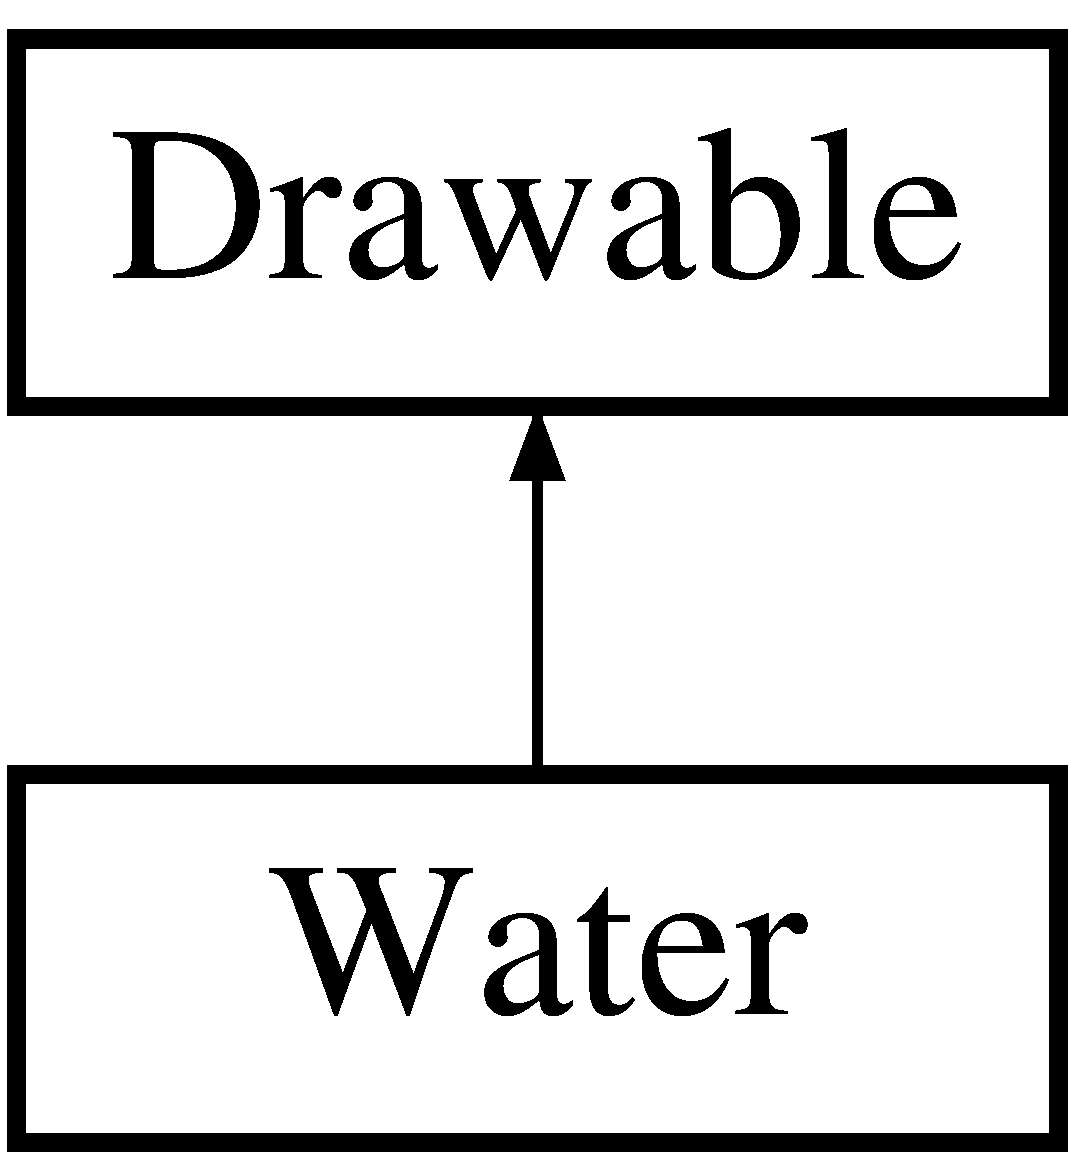
\includegraphics[height=2.000000cm]{class_water}
\end{center}
\end{figure}
\subsection*{Metody publiczne}
\begin{DoxyCompactItemize}
\item 
\mbox{\hyperlink{class_water_a32d8f391b149a405008a606ceafa35ee}{Water}} ()
\item 
void \mbox{\hyperlink{class_water_a18fce2c0b2c45ee4ea8e413fcb4bdafa}{update}} ()
\end{DoxyCompactItemize}
\subsection*{Metody chronione}
\begin{DoxyCompactItemize}
\item 
void \mbox{\hyperlink{class_water_a4a929b9c339c55d6c7bcabe79349bae8}{draw}} (sf\+::\+Render\+Target \&target, sf\+::\+Render\+States states) const override
\end{DoxyCompactItemize}


\subsection{Opis szczegółowy}


Definicja w linii 3 pliku Water.\+h.



\subsection{Dokumentacja konstruktora i destruktora}
\mbox{\Hypertarget{class_water_a32d8f391b149a405008a606ceafa35ee}\label{class_water_a32d8f391b149a405008a606ceafa35ee}} 
\index{Water@{Water}!Water@{Water}}
\index{Water@{Water}!Water@{Water}}
\subsubsection{\texorpdfstring{Water()}{Water()}}
{\footnotesize\ttfamily Water\+::\+Water (\begin{DoxyParamCaption}{ }\end{DoxyParamCaption})}



Definicja w linii 2 pliku Water.\+cpp.



\subsection{Dokumentacja funkcji składowych}
\mbox{\Hypertarget{class_water_a4a929b9c339c55d6c7bcabe79349bae8}\label{class_water_a4a929b9c339c55d6c7bcabe79349bae8}} 
\index{Water@{Water}!draw@{draw}}
\index{draw@{draw}!Water@{Water}}
\subsubsection{\texorpdfstring{draw()}{draw()}}
{\footnotesize\ttfamily void Water\+::draw (\begin{DoxyParamCaption}\item[{sf\+::\+Render\+Target \&}]{target,  }\item[{sf\+::\+Render\+States}]{states }\end{DoxyParamCaption}) const\hspace{0.3cm}{\ttfamily [override]}, {\ttfamily [protected]}}



Definicja w linii 64 pliku Water.\+cpp.

\mbox{\Hypertarget{class_water_a18fce2c0b2c45ee4ea8e413fcb4bdafa}\label{class_water_a18fce2c0b2c45ee4ea8e413fcb4bdafa}} 
\index{Water@{Water}!update@{update}}
\index{update@{update}!Water@{Water}}
\subsubsection{\texorpdfstring{update()}{update()}}
{\footnotesize\ttfamily void Water\+::update (\begin{DoxyParamCaption}{ }\end{DoxyParamCaption})}



Definicja w linii 35 pliku Water.\+cpp.



Dokumentacja dla tej klasy została wygenerowana z plików\+:\begin{DoxyCompactItemize}
\item 
D\+:/\+Projekty/\+C++/\+Programowanie w C2/\+Worms 2\+D/\+Worms 2\+D/\mbox{\hyperlink{_water_8h}{Water.\+h}}\item 
D\+:/\+Projekty/\+C++/\+Programowanie w C2/\+Worms 2\+D/\+Worms 2\+D/\mbox{\hyperlink{_water_8cpp}{Water.\+cpp}}\end{DoxyCompactItemize}

\hypertarget{class_weapon}{}\section{Dokumentacja klasy Weapon}
\label{class_weapon}\index{Weapon@{Weapon}}


Klasa bazowa broni.  




{\ttfamily \#include $<$Weapon.\+h$>$}

Diagram dziedziczenia dla Weapon\begin{figure}[H]
\begin{center}
\leavevmode
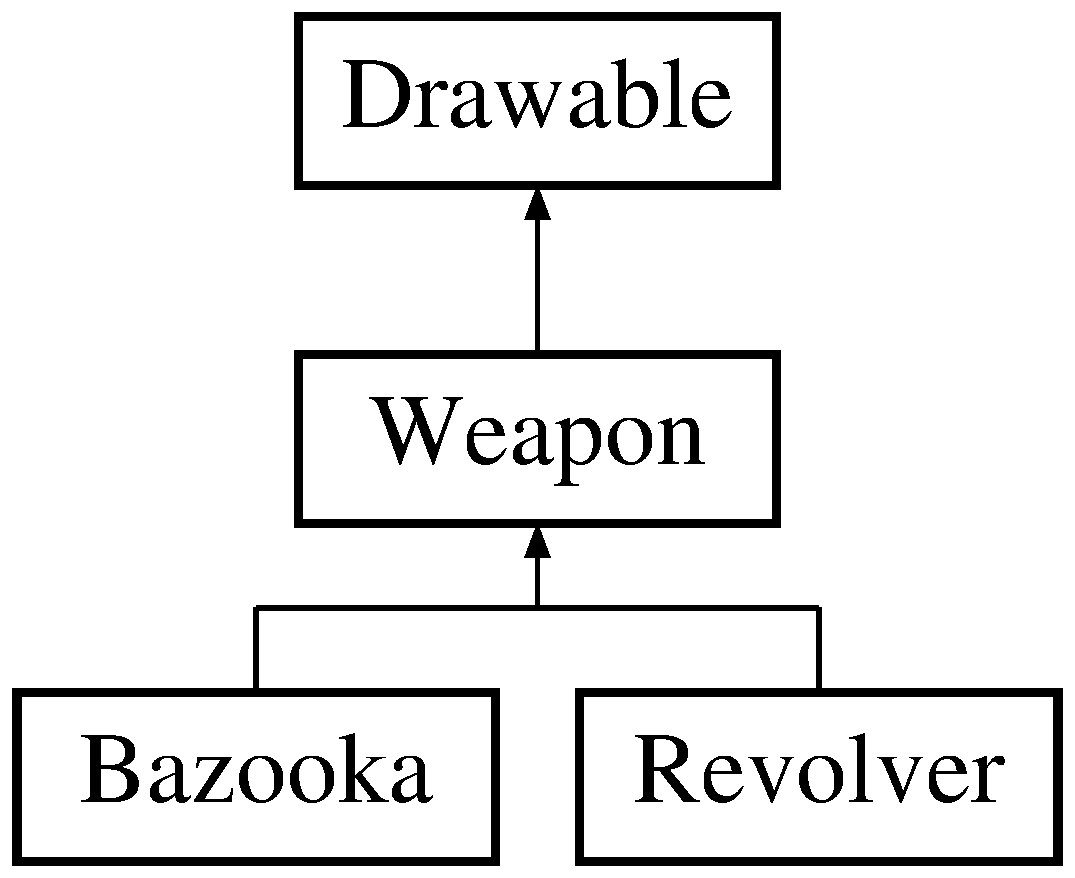
\includegraphics[height=3.000000cm]{class_weapon}
\end{center}
\end{figure}
\subsection*{Metody publiczne}
\begin{DoxyCompactItemize}
\item 
\mbox{\hyperlink{class_weapon_afe032e854c543fe393fda4e3e6b9fafc}{Weapon}} ()=delete
\begin{DoxyCompactList}\small\item\em Konstruktor domyślny broni który jest usunięty. \end{DoxyCompactList}\item 
\mbox{\hyperlink{class_weapon_a0640cf23068ebf732ce564329e5c40f4}{Weapon}} (float x, float y)
\begin{DoxyCompactList}\small\item\em Konstruktor broni. \end{DoxyCompactList}\item 
virtual \mbox{\hyperlink{class_weapon_af06462587d8fd8878be4af2a2479f9bb}{$\sim$\+Weapon}} ()=default
\begin{DoxyCompactList}\small\item\em Domyślny destruktor wirtualny broni. \end{DoxyCompactList}\item 
void \mbox{\hyperlink{class_weapon_ae7f10f6f35f5b1cc4e073530841ade5d}{set\+Scale}} (float \mbox{\hyperlink{class_weapon_a425a9f9fc4bb9bf0e4de80855d3e2ac0}{scale}})
\begin{DoxyCompactList}\small\item\em Metoda ustawiająca skale broni. \end{DoxyCompactList}\item 
void \mbox{\hyperlink{class_weapon_a057b4129e261b70f3a12703e475da353}{set\+Rotation}} (float \mbox{\hyperlink{class_weapon_aea591386a659ecf7dd7e41ada97db990}{rotation}})
\begin{DoxyCompactList}\small\item\em Metoda ustawiająca rotacje broni. \end{DoxyCompactList}\item 
float \mbox{\hyperlink{class_weapon_ac7ab3d1fc902d0a063d5c447ebda674b}{get\+Scale}} () const
\begin{DoxyCompactList}\small\item\em Metoda zwracająca skale broni. \end{DoxyCompactList}\item 
float \mbox{\hyperlink{class_weapon_af16afbd2da86bee0e48680e962abeca5}{get\+Rotation}} () const
\begin{DoxyCompactList}\small\item\em Metoda zwracająca rotacje broni. \end{DoxyCompactList}\item 
sf\+::\+Sprite \mbox{\hyperlink{class_weapon_a1da4c7c6528d560e2a183ecd6e65d27b}{get\+Sprite}} () const
\begin{DoxyCompactList}\small\item\em Metoda zwracająca obiekt sprite\textquotesingle{}a broni. \end{DoxyCompactList}\item 
float \mbox{\hyperlink{class_weapon_ac46e15594ab133d8bd9484f31675c087}{get\+PosX}} () const
\begin{DoxyCompactList}\small\item\em Zwraca wspołrzędną X broni. \end{DoxyCompactList}\item 
float \mbox{\hyperlink{class_weapon_a725696ea526b49b35b4219fdd7faa68e}{get\+PosY}} () const
\begin{DoxyCompactList}\small\item\em Zwraca współrzędną Y broni. \end{DoxyCompactList}\item 
void \mbox{\hyperlink{class_weapon_a889af631d759a2911045d699d6801623}{set\+PosX}} (float x)
\begin{DoxyCompactList}\small\item\em Ustawia współrzędną X broni. \end{DoxyCompactList}\item 
void \mbox{\hyperlink{class_weapon_acd2619f9d9d417cf655d53149ee53540}{set\+PosY}} (float y)
\begin{DoxyCompactList}\small\item\em Ustawia współrzedną Y broni. \end{DoxyCompactList}\item 
void \mbox{\hyperlink{class_weapon_addd624ea7d811b1bf61c2abb4a812f87}{set\+Bullet}} (\mbox{\hyperlink{class_bullet}{Bullet}} $\ast$\mbox{\hyperlink{class_weapon_a799874e40f4d2235ffa259eb46674fe5}{bullet}})
\begin{DoxyCompactList}\small\item\em Ustawia pocisk broni na wskazany w parametrze obiekt. \end{DoxyCompactList}\item 
void \mbox{\hyperlink{class_weapon_afc47346b4e4f0f41599fdaec6c47ae6d}{set\+Scale\+Vector}} (sf\+::\+Vector2f \mbox{\hyperlink{class_weapon_a425a9f9fc4bb9bf0e4de80855d3e2ac0}{scale}})
\begin{DoxyCompactList}\small\item\em Ustawia wektor skali broni. \end{DoxyCompactList}\item 
sf\+::\+Vector2f \mbox{\hyperlink{class_weapon_a91adf453c2d656f577686b31d1f87e25}{get\+Scale\+Vector}} () const
\begin{DoxyCompactList}\small\item\em Zwraca wektor skali broni. \end{DoxyCompactList}\item 
\mbox{\hyperlink{class_bullet}{Bullet}} $\ast$ \mbox{\hyperlink{class_weapon_a9cf68e4a72e5513266ca3e59f48da323}{get\+Bullet}} ()
\begin{DoxyCompactList}\small\item\em Zwraca wskaźnik na obiekt pocisku danej broni. \end{DoxyCompactList}\item 
void \mbox{\hyperlink{class_weapon_a1b3f76c5275b67f0bb8073157a27e736}{update}} ()
\begin{DoxyCompactList}\small\item\em Metoda aktualizująca obiekt broni co klatke. \end{DoxyCompactList}\item 
virtual void \mbox{\hyperlink{class_weapon_a954c06c805704aeea451f88221e5c74c}{shoot}} (float angle)
\begin{DoxyCompactList}\small\item\em Wirtualna metoda sprawiająca, że broń wystrzeli. \end{DoxyCompactList}\item 
bool \mbox{\hyperlink{class_weapon_a71c1102f1e752307efbb83c7140bca66}{get\+Is\+Shooting}} () const
\begin{DoxyCompactList}\small\item\em Zwraca wartość informującą o tym czy broń aktualnie strzela. \end{DoxyCompactList}\item 
void \mbox{\hyperlink{class_weapon_abadbad398e52fb1ef6364cd2e0d2defb}{set\+Is\+Shooting}} (bool \mbox{\hyperlink{class_weapon_aa546d4d559c3fe1d7aefa13f62eb2890}{is\+Shooting}})
\begin{DoxyCompactList}\small\item\em Ustawia stan strzelania broni na podany w parametrze. \end{DoxyCompactList}\item 
virtual void \mbox{\hyperlink{class_weapon_aaf32c85f3e70d3c8392c928b9e6e75ca}{play\+Shoot\+Sound}} ()
\begin{DoxyCompactList}\small\item\em Odtwarza dźwięk wystrzału broni. \end{DoxyCompactList}\item 
void \mbox{\hyperlink{class_weapon_a00809195a729c5efc854a0fe6dda72aa}{set\+Damage}} (float \mbox{\hyperlink{class_weapon_a5fd71198c35ebc63e9d5c4fc486d2510}{damage}})
\begin{DoxyCompactList}\small\item\em Ustawia obrażenia od danej broni. \end{DoxyCompactList}\item 
float \mbox{\hyperlink{class_weapon_a35dc33e086bd053d95b10d4a7c83494c}{get\+Damage}} () const
\begin{DoxyCompactList}\small\item\em Zwraca obrażenia danej broni. \end{DoxyCompactList}\end{DoxyCompactItemize}
\subsection*{Metody chronione}
\begin{DoxyCompactItemize}
\item 
void \mbox{\hyperlink{class_weapon_ae0cdebb7e5fde5a913a390ff573001e2}{draw}} (sf\+::\+Render\+Target \&target, sf\+::\+Render\+States states) const override
\begin{DoxyCompactList}\small\item\em Rysuje obiekt na ekranie (dzidziczona z S\+F\+ML) \end{DoxyCompactList}\end{DoxyCompactItemize}
\subsection*{Atrybuty chronione}
\begin{DoxyCompactItemize}
\item 
sf\+::\+Sprite \mbox{\hyperlink{class_weapon_ad56c11bff999e073bf880d482d54e06b}{sprite}}
\begin{DoxyCompactList}\small\item\em Obiekt rysowany na ekranie. \end{DoxyCompactList}\item 
sf\+::\+Texture \mbox{\hyperlink{class_weapon_a57095692a0468a109bba97fbd8c25db5}{texture}}
\begin{DoxyCompactList}\small\item\em Tekstura obiektu. \end{DoxyCompactList}\item 
std\+::string \mbox{\hyperlink{class_weapon_a340a6850f1bbf30d874aede653c249a9}{texture\+Path}}
\begin{DoxyCompactList}\small\item\em Ścieżka do tekstury obiektu. \end{DoxyCompactList}\item 
\mbox{\hyperlink{class_bullet}{Bullet}} $\ast$ \mbox{\hyperlink{class_weapon_a799874e40f4d2235ffa259eb46674fe5}{bullet}} = nullptr
\item 
float \mbox{\hyperlink{class_weapon_aea591386a659ecf7dd7e41ada97db990}{rotation}} = 0.\+0f
\begin{DoxyCompactList}\small\item\em Wartość rotacji broni. \end{DoxyCompactList}\item 
float \mbox{\hyperlink{class_weapon_a425a9f9fc4bb9bf0e4de80855d3e2ac0}{scale}} = 0.\+2f
\begin{DoxyCompactList}\small\item\em Wartość skali broni. \end{DoxyCompactList}\item 
float \mbox{\hyperlink{class_weapon_a977cf65797ba61f2b8cba78a6cd6adfa}{posX}}
\begin{DoxyCompactList}\small\item\em Pozycja X broni na ekranie. \end{DoxyCompactList}\item 
float \mbox{\hyperlink{class_weapon_a17ab9aa81f8c4476b43a8f71cd93a994}{posY}}
\begin{DoxyCompactList}\small\item\em Pozycja Y broni na ekranie. \end{DoxyCompactList}\item 
sf\+::\+Vector2f \mbox{\hyperlink{class_weapon_a8783dd00b0d4281cf384f58db5f488b1}{scale\+Vector}} = \{ \mbox{\hyperlink{class_weapon_a425a9f9fc4bb9bf0e4de80855d3e2ac0}{scale}},\mbox{\hyperlink{class_weapon_a425a9f9fc4bb9bf0e4de80855d3e2ac0}{scale}} \}
\begin{DoxyCompactList}\small\item\em Wektor skali broni. \end{DoxyCompactList}\item 
bool \mbox{\hyperlink{class_weapon_aa546d4d559c3fe1d7aefa13f62eb2890}{is\+Shooting}} = false
\begin{DoxyCompactList}\small\item\em Przechowuje informacje o tym czy broń strzela. \end{DoxyCompactList}\item 
float \mbox{\hyperlink{class_weapon_a5fd71198c35ebc63e9d5c4fc486d2510}{damage}} = 0.\+0f
\begin{DoxyCompactList}\small\item\em Obrażenia broni. \end{DoxyCompactList}\end{DoxyCompactItemize}


\subsection{Opis szczegółowy}
Klasa bazowa broni. 

Definicja w linii 12 pliku Weapon.\+h.



\subsection{Dokumentacja konstruktora i destruktora}
\mbox{\Hypertarget{class_weapon_afe032e854c543fe393fda4e3e6b9fafc}\label{class_weapon_afe032e854c543fe393fda4e3e6b9fafc}} 
\index{Weapon@{Weapon}!Weapon@{Weapon}}
\index{Weapon@{Weapon}!Weapon@{Weapon}}
\subsubsection{\texorpdfstring{Weapon()}{Weapon()}\hspace{0.1cm}{\footnotesize\ttfamily [1/2]}}
{\footnotesize\ttfamily Weapon\+::\+Weapon (\begin{DoxyParamCaption}{ }\end{DoxyParamCaption})\hspace{0.3cm}{\ttfamily [delete]}}



Konstruktor domyślny broni który jest usunięty. 

\mbox{\Hypertarget{class_weapon_a0640cf23068ebf732ce564329e5c40f4}\label{class_weapon_a0640cf23068ebf732ce564329e5c40f4}} 
\index{Weapon@{Weapon}!Weapon@{Weapon}}
\index{Weapon@{Weapon}!Weapon@{Weapon}}
\subsubsection{\texorpdfstring{Weapon()}{Weapon()}\hspace{0.1cm}{\footnotesize\ttfamily [2/2]}}
{\footnotesize\ttfamily Weapon\+::\+Weapon (\begin{DoxyParamCaption}\item[{float}]{x,  }\item[{float}]{y }\end{DoxyParamCaption})}



Konstruktor broni. 


\begin{DoxyParams}{Parametry}
{\em x} & -\/ współrzędna x wyświetlenia miejsca broni \\
\hline
{\em y} & -\/ współrzędna y wyświetlenia miejsca broni \\
\hline
\end{DoxyParams}


Definicja w linii 4 pliku Weapon.\+cpp.

\mbox{\Hypertarget{class_weapon_af06462587d8fd8878be4af2a2479f9bb}\label{class_weapon_af06462587d8fd8878be4af2a2479f9bb}} 
\index{Weapon@{Weapon}!````~Weapon@{$\sim$\+Weapon}}
\index{````~Weapon@{$\sim$\+Weapon}!Weapon@{Weapon}}
\subsubsection{\texorpdfstring{$\sim$\+Weapon()}{~Weapon()}}
{\footnotesize\ttfamily virtual Weapon\+::$\sim$\+Weapon (\begin{DoxyParamCaption}{ }\end{DoxyParamCaption})\hspace{0.3cm}{\ttfamily [virtual]}, {\ttfamily [default]}}



Domyślny destruktor wirtualny broni. 



\subsection{Dokumentacja funkcji składowych}
\mbox{\Hypertarget{class_weapon_ae0cdebb7e5fde5a913a390ff573001e2}\label{class_weapon_ae0cdebb7e5fde5a913a390ff573001e2}} 
\index{Weapon@{Weapon}!draw@{draw}}
\index{draw@{draw}!Weapon@{Weapon}}
\subsubsection{\texorpdfstring{draw()}{draw()}}
{\footnotesize\ttfamily void Weapon\+::draw (\begin{DoxyParamCaption}\item[{sf\+::\+Render\+Target \&}]{target,  }\item[{sf\+::\+Render\+States}]{states }\end{DoxyParamCaption}) const\hspace{0.3cm}{\ttfamily [override]}, {\ttfamily [protected]}}



Rysuje obiekt na ekranie (dzidziczona z S\+F\+ML) 


\begin{DoxyParams}{Parametry}
{\em target} & \\
\hline
{\em states} & \\
\hline
\end{DoxyParams}


Definicja w linii 131 pliku Weapon.\+cpp.

\mbox{\Hypertarget{class_weapon_a9cf68e4a72e5513266ca3e59f48da323}\label{class_weapon_a9cf68e4a72e5513266ca3e59f48da323}} 
\index{Weapon@{Weapon}!get\+Bullet@{get\+Bullet}}
\index{get\+Bullet@{get\+Bullet}!Weapon@{Weapon}}
\subsubsection{\texorpdfstring{get\+Bullet()}{getBullet()}}
{\footnotesize\ttfamily \mbox{\hyperlink{class_bullet}{Bullet}} $\ast$ Weapon\+::get\+Bullet (\begin{DoxyParamCaption}{ }\end{DoxyParamCaption})}



Zwraca wskaźnik na obiekt pocisku danej broni. 

\begin{DoxyReturn}{Zwraca}
Wskaźnik obiekt pocisku danej broni 
\end{DoxyReturn}


Definicja w linii 75 pliku Weapon.\+cpp.

\mbox{\Hypertarget{class_weapon_a35dc33e086bd053d95b10d4a7c83494c}\label{class_weapon_a35dc33e086bd053d95b10d4a7c83494c}} 
\index{Weapon@{Weapon}!get\+Damage@{get\+Damage}}
\index{get\+Damage@{get\+Damage}!Weapon@{Weapon}}
\subsubsection{\texorpdfstring{get\+Damage()}{getDamage()}}
{\footnotesize\ttfamily float Weapon\+::get\+Damage (\begin{DoxyParamCaption}{ }\end{DoxyParamCaption}) const}



Zwraca obrażenia danej broni. 

\begin{DoxyReturn}{Zwraca}
obrażenia broni 
\end{DoxyReturn}


Definicja w linii 126 pliku Weapon.\+cpp.

\mbox{\Hypertarget{class_weapon_a71c1102f1e752307efbb83c7140bca66}\label{class_weapon_a71c1102f1e752307efbb83c7140bca66}} 
\index{Weapon@{Weapon}!get\+Is\+Shooting@{get\+Is\+Shooting}}
\index{get\+Is\+Shooting@{get\+Is\+Shooting}!Weapon@{Weapon}}
\subsubsection{\texorpdfstring{get\+Is\+Shooting()}{getIsShooting()}}
{\footnotesize\ttfamily bool Weapon\+::get\+Is\+Shooting (\begin{DoxyParamCaption}{ }\end{DoxyParamCaption}) const}



Zwraca wartość informującą o tym czy broń aktualnie strzela. 

\begin{DoxyReturn}{Zwraca}
wartość informującą o tym czy broń aktualnie strzela 
\end{DoxyReturn}


Definicja w linii 107 pliku Weapon.\+cpp.

\mbox{\Hypertarget{class_weapon_ac46e15594ab133d8bd9484f31675c087}\label{class_weapon_ac46e15594ab133d8bd9484f31675c087}} 
\index{Weapon@{Weapon}!get\+PosX@{get\+PosX}}
\index{get\+PosX@{get\+PosX}!Weapon@{Weapon}}
\subsubsection{\texorpdfstring{get\+Pos\+X()}{getPosX()}}
{\footnotesize\ttfamily float Weapon\+::get\+PosX (\begin{DoxyParamCaption}{ }\end{DoxyParamCaption}) const}



Zwraca wspołrzędną X broni. 

\begin{DoxyReturn}{Zwraca}
współrzędną X broni 
\end{DoxyReturn}


Definicja w linii 40 pliku Weapon.\+cpp.

\mbox{\Hypertarget{class_weapon_a725696ea526b49b35b4219fdd7faa68e}\label{class_weapon_a725696ea526b49b35b4219fdd7faa68e}} 
\index{Weapon@{Weapon}!get\+PosY@{get\+PosY}}
\index{get\+PosY@{get\+PosY}!Weapon@{Weapon}}
\subsubsection{\texorpdfstring{get\+Pos\+Y()}{getPosY()}}
{\footnotesize\ttfamily float Weapon\+::get\+PosY (\begin{DoxyParamCaption}{ }\end{DoxyParamCaption}) const}



Zwraca współrzędną Y broni. 

\begin{DoxyReturn}{Zwraca}
współrzędną Y broni 
\end{DoxyReturn}


Definicja w linii 45 pliku Weapon.\+cpp.

\mbox{\Hypertarget{class_weapon_af16afbd2da86bee0e48680e962abeca5}\label{class_weapon_af16afbd2da86bee0e48680e962abeca5}} 
\index{Weapon@{Weapon}!get\+Rotation@{get\+Rotation}}
\index{get\+Rotation@{get\+Rotation}!Weapon@{Weapon}}
\subsubsection{\texorpdfstring{get\+Rotation()}{getRotation()}}
{\footnotesize\ttfamily float Weapon\+::get\+Rotation (\begin{DoxyParamCaption}{ }\end{DoxyParamCaption}) const}



Metoda zwracająca rotacje broni. 

\begin{DoxyReturn}{Zwraca}
Zwraca rotacje broni jako float 
\end{DoxyReturn}


Definicja w linii 30 pliku Weapon.\+cpp.

\mbox{\Hypertarget{class_weapon_ac7ab3d1fc902d0a063d5c447ebda674b}\label{class_weapon_ac7ab3d1fc902d0a063d5c447ebda674b}} 
\index{Weapon@{Weapon}!get\+Scale@{get\+Scale}}
\index{get\+Scale@{get\+Scale}!Weapon@{Weapon}}
\subsubsection{\texorpdfstring{get\+Scale()}{getScale()}}
{\footnotesize\ttfamily float Weapon\+::get\+Scale (\begin{DoxyParamCaption}{ }\end{DoxyParamCaption}) const}



Metoda zwracająca skale broni. 

\begin{DoxyReturn}{Zwraca}
Zwraca skale broni 
\end{DoxyReturn}


Definicja w linii 25 pliku Weapon.\+cpp.

\mbox{\Hypertarget{class_weapon_a91adf453c2d656f577686b31d1f87e25}\label{class_weapon_a91adf453c2d656f577686b31d1f87e25}} 
\index{Weapon@{Weapon}!get\+Scale\+Vector@{get\+Scale\+Vector}}
\index{get\+Scale\+Vector@{get\+Scale\+Vector}!Weapon@{Weapon}}
\subsubsection{\texorpdfstring{get\+Scale\+Vector()}{getScaleVector()}}
{\footnotesize\ttfamily sf\+::\+Vector2f Weapon\+::get\+Scale\+Vector (\begin{DoxyParamCaption}{ }\end{DoxyParamCaption}) const}



Zwraca wektor skali broni. 

\begin{DoxyReturn}{Zwraca}
Wektor skali broni 
\end{DoxyReturn}


Definicja w linii 70 pliku Weapon.\+cpp.

\mbox{\Hypertarget{class_weapon_a1da4c7c6528d560e2a183ecd6e65d27b}\label{class_weapon_a1da4c7c6528d560e2a183ecd6e65d27b}} 
\index{Weapon@{Weapon}!get\+Sprite@{get\+Sprite}}
\index{get\+Sprite@{get\+Sprite}!Weapon@{Weapon}}
\subsubsection{\texorpdfstring{get\+Sprite()}{getSprite()}}
{\footnotesize\ttfamily sf\+::\+Sprite Weapon\+::get\+Sprite (\begin{DoxyParamCaption}{ }\end{DoxyParamCaption}) const}



Metoda zwracająca obiekt sprite\textquotesingle{}a broni. 

\begin{DoxyReturn}{Zwraca}
obiekt sf\+::\+Sprite broni 
\end{DoxyReturn}


Definicja w linii 35 pliku Weapon.\+cpp.

\mbox{\Hypertarget{class_weapon_aaf32c85f3e70d3c8392c928b9e6e75ca}\label{class_weapon_aaf32c85f3e70d3c8392c928b9e6e75ca}} 
\index{Weapon@{Weapon}!play\+Shoot\+Sound@{play\+Shoot\+Sound}}
\index{play\+Shoot\+Sound@{play\+Shoot\+Sound}!Weapon@{Weapon}}
\subsubsection{\texorpdfstring{play\+Shoot\+Sound()}{playShootSound()}}
{\footnotesize\ttfamily void Weapon\+::play\+Shoot\+Sound (\begin{DoxyParamCaption}{ }\end{DoxyParamCaption})\hspace{0.3cm}{\ttfamily [virtual]}}



Odtwarza dźwięk wystrzału broni. 



Reimplementowana w \mbox{\hyperlink{class_bazooka_a2645b8043766ec5045e82d452828acdd}{Bazooka}} i \mbox{\hyperlink{class_revolver_acc5cf142969078c7ee588582cd7c9316}{Revolver}}.



Definicja w linii 117 pliku Weapon.\+cpp.

\mbox{\Hypertarget{class_weapon_addd624ea7d811b1bf61c2abb4a812f87}\label{class_weapon_addd624ea7d811b1bf61c2abb4a812f87}} 
\index{Weapon@{Weapon}!set\+Bullet@{set\+Bullet}}
\index{set\+Bullet@{set\+Bullet}!Weapon@{Weapon}}
\subsubsection{\texorpdfstring{set\+Bullet()}{setBullet()}}
{\footnotesize\ttfamily void Weapon\+::set\+Bullet (\begin{DoxyParamCaption}\item[{\mbox{\hyperlink{class_bullet}{Bullet}} $\ast$}]{bullet }\end{DoxyParamCaption})}



Ustawia pocisk broni na wskazany w parametrze obiekt. 


\begin{DoxyParams}{Parametry}
{\em bullet} & -\/ wskaźnik na obiekt pocisku \\
\hline
\end{DoxyParams}


Definicja w linii 60 pliku Weapon.\+cpp.

\mbox{\Hypertarget{class_weapon_a00809195a729c5efc854a0fe6dda72aa}\label{class_weapon_a00809195a729c5efc854a0fe6dda72aa}} 
\index{Weapon@{Weapon}!set\+Damage@{set\+Damage}}
\index{set\+Damage@{set\+Damage}!Weapon@{Weapon}}
\subsubsection{\texorpdfstring{set\+Damage()}{setDamage()}}
{\footnotesize\ttfamily void Weapon\+::set\+Damage (\begin{DoxyParamCaption}\item[{float}]{damage }\end{DoxyParamCaption})}



Ustawia obrażenia od danej broni. 


\begin{DoxyParams}{Parametry}
{\em damage} & -\/ obrażenia broni \\
\hline
\end{DoxyParams}


Definicja w linii 121 pliku Weapon.\+cpp.

\mbox{\Hypertarget{class_weapon_abadbad398e52fb1ef6364cd2e0d2defb}\label{class_weapon_abadbad398e52fb1ef6364cd2e0d2defb}} 
\index{Weapon@{Weapon}!set\+Is\+Shooting@{set\+Is\+Shooting}}
\index{set\+Is\+Shooting@{set\+Is\+Shooting}!Weapon@{Weapon}}
\subsubsection{\texorpdfstring{set\+Is\+Shooting()}{setIsShooting()}}
{\footnotesize\ttfamily void Weapon\+::set\+Is\+Shooting (\begin{DoxyParamCaption}\item[{bool}]{is\+Shooting }\end{DoxyParamCaption})}



Ustawia stan strzelania broni na podany w parametrze. 


\begin{DoxyParams}{Parametry}
{\em is\+Shooting} & -\/ czy broń strzela (true -\/ tak, false -\/ nie ) \\
\hline
\end{DoxyParams}


Definicja w linii 112 pliku Weapon.\+cpp.

\mbox{\Hypertarget{class_weapon_a889af631d759a2911045d699d6801623}\label{class_weapon_a889af631d759a2911045d699d6801623}} 
\index{Weapon@{Weapon}!set\+PosX@{set\+PosX}}
\index{set\+PosX@{set\+PosX}!Weapon@{Weapon}}
\subsubsection{\texorpdfstring{set\+Pos\+X()}{setPosX()}}
{\footnotesize\ttfamily void Weapon\+::set\+PosX (\begin{DoxyParamCaption}\item[{float}]{x }\end{DoxyParamCaption})}



Ustawia współrzędną X broni. 


\begin{DoxyParams}{Parametry}
{\em x} & -\/ Współrzędna x dla broni \\
\hline
\end{DoxyParams}


Definicja w linii 50 pliku Weapon.\+cpp.

\mbox{\Hypertarget{class_weapon_acd2619f9d9d417cf655d53149ee53540}\label{class_weapon_acd2619f9d9d417cf655d53149ee53540}} 
\index{Weapon@{Weapon}!set\+PosY@{set\+PosY}}
\index{set\+PosY@{set\+PosY}!Weapon@{Weapon}}
\subsubsection{\texorpdfstring{set\+Pos\+Y()}{setPosY()}}
{\footnotesize\ttfamily void Weapon\+::set\+PosY (\begin{DoxyParamCaption}\item[{float}]{y }\end{DoxyParamCaption})}



Ustawia współrzedną Y broni. 


\begin{DoxyParams}{Parametry}
{\em y} & -\/ współrzedna y dla broni \\
\hline
\end{DoxyParams}


Definicja w linii 55 pliku Weapon.\+cpp.

\mbox{\Hypertarget{class_weapon_a057b4129e261b70f3a12703e475da353}\label{class_weapon_a057b4129e261b70f3a12703e475da353}} 
\index{Weapon@{Weapon}!set\+Rotation@{set\+Rotation}}
\index{set\+Rotation@{set\+Rotation}!Weapon@{Weapon}}
\subsubsection{\texorpdfstring{set\+Rotation()}{setRotation()}}
{\footnotesize\ttfamily void Weapon\+::set\+Rotation (\begin{DoxyParamCaption}\item[{float}]{rotation }\end{DoxyParamCaption})}



Metoda ustawiająca rotacje broni. 


\begin{DoxyParams}{Parametry}
{\em rotation} & -\/ rotacja broni \\
\hline
\end{DoxyParams}


Definicja w linii 20 pliku Weapon.\+cpp.

\mbox{\Hypertarget{class_weapon_ae7f10f6f35f5b1cc4e073530841ade5d}\label{class_weapon_ae7f10f6f35f5b1cc4e073530841ade5d}} 
\index{Weapon@{Weapon}!set\+Scale@{set\+Scale}}
\index{set\+Scale@{set\+Scale}!Weapon@{Weapon}}
\subsubsection{\texorpdfstring{set\+Scale()}{setScale()}}
{\footnotesize\ttfamily void Weapon\+::set\+Scale (\begin{DoxyParamCaption}\item[{float}]{scale }\end{DoxyParamCaption})}



Metoda ustawiająca skale broni. 


\begin{DoxyParams}{Parametry}
{\em scale} & -\/ skala broni \\
\hline
\end{DoxyParams}


Definicja w linii 15 pliku Weapon.\+cpp.

\mbox{\Hypertarget{class_weapon_afc47346b4e4f0f41599fdaec6c47ae6d}\label{class_weapon_afc47346b4e4f0f41599fdaec6c47ae6d}} 
\index{Weapon@{Weapon}!set\+Scale\+Vector@{set\+Scale\+Vector}}
\index{set\+Scale\+Vector@{set\+Scale\+Vector}!Weapon@{Weapon}}
\subsubsection{\texorpdfstring{set\+Scale\+Vector()}{setScaleVector()}}
{\footnotesize\ttfamily void Weapon\+::set\+Scale\+Vector (\begin{DoxyParamCaption}\item[{sf\+::\+Vector2f}]{scale }\end{DoxyParamCaption})}



Ustawia wektor skali broni. 


\begin{DoxyParams}{Parametry}
{\em scale} & -\/ wektor skali \\
\hline
\end{DoxyParams}


Definicja w linii 65 pliku Weapon.\+cpp.

\mbox{\Hypertarget{class_weapon_a954c06c805704aeea451f88221e5c74c}\label{class_weapon_a954c06c805704aeea451f88221e5c74c}} 
\index{Weapon@{Weapon}!shoot@{shoot}}
\index{shoot@{shoot}!Weapon@{Weapon}}
\subsubsection{\texorpdfstring{shoot()}{shoot()}}
{\footnotesize\ttfamily void Weapon\+::shoot (\begin{DoxyParamCaption}\item[{float}]{angle }\end{DoxyParamCaption})\hspace{0.3cm}{\ttfamily [virtual]}}



Wirtualna metoda sprawiająca, że broń wystrzeli. 


\begin{DoxyParams}{Parametry}
{\em angle} & -\/ kąt pod jakim wystrzelony zostanie pocisk \\
\hline
\end{DoxyParams}


Definicja w linii 90 pliku Weapon.\+cpp.

\mbox{\Hypertarget{class_weapon_a1b3f76c5275b67f0bb8073157a27e736}\label{class_weapon_a1b3f76c5275b67f0bb8073157a27e736}} 
\index{Weapon@{Weapon}!update@{update}}
\index{update@{update}!Weapon@{Weapon}}
\subsubsection{\texorpdfstring{update()}{update()}}
{\footnotesize\ttfamily void Weapon\+::update (\begin{DoxyParamCaption}{ }\end{DoxyParamCaption})}



Metoda aktualizująca obiekt broni co klatke. 



Definicja w linii 80 pliku Weapon.\+cpp.



\subsection{Dokumentacja atrybutów składowych}
\mbox{\Hypertarget{class_weapon_a799874e40f4d2235ffa259eb46674fe5}\label{class_weapon_a799874e40f4d2235ffa259eb46674fe5}} 
\index{Weapon@{Weapon}!bullet@{bullet}}
\index{bullet@{bullet}!Weapon@{Weapon}}
\subsubsection{\texorpdfstring{bullet}{bullet}}
{\footnotesize\ttfamily \mbox{\hyperlink{class_bullet}{Bullet}}$\ast$ Weapon\+::bullet = nullptr\hspace{0.3cm}{\ttfamily [protected]}}

/brief Wskaźnik na pocisk 

Definicja w linii 177 pliku Weapon.\+h.

\mbox{\Hypertarget{class_weapon_a5fd71198c35ebc63e9d5c4fc486d2510}\label{class_weapon_a5fd71198c35ebc63e9d5c4fc486d2510}} 
\index{Weapon@{Weapon}!damage@{damage}}
\index{damage@{damage}!Weapon@{Weapon}}
\subsubsection{\texorpdfstring{damage}{damage}}
{\footnotesize\ttfamily float Weapon\+::damage = 0.\+0f\hspace{0.3cm}{\ttfamily [protected]}}



Obrażenia broni. 



Definicja w linii 212 pliku Weapon.\+h.

\mbox{\Hypertarget{class_weapon_aa546d4d559c3fe1d7aefa13f62eb2890}\label{class_weapon_aa546d4d559c3fe1d7aefa13f62eb2890}} 
\index{Weapon@{Weapon}!is\+Shooting@{is\+Shooting}}
\index{is\+Shooting@{is\+Shooting}!Weapon@{Weapon}}
\subsubsection{\texorpdfstring{is\+Shooting}{isShooting}}
{\footnotesize\ttfamily bool Weapon\+::is\+Shooting = false\hspace{0.3cm}{\ttfamily [protected]}}



Przechowuje informacje o tym czy broń strzela. 



Definicja w linii 207 pliku Weapon.\+h.

\mbox{\Hypertarget{class_weapon_a977cf65797ba61f2b8cba78a6cd6adfa}\label{class_weapon_a977cf65797ba61f2b8cba78a6cd6adfa}} 
\index{Weapon@{Weapon}!posX@{posX}}
\index{posX@{posX}!Weapon@{Weapon}}
\subsubsection{\texorpdfstring{posX}{posX}}
{\footnotesize\ttfamily float Weapon\+::posX\hspace{0.3cm}{\ttfamily [protected]}}



Pozycja X broni na ekranie. 



Definicja w linii 192 pliku Weapon.\+h.

\mbox{\Hypertarget{class_weapon_a17ab9aa81f8c4476b43a8f71cd93a994}\label{class_weapon_a17ab9aa81f8c4476b43a8f71cd93a994}} 
\index{Weapon@{Weapon}!posY@{posY}}
\index{posY@{posY}!Weapon@{Weapon}}
\subsubsection{\texorpdfstring{posY}{posY}}
{\footnotesize\ttfamily float Weapon\+::posY\hspace{0.3cm}{\ttfamily [protected]}}



Pozycja Y broni na ekranie. 



Definicja w linii 197 pliku Weapon.\+h.

\mbox{\Hypertarget{class_weapon_aea591386a659ecf7dd7e41ada97db990}\label{class_weapon_aea591386a659ecf7dd7e41ada97db990}} 
\index{Weapon@{Weapon}!rotation@{rotation}}
\index{rotation@{rotation}!Weapon@{Weapon}}
\subsubsection{\texorpdfstring{rotation}{rotation}}
{\footnotesize\ttfamily float Weapon\+::rotation = 0.\+0f\hspace{0.3cm}{\ttfamily [protected]}}



Wartość rotacji broni. 



Definicja w linii 182 pliku Weapon.\+h.

\mbox{\Hypertarget{class_weapon_a425a9f9fc4bb9bf0e4de80855d3e2ac0}\label{class_weapon_a425a9f9fc4bb9bf0e4de80855d3e2ac0}} 
\index{Weapon@{Weapon}!scale@{scale}}
\index{scale@{scale}!Weapon@{Weapon}}
\subsubsection{\texorpdfstring{scale}{scale}}
{\footnotesize\ttfamily float Weapon\+::scale = 0.\+2f\hspace{0.3cm}{\ttfamily [protected]}}



Wartość skali broni. 



Definicja w linii 187 pliku Weapon.\+h.

\mbox{\Hypertarget{class_weapon_a8783dd00b0d4281cf384f58db5f488b1}\label{class_weapon_a8783dd00b0d4281cf384f58db5f488b1}} 
\index{Weapon@{Weapon}!scale\+Vector@{scale\+Vector}}
\index{scale\+Vector@{scale\+Vector}!Weapon@{Weapon}}
\subsubsection{\texorpdfstring{scale\+Vector}{scaleVector}}
{\footnotesize\ttfamily sf\+::\+Vector2f Weapon\+::scale\+Vector = \{ \mbox{\hyperlink{class_weapon_a425a9f9fc4bb9bf0e4de80855d3e2ac0}{scale}},\mbox{\hyperlink{class_weapon_a425a9f9fc4bb9bf0e4de80855d3e2ac0}{scale}} \}\hspace{0.3cm}{\ttfamily [protected]}}



Wektor skali broni. 



Definicja w linii 202 pliku Weapon.\+h.

\mbox{\Hypertarget{class_weapon_ad56c11bff999e073bf880d482d54e06b}\label{class_weapon_ad56c11bff999e073bf880d482d54e06b}} 
\index{Weapon@{Weapon}!sprite@{sprite}}
\index{sprite@{sprite}!Weapon@{Weapon}}
\subsubsection{\texorpdfstring{sprite}{sprite}}
{\footnotesize\ttfamily sf\+::\+Sprite Weapon\+::sprite\hspace{0.3cm}{\ttfamily [protected]}}



Obiekt rysowany na ekranie. 



Definicja w linii 162 pliku Weapon.\+h.

\mbox{\Hypertarget{class_weapon_a57095692a0468a109bba97fbd8c25db5}\label{class_weapon_a57095692a0468a109bba97fbd8c25db5}} 
\index{Weapon@{Weapon}!texture@{texture}}
\index{texture@{texture}!Weapon@{Weapon}}
\subsubsection{\texorpdfstring{texture}{texture}}
{\footnotesize\ttfamily sf\+::\+Texture Weapon\+::texture\hspace{0.3cm}{\ttfamily [protected]}}



Tekstura obiektu. 



Definicja w linii 167 pliku Weapon.\+h.

\mbox{\Hypertarget{class_weapon_a340a6850f1bbf30d874aede653c249a9}\label{class_weapon_a340a6850f1bbf30d874aede653c249a9}} 
\index{Weapon@{Weapon}!texture\+Path@{texture\+Path}}
\index{texture\+Path@{texture\+Path}!Weapon@{Weapon}}
\subsubsection{\texorpdfstring{texture\+Path}{texturePath}}
{\footnotesize\ttfamily std\+::string Weapon\+::texture\+Path\hspace{0.3cm}{\ttfamily [protected]}}



Ścieżka do tekstury obiektu. 



Definicja w linii 172 pliku Weapon.\+h.



Dokumentacja dla tej klasy została wygenerowana z plików\+:\begin{DoxyCompactItemize}
\item 
D\+:/\+Projekty/\+C++/\+Programowanie w C2/\+Worms 2\+D/\+Worms 2\+D/\mbox{\hyperlink{_weapon_8h}{Weapon.\+h}}\item 
D\+:/\+Projekty/\+C++/\+Programowanie w C2/\+Worms 2\+D/\+Worms 2\+D/\mbox{\hyperlink{_weapon_8cpp}{Weapon.\+cpp}}\end{DoxyCompactItemize}

\hypertarget{class_worm}{}\section{Dokumentacja klasy Worm}
\label{class_worm}\index{Worm@{Worm}}


{\ttfamily \#include $<$Worm.\+h$>$}

Diagram dziedziczenia dla Worm\begin{figure}[H]
\begin{center}
\leavevmode
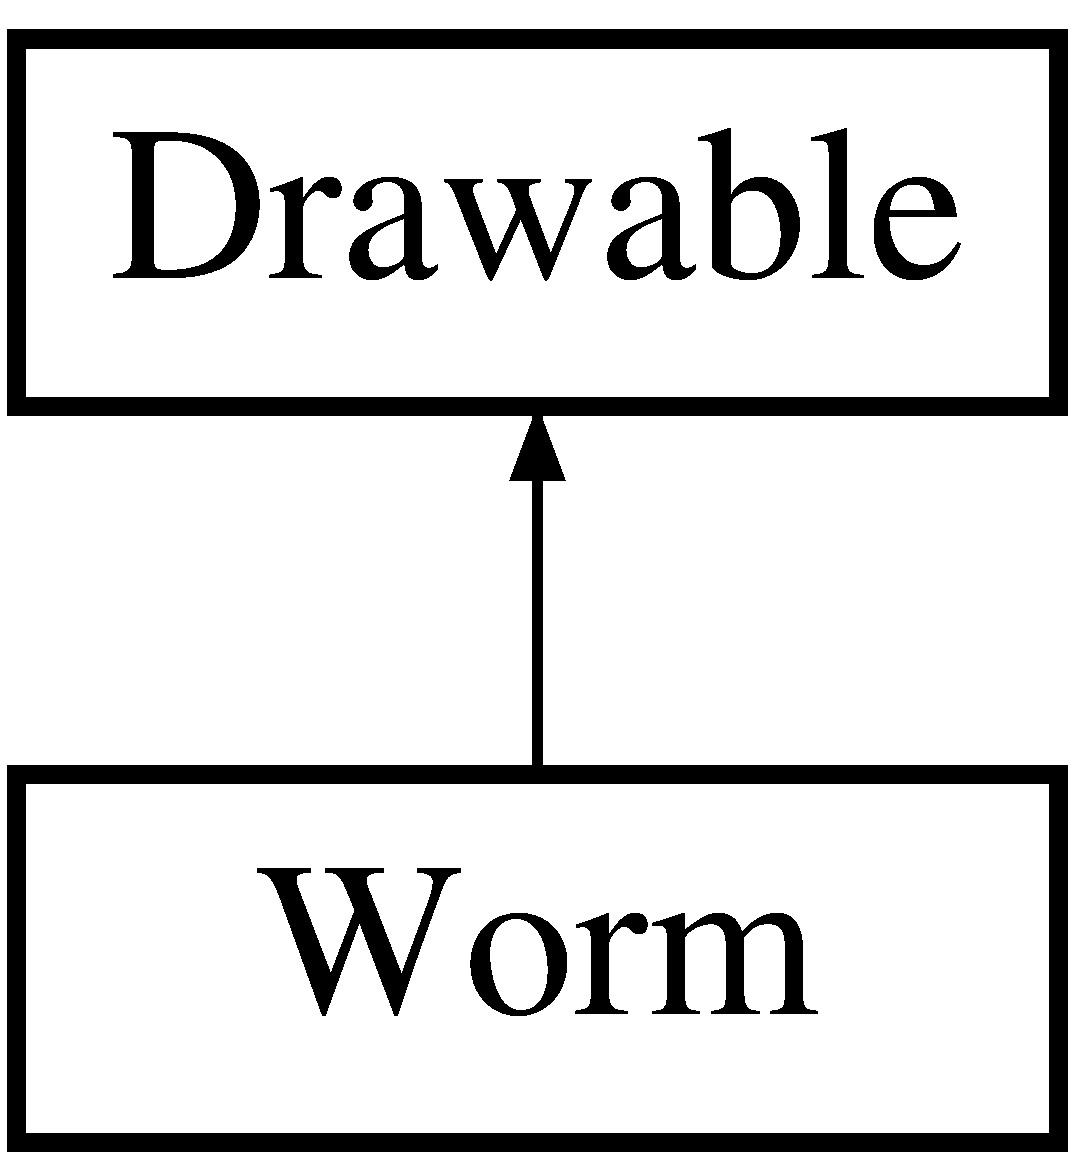
\includegraphics[height=2.000000cm]{class_worm}
\end{center}
\end{figure}
\subsection*{Metody publiczne}
\begin{DoxyCompactItemize}
\item 
\mbox{\hyperlink{class_worm_aaec23e2156f969303d6bfac36cae63e3}{Worm}} ()
\item 
virtual \mbox{\hyperlink{class_worm_ade7672966c551bb91663ed03e06f297f}{$\sim$\+Worm}} ()
\item 
void \mbox{\hyperlink{class_worm_adcb6219ae98887e491327c4ef02cf4b9}{update}} ()
\item 
float \mbox{\hyperlink{class_worm_ab517b492de0e583254c288cc583cbeb1}{left}} () const
\item 
float \mbox{\hyperlink{class_worm_a52905b36980b4aa37fe1b004df9edc0e}{right}} () const
\item 
float \mbox{\hyperlink{class_worm_a3d65c40350e8e0317bd594a3cb7c8bba}{top}} () const
\item 
float \mbox{\hyperlink{class_worm_a68061fb5be175ab42739a7c157d7073d}{bottom}} () const
\item 
float \mbox{\hyperlink{class_worm_a9787181c41ca3a4ac5098277e8a4a142}{get\+WormX}} () const
\item 
float \mbox{\hyperlink{class_worm_aa1a5e5334f8d3e339f15b36a9af31f27}{get\+WormY}} () const
\item 
void \mbox{\hyperlink{class_worm_a1cdb0c544127417ba4b95fd8e5d3f9fc}{stop\+Move}} ()
\item 
void \mbox{\hyperlink{class_worm_ae2d842c005b7bc4b20ae8333ebc9c19c}{move\+Up}} ()
\item 
void \mbox{\hyperlink{class_worm_a08f64ed1ed9149084d8d64296253c4be}{move\+Down}} ()
\item 
void \mbox{\hyperlink{class_worm_a93d02457a10bbbfc1d2028168419ecb8}{move\+Left}} ()
\item 
void \mbox{\hyperlink{class_worm_a6d4b33910c18b0e266e310d9b5512d75}{move\+Right}} ()
\item 
void \mbox{\hyperlink{class_worm_ae4cd763e0edd18cecab42b39142cea14}{jump}} ()
\item 
void \mbox{\hyperlink{class_worm_aa57fe22ce4031e5332d16d709e7274c8}{damage}} (float dmg)
\item 
bool \mbox{\hyperlink{class_worm_a606868b7856598eef50b8ebcd2374927}{is\+Alive}} ()
\item 
bool \mbox{\hyperlink{class_worm_a61589ff1104deb3cbf1cb6978e7f95f4}{check\+Collision}} (sf\+::\+Vector2f point)
\item 
int \mbox{\hyperlink{class_worm_a5a9fb6f1859a7b5cf6c447ea3ae0c1e5}{get\+OffsetY}} (sf\+::\+Vector2f point)
\item 
float \mbox{\hyperlink{class_worm_a72cf5070503bcba6423773de3367cdfd}{get\+Scale}} () const
\item 
sf\+::\+Sprite \mbox{\hyperlink{class_worm_a9b314b9a4bb91830aac7f616ef071c07}{get\+Sprite}} () const
\item 
void \mbox{\hyperlink{class_worm_a9f2a337a176e5186c7227880337c98c3}{set\+Weapon}} (\mbox{\hyperlink{class_weapon}{Weapon}} $\ast$weapon)
\item 
\mbox{\hyperlink{class_weapon}{Weapon}} $\ast$ \mbox{\hyperlink{class_worm_a42f56e4d14502d65c500fb20bd31a561}{get\+Weapon}} () const
\item 
void \mbox{\hyperlink{class_worm_adbede9b2b03f764f71629a299aec5299}{delete\+Weapon}} ()
\item 
void \mbox{\hyperlink{class_worm_af851e558c46b33b245b96a43bb2e5c56}{set\+Col\+Map}} (sf\+::\+Image $\ast$image)
\item 
sf\+::\+Text \mbox{\hyperlink{class_worm_afed2a8beb878659d49977440293ef884}{get\+Debug\+Txt}} ()
\item 
bool \mbox{\hyperlink{class_worm_a3a90a91ddbe99e67f48e54a57d12b5c7}{is\+Looking\+On\+Left}} () const
\item 
bool \mbox{\hyperlink{class_worm_a15fc66d733ecfe886495910f591d1a34}{has\+Weapon}} () const
\item 
void \mbox{\hyperlink{class_worm_a8eb6b3e55c2e6cb7c87b1593f34dac52}{set\+Team}} (\mbox{\hyperlink{_worm_8h_ae79581ee1998185d7cb41ab84352b97e}{team}} t)
\item 
void \mbox{\hyperlink{class_worm_a84fbbdac67be083a5492bf38cf83544b}{look\+Left}} ()
\item 
void \mbox{\hyperlink{class_worm_a4dbc714c26c5b09a94bd53f10172b4c1}{look\+Right}} ()
\item 
void \mbox{\hyperlink{class_worm_ac5daf6e0926f483415886c5ae297714a}{set\+Choosen}} ()
\item 
void \mbox{\hyperlink{class_worm_ab316cd13ecdfe9696e28687bfce47a4c}{set\+Normal}} ()
\end{DoxyCompactItemize}
\subsection*{Atrybuty publiczne}
\begin{DoxyCompactItemize}
\item 
sf\+::\+Vector2f \mbox{\hyperlink{class_worm_a6e519d20cdeca0c88847c0b7284ca302}{collision\+Points}} \mbox{[}8\mbox{]}
\end{DoxyCompactItemize}
\subsection*{Metody chronione}
\begin{DoxyCompactItemize}
\item 
void \mbox{\hyperlink{class_worm_adc9fd6dc3b770d4feada327666f31ee3}{draw}} (sf\+::\+Render\+Target \&target, sf\+::\+Render\+States states) const override
\end{DoxyCompactItemize}


\subsection{Opis szczegółowy}


Definicja w linii 9 pliku Worm.\+h.



\subsection{Dokumentacja konstruktora i destruktora}
\mbox{\Hypertarget{class_worm_aaec23e2156f969303d6bfac36cae63e3}\label{class_worm_aaec23e2156f969303d6bfac36cae63e3}} 
\index{Worm@{Worm}!Worm@{Worm}}
\index{Worm@{Worm}!Worm@{Worm}}
\subsubsection{\texorpdfstring{Worm()}{Worm()}}
{\footnotesize\ttfamily Worm\+::\+Worm (\begin{DoxyParamCaption}{ }\end{DoxyParamCaption})}



Definicja w linii 8 pliku Worm.\+cpp.

\mbox{\Hypertarget{class_worm_ade7672966c551bb91663ed03e06f297f}\label{class_worm_ade7672966c551bb91663ed03e06f297f}} 
\index{Worm@{Worm}!````~Worm@{$\sim$\+Worm}}
\index{````~Worm@{$\sim$\+Worm}!Worm@{Worm}}
\subsubsection{\texorpdfstring{$\sim$\+Worm()}{~Worm()}}
{\footnotesize\ttfamily Worm\+::$\sim$\+Worm (\begin{DoxyParamCaption}{ }\end{DoxyParamCaption})\hspace{0.3cm}{\ttfamily [virtual]}}



Definicja w linii 65 pliku Worm.\+cpp.



\subsection{Dokumentacja funkcji składowych}
\mbox{\Hypertarget{class_worm_a68061fb5be175ab42739a7c157d7073d}\label{class_worm_a68061fb5be175ab42739a7c157d7073d}} 
\index{Worm@{Worm}!bottom@{bottom}}
\index{bottom@{bottom}!Worm@{Worm}}
\subsubsection{\texorpdfstring{bottom()}{bottom()}}
{\footnotesize\ttfamily float Worm\+::bottom (\begin{DoxyParamCaption}{ }\end{DoxyParamCaption}) const}



Definicja w linii 239 pliku Worm.\+cpp.

\mbox{\Hypertarget{class_worm_a61589ff1104deb3cbf1cb6978e7f95f4}\label{class_worm_a61589ff1104deb3cbf1cb6978e7f95f4}} 
\index{Worm@{Worm}!check\+Collision@{check\+Collision}}
\index{check\+Collision@{check\+Collision}!Worm@{Worm}}
\subsubsection{\texorpdfstring{check\+Collision()}{checkCollision()}}
{\footnotesize\ttfamily bool Worm\+::check\+Collision (\begin{DoxyParamCaption}\item[{sf\+::\+Vector2f}]{point }\end{DoxyParamCaption})}



Definicja w linii 197 pliku Worm.\+cpp.

\mbox{\Hypertarget{class_worm_aa57fe22ce4031e5332d16d709e7274c8}\label{class_worm_aa57fe22ce4031e5332d16d709e7274c8}} 
\index{Worm@{Worm}!damage@{damage}}
\index{damage@{damage}!Worm@{Worm}}
\subsubsection{\texorpdfstring{damage()}{damage()}}
{\footnotesize\ttfamily void Worm\+::damage (\begin{DoxyParamCaption}\item[{float}]{dmg }\end{DoxyParamCaption})}



Definicja w linii 365 pliku Worm.\+cpp.

\mbox{\Hypertarget{class_worm_adbede9b2b03f764f71629a299aec5299}\label{class_worm_adbede9b2b03f764f71629a299aec5299}} 
\index{Worm@{Worm}!delete\+Weapon@{delete\+Weapon}}
\index{delete\+Weapon@{delete\+Weapon}!Worm@{Worm}}
\subsubsection{\texorpdfstring{delete\+Weapon()}{deleteWeapon()}}
{\footnotesize\ttfamily void Worm\+::delete\+Weapon (\begin{DoxyParamCaption}{ }\end{DoxyParamCaption})}



Definicja w linii 191 pliku Worm.\+cpp.

\mbox{\Hypertarget{class_worm_adc9fd6dc3b770d4feada327666f31ee3}\label{class_worm_adc9fd6dc3b770d4feada327666f31ee3}} 
\index{Worm@{Worm}!draw@{draw}}
\index{draw@{draw}!Worm@{Worm}}
\subsubsection{\texorpdfstring{draw()}{draw()}}
{\footnotesize\ttfamily void Worm\+::draw (\begin{DoxyParamCaption}\item[{sf\+::\+Render\+Target \&}]{target,  }\item[{sf\+::\+Render\+States}]{states }\end{DoxyParamCaption}) const\hspace{0.3cm}{\ttfamily [override]}, {\ttfamily [protected]}}



Definicja w linii 211 pliku Worm.\+cpp.

\mbox{\Hypertarget{class_worm_afed2a8beb878659d49977440293ef884}\label{class_worm_afed2a8beb878659d49977440293ef884}} 
\index{Worm@{Worm}!get\+Debug\+Txt@{get\+Debug\+Txt}}
\index{get\+Debug\+Txt@{get\+Debug\+Txt}!Worm@{Worm}}
\subsubsection{\texorpdfstring{get\+Debug\+Txt()}{getDebugTxt()}}
{\footnotesize\ttfamily sf\+::\+Text Worm\+::get\+Debug\+Txt (\begin{DoxyParamCaption}{ }\end{DoxyParamCaption})}



Definicja w linii 375 pliku Worm.\+cpp.

\mbox{\Hypertarget{class_worm_a5a9fb6f1859a7b5cf6c447ea3ae0c1e5}\label{class_worm_a5a9fb6f1859a7b5cf6c447ea3ae0c1e5}} 
\index{Worm@{Worm}!get\+OffsetY@{get\+OffsetY}}
\index{get\+OffsetY@{get\+OffsetY}!Worm@{Worm}}
\subsubsection{\texorpdfstring{get\+Offset\+Y()}{getOffsetY()}}
{\footnotesize\ttfamily int Worm\+::get\+OffsetY (\begin{DoxyParamCaption}\item[{sf\+::\+Vector2f}]{point }\end{DoxyParamCaption})}



Definicja w linii 153 pliku Worm.\+cpp.

\mbox{\Hypertarget{class_worm_a72cf5070503bcba6423773de3367cdfd}\label{class_worm_a72cf5070503bcba6423773de3367cdfd}} 
\index{Worm@{Worm}!get\+Scale@{get\+Scale}}
\index{get\+Scale@{get\+Scale}!Worm@{Worm}}
\subsubsection{\texorpdfstring{get\+Scale()}{getScale()}}
{\footnotesize\ttfamily float Worm\+::get\+Scale (\begin{DoxyParamCaption}{ }\end{DoxyParamCaption}) const}



Definicja w linii 168 pliku Worm.\+cpp.

\mbox{\Hypertarget{class_worm_a9b314b9a4bb91830aac7f616ef071c07}\label{class_worm_a9b314b9a4bb91830aac7f616ef071c07}} 
\index{Worm@{Worm}!get\+Sprite@{get\+Sprite}}
\index{get\+Sprite@{get\+Sprite}!Worm@{Worm}}
\subsubsection{\texorpdfstring{get\+Sprite()}{getSprite()}}
{\footnotesize\ttfamily sf\+::\+Sprite Worm\+::get\+Sprite (\begin{DoxyParamCaption}{ }\end{DoxyParamCaption}) const}



Definicja w linii 173 pliku Worm.\+cpp.

\mbox{\Hypertarget{class_worm_a42f56e4d14502d65c500fb20bd31a561}\label{class_worm_a42f56e4d14502d65c500fb20bd31a561}} 
\index{Worm@{Worm}!get\+Weapon@{get\+Weapon}}
\index{get\+Weapon@{get\+Weapon}!Worm@{Worm}}
\subsubsection{\texorpdfstring{get\+Weapon()}{getWeapon()}}
{\footnotesize\ttfamily \mbox{\hyperlink{class_weapon}{Weapon}} $\ast$ Worm\+::get\+Weapon (\begin{DoxyParamCaption}{ }\end{DoxyParamCaption}) const}



Definicja w linii 186 pliku Worm.\+cpp.

\mbox{\Hypertarget{class_worm_a9787181c41ca3a4ac5098277e8a4a142}\label{class_worm_a9787181c41ca3a4ac5098277e8a4a142}} 
\index{Worm@{Worm}!get\+WormX@{get\+WormX}}
\index{get\+WormX@{get\+WormX}!Worm@{Worm}}
\subsubsection{\texorpdfstring{get\+Worm\+X()}{getWormX()}}
{\footnotesize\ttfamily float Worm\+::get\+WormX (\begin{DoxyParamCaption}{ }\end{DoxyParamCaption}) const}



Definicja w linii 244 pliku Worm.\+cpp.

\mbox{\Hypertarget{class_worm_aa1a5e5334f8d3e339f15b36a9af31f27}\label{class_worm_aa1a5e5334f8d3e339f15b36a9af31f27}} 
\index{Worm@{Worm}!get\+WormY@{get\+WormY}}
\index{get\+WormY@{get\+WormY}!Worm@{Worm}}
\subsubsection{\texorpdfstring{get\+Worm\+Y()}{getWormY()}}
{\footnotesize\ttfamily float Worm\+::get\+WormY (\begin{DoxyParamCaption}{ }\end{DoxyParamCaption}) const}



Definicja w linii 249 pliku Worm.\+cpp.

\mbox{\Hypertarget{class_worm_a15fc66d733ecfe886495910f591d1a34}\label{class_worm_a15fc66d733ecfe886495910f591d1a34}} 
\index{Worm@{Worm}!has\+Weapon@{has\+Weapon}}
\index{has\+Weapon@{has\+Weapon}!Worm@{Worm}}
\subsubsection{\texorpdfstring{has\+Weapon()}{hasWeapon()}}
{\footnotesize\ttfamily bool Worm\+::has\+Weapon (\begin{DoxyParamCaption}{ }\end{DoxyParamCaption}) const}



Definicja w linii 395 pliku Worm.\+cpp.

\mbox{\Hypertarget{class_worm_a606868b7856598eef50b8ebcd2374927}\label{class_worm_a606868b7856598eef50b8ebcd2374927}} 
\index{Worm@{Worm}!is\+Alive@{is\+Alive}}
\index{is\+Alive@{is\+Alive}!Worm@{Worm}}
\subsubsection{\texorpdfstring{is\+Alive()}{isAlive()}}
{\footnotesize\ttfamily bool Worm\+::is\+Alive (\begin{DoxyParamCaption}{ }\end{DoxyParamCaption})}



Definicja w linii 370 pliku Worm.\+cpp.

\mbox{\Hypertarget{class_worm_a3a90a91ddbe99e67f48e54a57d12b5c7}\label{class_worm_a3a90a91ddbe99e67f48e54a57d12b5c7}} 
\index{Worm@{Worm}!is\+Looking\+On\+Left@{is\+Looking\+On\+Left}}
\index{is\+Looking\+On\+Left@{is\+Looking\+On\+Left}!Worm@{Worm}}
\subsubsection{\texorpdfstring{is\+Looking\+On\+Left()}{isLookingOnLeft()}}
{\footnotesize\ttfamily bool Worm\+::is\+Looking\+On\+Left (\begin{DoxyParamCaption}{ }\end{DoxyParamCaption}) const}



Definicja w linii 390 pliku Worm.\+cpp.

\mbox{\Hypertarget{class_worm_ae4cd763e0edd18cecab42b39142cea14}\label{class_worm_ae4cd763e0edd18cecab42b39142cea14}} 
\index{Worm@{Worm}!jump@{jump}}
\index{jump@{jump}!Worm@{Worm}}
\subsubsection{\texorpdfstring{jump()}{jump()}}
{\footnotesize\ttfamily void Worm\+::jump (\begin{DoxyParamCaption}{ }\end{DoxyParamCaption})}



Definicja w linii 354 pliku Worm.\+cpp.

\mbox{\Hypertarget{class_worm_ab517b492de0e583254c288cc583cbeb1}\label{class_worm_ab517b492de0e583254c288cc583cbeb1}} 
\index{Worm@{Worm}!left@{left}}
\index{left@{left}!Worm@{Worm}}
\subsubsection{\texorpdfstring{left()}{left()}}
{\footnotesize\ttfamily float Worm\+::left (\begin{DoxyParamCaption}{ }\end{DoxyParamCaption}) const}



Definicja w linii 227 pliku Worm.\+cpp.

\mbox{\Hypertarget{class_worm_a84fbbdac67be083a5492bf38cf83544b}\label{class_worm_a84fbbdac67be083a5492bf38cf83544b}} 
\index{Worm@{Worm}!look\+Left@{look\+Left}}
\index{look\+Left@{look\+Left}!Worm@{Worm}}
\subsubsection{\texorpdfstring{look\+Left()}{lookLeft()}}
{\footnotesize\ttfamily void Worm\+::look\+Left (\begin{DoxyParamCaption}{ }\end{DoxyParamCaption})}



Definicja w linii 280 pliku Worm.\+cpp.

\mbox{\Hypertarget{class_worm_a4dbc714c26c5b09a94bd53f10172b4c1}\label{class_worm_a4dbc714c26c5b09a94bd53f10172b4c1}} 
\index{Worm@{Worm}!look\+Right@{look\+Right}}
\index{look\+Right@{look\+Right}!Worm@{Worm}}
\subsubsection{\texorpdfstring{look\+Right()}{lookRight()}}
{\footnotesize\ttfamily void Worm\+::look\+Right (\begin{DoxyParamCaption}{ }\end{DoxyParamCaption})}



Definicja w linii 293 pliku Worm.\+cpp.

\mbox{\Hypertarget{class_worm_a08f64ed1ed9149084d8d64296253c4be}\label{class_worm_a08f64ed1ed9149084d8d64296253c4be}} 
\index{Worm@{Worm}!move\+Down@{move\+Down}}
\index{move\+Down@{move\+Down}!Worm@{Worm}}
\subsubsection{\texorpdfstring{move\+Down()}{moveDown()}}
{\footnotesize\ttfamily void Worm\+::move\+Down (\begin{DoxyParamCaption}{ }\end{DoxyParamCaption})}



Definicja w linii 272 pliku Worm.\+cpp.

\mbox{\Hypertarget{class_worm_a93d02457a10bbbfc1d2028168419ecb8}\label{class_worm_a93d02457a10bbbfc1d2028168419ecb8}} 
\index{Worm@{Worm}!move\+Left@{move\+Left}}
\index{move\+Left@{move\+Left}!Worm@{Worm}}
\subsubsection{\texorpdfstring{move\+Left()}{moveLeft()}}
{\footnotesize\ttfamily void Worm\+::move\+Left (\begin{DoxyParamCaption}{ }\end{DoxyParamCaption})}



Definicja w linii 318 pliku Worm.\+cpp.

\mbox{\Hypertarget{class_worm_a6d4b33910c18b0e266e310d9b5512d75}\label{class_worm_a6d4b33910c18b0e266e310d9b5512d75}} 
\index{Worm@{Worm}!move\+Right@{move\+Right}}
\index{move\+Right@{move\+Right}!Worm@{Worm}}
\subsubsection{\texorpdfstring{move\+Right()}{moveRight()}}
{\footnotesize\ttfamily void Worm\+::move\+Right (\begin{DoxyParamCaption}{ }\end{DoxyParamCaption})}



Definicja w linii 336 pliku Worm.\+cpp.

\mbox{\Hypertarget{class_worm_ae2d842c005b7bc4b20ae8333ebc9c19c}\label{class_worm_ae2d842c005b7bc4b20ae8333ebc9c19c}} 
\index{Worm@{Worm}!move\+Up@{move\+Up}}
\index{move\+Up@{move\+Up}!Worm@{Worm}}
\subsubsection{\texorpdfstring{move\+Up()}{moveUp()}}
{\footnotesize\ttfamily void Worm\+::move\+Up (\begin{DoxyParamCaption}{ }\end{DoxyParamCaption})}



Definicja w linii 265 pliku Worm.\+cpp.

\mbox{\Hypertarget{class_worm_a52905b36980b4aa37fe1b004df9edc0e}\label{class_worm_a52905b36980b4aa37fe1b004df9edc0e}} 
\index{Worm@{Worm}!right@{right}}
\index{right@{right}!Worm@{Worm}}
\subsubsection{\texorpdfstring{right()}{right()}}
{\footnotesize\ttfamily float Worm\+::right (\begin{DoxyParamCaption}{ }\end{DoxyParamCaption}) const}



Definicja w linii 231 pliku Worm.\+cpp.

\mbox{\Hypertarget{class_worm_ac5daf6e0926f483415886c5ae297714a}\label{class_worm_ac5daf6e0926f483415886c5ae297714a}} 
\index{Worm@{Worm}!set\+Choosen@{set\+Choosen}}
\index{set\+Choosen@{set\+Choosen}!Worm@{Worm}}
\subsubsection{\texorpdfstring{set\+Choosen()}{setChoosen()}}
{\footnotesize\ttfamily void Worm\+::set\+Choosen (\begin{DoxyParamCaption}{ }\end{DoxyParamCaption})}



Definicja w linii 307 pliku Worm.\+cpp.

\mbox{\Hypertarget{class_worm_af851e558c46b33b245b96a43bb2e5c56}\label{class_worm_af851e558c46b33b245b96a43bb2e5c56}} 
\index{Worm@{Worm}!set\+Col\+Map@{set\+Col\+Map}}
\index{set\+Col\+Map@{set\+Col\+Map}!Worm@{Worm}}
\subsubsection{\texorpdfstring{set\+Col\+Map()}{setColMap()}}
{\footnotesize\ttfamily void Worm\+::set\+Col\+Map (\begin{DoxyParamCaption}\item[{sf\+::\+Image $\ast$}]{image }\end{DoxyParamCaption})}



Definicja w linii 149 pliku Worm.\+cpp.

\mbox{\Hypertarget{class_worm_ab316cd13ecdfe9696e28687bfce47a4c}\label{class_worm_ab316cd13ecdfe9696e28687bfce47a4c}} 
\index{Worm@{Worm}!set\+Normal@{set\+Normal}}
\index{set\+Normal@{set\+Normal}!Worm@{Worm}}
\subsubsection{\texorpdfstring{set\+Normal()}{setNormal()}}
{\footnotesize\ttfamily void Worm\+::set\+Normal (\begin{DoxyParamCaption}{ }\end{DoxyParamCaption})}



Definicja w linii 313 pliku Worm.\+cpp.

\mbox{\Hypertarget{class_worm_a8eb6b3e55c2e6cb7c87b1593f34dac52}\label{class_worm_a8eb6b3e55c2e6cb7c87b1593f34dac52}} 
\index{Worm@{Worm}!set\+Team@{set\+Team}}
\index{set\+Team@{set\+Team}!Worm@{Worm}}
\subsubsection{\texorpdfstring{set\+Team()}{setTeam()}}
{\footnotesize\ttfamily void Worm\+::set\+Team (\begin{DoxyParamCaption}\item[{\mbox{\hyperlink{_worm_8h_ae79581ee1998185d7cb41ab84352b97e}{team}}}]{t }\end{DoxyParamCaption})}



Definicja w linii 400 pliku Worm.\+cpp.

\mbox{\Hypertarget{class_worm_a9f2a337a176e5186c7227880337c98c3}\label{class_worm_a9f2a337a176e5186c7227880337c98c3}} 
\index{Worm@{Worm}!set\+Weapon@{set\+Weapon}}
\index{set\+Weapon@{set\+Weapon}!Worm@{Worm}}
\subsubsection{\texorpdfstring{set\+Weapon()}{setWeapon()}}
{\footnotesize\ttfamily void Worm\+::set\+Weapon (\begin{DoxyParamCaption}\item[{\mbox{\hyperlink{class_weapon}{Weapon}} $\ast$}]{weapon }\end{DoxyParamCaption})}



Definicja w linii 178 pliku Worm.\+cpp.

\mbox{\Hypertarget{class_worm_a1cdb0c544127417ba4b95fd8e5d3f9fc}\label{class_worm_a1cdb0c544127417ba4b95fd8e5d3f9fc}} 
\index{Worm@{Worm}!stop\+Move@{stop\+Move}}
\index{stop\+Move@{stop\+Move}!Worm@{Worm}}
\subsubsection{\texorpdfstring{stop\+Move()}{stopMove()}}
{\footnotesize\ttfamily void Worm\+::stop\+Move (\begin{DoxyParamCaption}{ }\end{DoxyParamCaption})}



Definicja w linii 254 pliku Worm.\+cpp.

\mbox{\Hypertarget{class_worm_a3d65c40350e8e0317bd594a3cb7c8bba}\label{class_worm_a3d65c40350e8e0317bd594a3cb7c8bba}} 
\index{Worm@{Worm}!top@{top}}
\index{top@{top}!Worm@{Worm}}
\subsubsection{\texorpdfstring{top()}{top()}}
{\footnotesize\ttfamily float Worm\+::top (\begin{DoxyParamCaption}{ }\end{DoxyParamCaption}) const}



Definicja w linii 235 pliku Worm.\+cpp.

\mbox{\Hypertarget{class_worm_adcb6219ae98887e491327c4ef02cf4b9}\label{class_worm_adcb6219ae98887e491327c4ef02cf4b9}} 
\index{Worm@{Worm}!update@{update}}
\index{update@{update}!Worm@{Worm}}
\subsubsection{\texorpdfstring{update()}{update()}}
{\footnotesize\ttfamily void Worm\+::update (\begin{DoxyParamCaption}{ }\end{DoxyParamCaption})}



Definicja w linii 70 pliku Worm.\+cpp.



\subsection{Dokumentacja atrybutów składowych}
\mbox{\Hypertarget{class_worm_a6e519d20cdeca0c88847c0b7284ca302}\label{class_worm_a6e519d20cdeca0c88847c0b7284ca302}} 
\index{Worm@{Worm}!collision\+Points@{collision\+Points}}
\index{collision\+Points@{collision\+Points}!Worm@{Worm}}
\subsubsection{\texorpdfstring{collision\+Points}{collisionPoints}}
{\footnotesize\ttfamily sf\+::\+Vector2f Worm\+::collision\+Points\mbox{[}8\mbox{]}}



Definicja w linii 33 pliku Worm.\+h.



Dokumentacja dla tej klasy została wygenerowana z plików\+:\begin{DoxyCompactItemize}
\item 
D\+:/\+Projekty/\+C++/\+Programowanie w C2/\+Worms 2\+D/\+Worms 2\+D/\mbox{\hyperlink{_worm_8h}{Worm.\+h}}\item 
D\+:/\+Projekty/\+C++/\+Programowanie w C2/\+Worms 2\+D/\+Worms 2\+D/\mbox{\hyperlink{_worm_8cpp}{Worm.\+cpp}}\end{DoxyCompactItemize}

\chapter{Dokumentacja plików}
\hypertarget{_bazooka_8cpp}{}\section{Dokumentacja pliku D\+:/\+Projekty/\+C++/\+Programowanie w C2/\+Worms 2\+D/\+Worms 2\+D/\+Bazooka.cpp}
\label{_bazooka_8cpp}\index{D\+:/\+Projekty/\+C++/\+Programowanie w C2/\+Worms 2\+D/\+Worms 2\+D/\+Bazooka.\+cpp@{D\+:/\+Projekty/\+C++/\+Programowanie w C2/\+Worms 2\+D/\+Worms 2\+D/\+Bazooka.\+cpp}}
{\ttfamily \#include \char`\"{}Bazooka.\+h\char`\"{}}\newline
{\ttfamily \#include \char`\"{}Game\+Window.\+h\char`\"{}}\newline

\hypertarget{_bazooka_8h}{}\section{Dokumentacja pliku D\+:/\+Projekty/\+C++/\+Programowanie w C2/\+Worms 2\+D/\+Worms 2\+D/\+Bazooka.h}
\label{_bazooka_8h}\index{D\+:/\+Projekty/\+C++/\+Programowanie w C2/\+Worms 2\+D/\+Worms 2\+D/\+Bazooka.\+h@{D\+:/\+Projekty/\+C++/\+Programowanie w C2/\+Worms 2\+D/\+Worms 2\+D/\+Bazooka.\+h}}
{\ttfamily \#include \char`\"{}Weapon.\+h\char`\"{}}\newline
\subsection*{Komponenty}
\begin{DoxyCompactItemize}
\item 
class \mbox{\hyperlink{class_bazooka}{Bazooka}}
\end{DoxyCompactItemize}

\hypertarget{_bullet_8cpp}{}\section{Dokumentacja pliku D\+:/\+Projekty/\+C++/\+Programowanie w C2/\+Worms 2\+D/\+Worms 2\+D/\+Bullet.cpp}
\label{_bullet_8cpp}\index{D\+:/\+Projekty/\+C++/\+Programowanie w C2/\+Worms 2\+D/\+Worms 2\+D/\+Bullet.\+cpp@{D\+:/\+Projekty/\+C++/\+Programowanie w C2/\+Worms 2\+D/\+Worms 2\+D/\+Bullet.\+cpp}}
{\ttfamily \#include \char`\"{}Bullet.\+h\char`\"{}}\newline

\hypertarget{_bullet_8h}{}\section{Dokumentacja pliku D\+:/\+Projekty/\+C++/\+Programowanie w C2/\+Worms 2\+D/\+Worms 2\+D/\+Bullet.h}
\label{_bullet_8h}\index{D\+:/\+Projekty/\+C++/\+Programowanie w C2/\+Worms 2\+D/\+Worms 2\+D/\+Bullet.\+h@{D\+:/\+Projekty/\+C++/\+Programowanie w C2/\+Worms 2\+D/\+Worms 2\+D/\+Bullet.\+h}}
{\ttfamily \#include $<$S\+F\+M\+L/\+Graphics/\+Drawable.\+hpp$>$}\newline
{\ttfamily \#include $<$S\+F\+M\+L/\+Graphics/\+Sprite.\+hpp$>$}\newline
{\ttfamily \#include $<$S\+F\+M\+L/\+Graphics/\+Texture.\+hpp$>$}\newline
{\ttfamily \#include $<$S\+F\+M\+L/\+Graphics/\+Render\+Target.\+hpp$>$}\newline
\subsection*{Komponenty}
\begin{DoxyCompactItemize}
\item 
class \mbox{\hyperlink{class_bullet}{Bullet}}
\end{DoxyCompactItemize}

\hypertarget{_button_8cpp}{}\section{Dokumentacja pliku D\+:/\+Projekty/\+C++/\+Programowanie w C2/\+Worms 2\+D/\+Worms 2\+D/\+Button.cpp}
\label{_button_8cpp}\index{D\+:/\+Projekty/\+C++/\+Programowanie w C2/\+Worms 2\+D/\+Worms 2\+D/\+Button.\+cpp@{D\+:/\+Projekty/\+C++/\+Programowanie w C2/\+Worms 2\+D/\+Worms 2\+D/\+Button.\+cpp}}
{\ttfamily \#include \char`\"{}Button.\+h\char`\"{}}\newline

\hypertarget{_button_8h}{}\section{Dokumentacja pliku D\+:/\+Projekty/\+C++/\+Programowanie w C2/\+Worms 2\+D/\+Worms 2\+D/\+Button.h}
\label{_button_8h}\index{D\+:/\+Projekty/\+C++/\+Programowanie w C2/\+Worms 2\+D/\+Worms 2\+D/\+Button.\+h@{D\+:/\+Projekty/\+C++/\+Programowanie w C2/\+Worms 2\+D/\+Worms 2\+D/\+Button.\+h}}
{\ttfamily \#include $<$S\+F\+M\+L/\+Graphics.\+hpp$>$}\newline
\subsection*{Komponenty}
\begin{DoxyCompactItemize}
\item 
class \mbox{\hyperlink{class_button}{Button}}
\begin{DoxyCompactList}\small\item\em Klasa przycisku. \end{DoxyCompactList}\end{DoxyCompactItemize}

\hypertarget{_f_p_s_counter_8cpp}{}\section{Dokumentacja pliku D\+:/\+Projekty/\+C++/\+Programowanie w C2/\+Worms 2\+D/\+Worms 2\+D/\+F\+P\+S\+Counter.cpp}
\label{_f_p_s_counter_8cpp}\index{D\+:/\+Projekty/\+C++/\+Programowanie w C2/\+Worms 2\+D/\+Worms 2\+D/\+F\+P\+S\+Counter.\+cpp@{D\+:/\+Projekty/\+C++/\+Programowanie w C2/\+Worms 2\+D/\+Worms 2\+D/\+F\+P\+S\+Counter.\+cpp}}
{\ttfamily \#include \char`\"{}F\+P\+S\+Counter.\+h\char`\"{}}\newline
{\ttfamily \#include $<$iostream$>$}\newline
{\ttfamily \#include \char`\"{}Game\+Window.\+h\char`\"{}}\newline

\hypertarget{_f_p_s_counter_8h}{}\section{Dokumentacja pliku D\+:/\+Projekty/\+C++/\+Programowanie w C2/\+Worms 2\+D/\+Worms 2\+D/\+F\+P\+S\+Counter.h}
\label{_f_p_s_counter_8h}\index{D\+:/\+Projekty/\+C++/\+Programowanie w C2/\+Worms 2\+D/\+Worms 2\+D/\+F\+P\+S\+Counter.\+h@{D\+:/\+Projekty/\+C++/\+Programowanie w C2/\+Worms 2\+D/\+Worms 2\+D/\+F\+P\+S\+Counter.\+h}}
{\ttfamily \#include $<$S\+F\+M\+L/\+Graphics.\+hpp$>$}\newline
\subsection*{Komponenty}
\begin{DoxyCompactItemize}
\item 
class \mbox{\hyperlink{class_f_p_s_counter}{F\+P\+S\+Counter}}
\end{DoxyCompactItemize}

\hypertarget{_game_event_8cpp}{}\section{Dokumentacja pliku D\+:/\+Projekty/\+C++/\+Programowanie w C2/\+Worms 2\+D/\+Worms 2\+D/\+Game\+Event.cpp}
\label{_game_event_8cpp}\index{D\+:/\+Projekty/\+C++/\+Programowanie w C2/\+Worms 2\+D/\+Worms 2\+D/\+Game\+Event.\+cpp@{D\+:/\+Projekty/\+C++/\+Programowanie w C2/\+Worms 2\+D/\+Worms 2\+D/\+Game\+Event.\+cpp}}
{\ttfamily \#include \char`\"{}Game\+Event.\+h\char`\"{}}\newline
{\ttfamily \#include $<$iostream$>$}\newline
{\ttfamily \#include \char`\"{}Revolver.\+h\char`\"{}}\newline

\hypertarget{_game_event_8h}{}\section{Dokumentacja pliku D\+:/\+Projekty/\+C++/\+Programowanie w C2/\+Worms 2\+D/\+Worms 2\+D/\+Game\+Event.h}
\label{_game_event_8h}\index{D\+:/\+Projekty/\+C++/\+Programowanie w C2/\+Worms 2\+D/\+Worms 2\+D/\+Game\+Event.\+h@{D\+:/\+Projekty/\+C++/\+Programowanie w C2/\+Worms 2\+D/\+Worms 2\+D/\+Game\+Event.\+h}}
{\ttfamily \#include $<$S\+F\+M\+L/\+Graphics.\+hpp$>$}\newline
{\ttfamily \#include \char`\"{}Game\+Window.\+h\char`\"{}}\newline
{\ttfamily \#include $<$vector$>$}\newline
\subsection*{Komponenty}
\begin{DoxyCompactItemize}
\item 
class \mbox{\hyperlink{class_game_event}{Game\+Event}}
\end{DoxyCompactItemize}

\hypertarget{_game_sound_8cpp}{}\section{Dokumentacja pliku D\+:/\+Projekty/\+C++/\+Programowanie w C2/\+Worms 2\+D/\+Worms 2\+D/\+Game\+Sound.cpp}
\label{_game_sound_8cpp}\index{D\+:/\+Projekty/\+C++/\+Programowanie w C2/\+Worms 2\+D/\+Worms 2\+D/\+Game\+Sound.\+cpp@{D\+:/\+Projekty/\+C++/\+Programowanie w C2/\+Worms 2\+D/\+Worms 2\+D/\+Game\+Sound.\+cpp}}
{\ttfamily \#include \char`\"{}Game\+Sound.\+h\char`\"{}}\newline

\hypertarget{_game_sound_8h}{}\section{Dokumentacja pliku D\+:/\+Projekty/\+C++/\+Programowanie w C2/\+Worms 2\+D/\+Worms 2\+D/\+Game\+Sound.h}
\label{_game_sound_8h}\index{D\+:/\+Projekty/\+C++/\+Programowanie w C2/\+Worms 2\+D/\+Worms 2\+D/\+Game\+Sound.\+h@{D\+:/\+Projekty/\+C++/\+Programowanie w C2/\+Worms 2\+D/\+Worms 2\+D/\+Game\+Sound.\+h}}
{\ttfamily \#include $<$string$>$}\newline
{\ttfamily \#include $<$S\+F\+M\+L/\+Audio.\+hpp$>$}\newline
{\ttfamily \#include $<$iostream$>$}\newline
\subsection*{Komponenty}
\begin{DoxyCompactItemize}
\item 
class \mbox{\hyperlink{class_game_sound}{Game\+Sound}}
\begin{DoxyCompactList}\small\item\em Klasa dźwięków gry. \end{DoxyCompactList}\end{DoxyCompactItemize}

\hypertarget{_game_window_8cpp}{}\section{Dokumentacja pliku D\+:/\+Projekty/\+C++/\+Programowanie w C2/\+Worms 2\+D/\+Worms 2\+D/\+Game\+Window.cpp}
\label{_game_window_8cpp}\index{D\+:/\+Projekty/\+C++/\+Programowanie w C2/\+Worms 2\+D/\+Worms 2\+D/\+Game\+Window.\+cpp@{D\+:/\+Projekty/\+C++/\+Programowanie w C2/\+Worms 2\+D/\+Worms 2\+D/\+Game\+Window.\+cpp}}
{\ttfamily \#include \char`\"{}Game\+Window.\+h\char`\"{}}\newline
{\ttfamily \#include \char`\"{}Bullet.\+h\char`\"{}}\newline

\hypertarget{_game_window_8h}{}\section{Dokumentacja pliku D\+:/\+Projekty/\+C++/\+Programowanie w C2/\+Worms 2\+D/\+Worms 2\+D/\+Game\+Window.h}
\label{_game_window_8h}\index{D\+:/\+Projekty/\+C++/\+Programowanie w C2/\+Worms 2\+D/\+Worms 2\+D/\+Game\+Window.\+h@{D\+:/\+Projekty/\+C++/\+Programowanie w C2/\+Worms 2\+D/\+Worms 2\+D/\+Game\+Window.\+h}}
{\ttfamily \#include $<$string$>$}\newline
{\ttfamily \#include $<$S\+F\+M\+L/\+Graphics.\+hpp$>$}\newline
{\ttfamily \#include $<$vector$>$}\newline
{\ttfamily \#include \char`\"{}F\+P\+S\+Counter.\+h\char`\"{}}\newline
{\ttfamily \#include \char`\"{}Worm.\+h\char`\"{}}\newline
{\ttfamily \#include \char`\"{}Game\+Sound.\+h\char`\"{}}\newline
{\ttfamily \#include \char`\"{}Terrain.\+h\char`\"{}}\newline
{\ttfamily \#include \char`\"{}Bullet.\+h\char`\"{}}\newline
{\ttfamily \#include \char`\"{}Weapon.\+h\char`\"{}}\newline
{\ttfamily \#include \char`\"{}Bazooka.\+h\char`\"{}}\newline
{\ttfamily \#include \char`\"{}Water.\+h\char`\"{}}\newline
{\ttfamily \#include \char`\"{}Menu.\+h\char`\"{}}\newline
\subsection*{Komponenty}
\begin{DoxyCompactItemize}
\item 
class \mbox{\hyperlink{class_game_window}{Game\+Window}}
\end{DoxyCompactItemize}

\hypertarget{_menu_8cpp}{}\section{Dokumentacja pliku D\+:/\+Projekty/\+C++/\+Programowanie w C2/\+Worms 2\+D/\+Worms 2\+D/\+Menu.cpp}
\label{_menu_8cpp}\index{D\+:/\+Projekty/\+C++/\+Programowanie w C2/\+Worms 2\+D/\+Worms 2\+D/\+Menu.\+cpp@{D\+:/\+Projekty/\+C++/\+Programowanie w C2/\+Worms 2\+D/\+Worms 2\+D/\+Menu.\+cpp}}
{\ttfamily \#include \char`\"{}Menu.\+h\char`\"{}}\newline
{\ttfamily \#include $<$iostream$>$}\newline
{\ttfamily \#include \char`\"{}Game\+Sound.\+h\char`\"{}}\newline
{\ttfamily \#include \char`\"{}Game\+Window.\+h\char`\"{}}\newline

\hypertarget{_menu_8h}{}\section{Dokumentacja pliku D\+:/\+Projekty/\+C++/\+Programowanie w C2/\+Worms 2\+D/\+Worms 2\+D/\+Menu.h}
\label{_menu_8h}\index{D\+:/\+Projekty/\+C++/\+Programowanie w C2/\+Worms 2\+D/\+Worms 2\+D/\+Menu.\+h@{D\+:/\+Projekty/\+C++/\+Programowanie w C2/\+Worms 2\+D/\+Worms 2\+D/\+Menu.\+h}}
{\ttfamily \#include $<$S\+F\+M\+L/\+Graphics.\+hpp$>$}\newline
{\ttfamily \#include \char`\"{}Button.\+h\char`\"{}}\newline
{\ttfamily \#include $<$vector$>$}\newline
\subsection*{Komponenty}
\begin{DoxyCompactItemize}
\item 
class \mbox{\hyperlink{class_menu}{Menu}}
\end{DoxyCompactItemize}
\subsection*{Wyliczenia}
\begin{DoxyCompactItemize}
\item 
enum \mbox{\hyperlink{_menu_8h_ab0edca8721ed515bb9906f1c3e538c60}{game\+\_\+states}} \{ \newline
\mbox{\hyperlink{_menu_8h_ab0edca8721ed515bb9906f1c3e538c60ad50cf309d7568040619ed26ee6835a84}{G\+A\+ME}}, 
\mbox{\hyperlink{_menu_8h_ab0edca8721ed515bb9906f1c3e538c60a56b36d0d0bb01b339cf1041adc08e262}{P\+A\+U\+SE}}, 
\mbox{\hyperlink{_menu_8h_ab0edca8721ed515bb9906f1c3e538c60a4c40e60bc71a32b924ce1f08d57f9721}{M\+E\+NU}}, 
\mbox{\hyperlink{_menu_8h_ab0edca8721ed515bb9906f1c3e538c60a9f5cb747b2e1f0ea781d2b1f2a5b4824}{H\+E\+LP}}, 
\newline
\mbox{\hyperlink{_menu_8h_ab0edca8721ed515bb9906f1c3e538c60a3ac9fba6b0ae8890116f0c18730bacd7}{H\+E\+L\+P\+\_\+\+P\+A\+U\+SE}}, 
\mbox{\hyperlink{_menu_8h_ab0edca8721ed515bb9906f1c3e538c60a34fc7bcc4121e170f43e668bf806d56f}{R\+E\+D\+\_\+\+W\+IN}}, 
\mbox{\hyperlink{_menu_8h_ab0edca8721ed515bb9906f1c3e538c60afa9ff0ce517298c80a045e4acbe471c9}{B\+L\+U\+E\+\_\+\+W\+IN}}, 
\mbox{\hyperlink{_menu_8h_ab0edca8721ed515bb9906f1c3e538c60a7a10b5d68d31711288e1fe0fa17dbf4f}{E\+X\+IT}}, 
\newline
\mbox{\hyperlink{_menu_8h_ab0edca8721ed515bb9906f1c3e538c60ad14e2514427609da194a72091721f4c7}{K\+E\+Y\+B\+O\+A\+RD}}, 
\mbox{\hyperlink{_menu_8h_ab0edca8721ed515bb9906f1c3e538c60a273c15ddc1f5abadaf24cd191e7db5e0}{G\+A\+M\+E\+P\+AD}}
 \}
\end{DoxyCompactItemize}


\subsection{Dokumentacja typów wyliczanych}
\mbox{\Hypertarget{_menu_8h_ab0edca8721ed515bb9906f1c3e538c60}\label{_menu_8h_ab0edca8721ed515bb9906f1c3e538c60}} 
\index{Menu.\+h@{Menu.\+h}!game\+\_\+states@{game\+\_\+states}}
\index{game\+\_\+states@{game\+\_\+states}!Menu.\+h@{Menu.\+h}}
\subsubsection{\texorpdfstring{game\+\_\+states}{game\_states}}
{\footnotesize\ttfamily enum \mbox{\hyperlink{_menu_8h_ab0edca8721ed515bb9906f1c3e538c60}{game\+\_\+states}}}

\begin{DoxyEnumFields}{Wartości wyliczeń}
\raisebox{\heightof{T}}[0pt][0pt]{\index{G\+A\+ME@{G\+A\+ME}!Menu.\+h@{Menu.\+h}}\index{Menu.\+h@{Menu.\+h}!G\+A\+ME@{G\+A\+ME}}}\mbox{\Hypertarget{_menu_8h_ab0edca8721ed515bb9906f1c3e538c60ad50cf309d7568040619ed26ee6835a84}\label{_menu_8h_ab0edca8721ed515bb9906f1c3e538c60ad50cf309d7568040619ed26ee6835a84}} 
G\+A\+ME&\\
\hline

\raisebox{\heightof{T}}[0pt][0pt]{\index{P\+A\+U\+SE@{P\+A\+U\+SE}!Menu.\+h@{Menu.\+h}}\index{Menu.\+h@{Menu.\+h}!P\+A\+U\+SE@{P\+A\+U\+SE}}}\mbox{\Hypertarget{_menu_8h_ab0edca8721ed515bb9906f1c3e538c60a56b36d0d0bb01b339cf1041adc08e262}\label{_menu_8h_ab0edca8721ed515bb9906f1c3e538c60a56b36d0d0bb01b339cf1041adc08e262}} 
P\+A\+U\+SE&\\
\hline

\raisebox{\heightof{T}}[0pt][0pt]{\index{M\+E\+NU@{M\+E\+NU}!Menu.\+h@{Menu.\+h}}\index{Menu.\+h@{Menu.\+h}!M\+E\+NU@{M\+E\+NU}}}\mbox{\Hypertarget{_menu_8h_ab0edca8721ed515bb9906f1c3e538c60a4c40e60bc71a32b924ce1f08d57f9721}\label{_menu_8h_ab0edca8721ed515bb9906f1c3e538c60a4c40e60bc71a32b924ce1f08d57f9721}} 
M\+E\+NU&\\
\hline

\raisebox{\heightof{T}}[0pt][0pt]{\index{H\+E\+LP@{H\+E\+LP}!Menu.\+h@{Menu.\+h}}\index{Menu.\+h@{Menu.\+h}!H\+E\+LP@{H\+E\+LP}}}\mbox{\Hypertarget{_menu_8h_ab0edca8721ed515bb9906f1c3e538c60a9f5cb747b2e1f0ea781d2b1f2a5b4824}\label{_menu_8h_ab0edca8721ed515bb9906f1c3e538c60a9f5cb747b2e1f0ea781d2b1f2a5b4824}} 
H\+E\+LP&\\
\hline

\raisebox{\heightof{T}}[0pt][0pt]{\index{H\+E\+L\+P\+\_\+\+P\+A\+U\+SE@{H\+E\+L\+P\+\_\+\+P\+A\+U\+SE}!Menu.\+h@{Menu.\+h}}\index{Menu.\+h@{Menu.\+h}!H\+E\+L\+P\+\_\+\+P\+A\+U\+SE@{H\+E\+L\+P\+\_\+\+P\+A\+U\+SE}}}\mbox{\Hypertarget{_menu_8h_ab0edca8721ed515bb9906f1c3e538c60a3ac9fba6b0ae8890116f0c18730bacd7}\label{_menu_8h_ab0edca8721ed515bb9906f1c3e538c60a3ac9fba6b0ae8890116f0c18730bacd7}} 
H\+E\+L\+P\+\_\+\+P\+A\+U\+SE&\\
\hline

\raisebox{\heightof{T}}[0pt][0pt]{\index{R\+E\+D\+\_\+\+W\+IN@{R\+E\+D\+\_\+\+W\+IN}!Menu.\+h@{Menu.\+h}}\index{Menu.\+h@{Menu.\+h}!R\+E\+D\+\_\+\+W\+IN@{R\+E\+D\+\_\+\+W\+IN}}}\mbox{\Hypertarget{_menu_8h_ab0edca8721ed515bb9906f1c3e538c60a34fc7bcc4121e170f43e668bf806d56f}\label{_menu_8h_ab0edca8721ed515bb9906f1c3e538c60a34fc7bcc4121e170f43e668bf806d56f}} 
R\+E\+D\+\_\+\+W\+IN&\\
\hline

\raisebox{\heightof{T}}[0pt][0pt]{\index{B\+L\+U\+E\+\_\+\+W\+IN@{B\+L\+U\+E\+\_\+\+W\+IN}!Menu.\+h@{Menu.\+h}}\index{Menu.\+h@{Menu.\+h}!B\+L\+U\+E\+\_\+\+W\+IN@{B\+L\+U\+E\+\_\+\+W\+IN}}}\mbox{\Hypertarget{_menu_8h_ab0edca8721ed515bb9906f1c3e538c60afa9ff0ce517298c80a045e4acbe471c9}\label{_menu_8h_ab0edca8721ed515bb9906f1c3e538c60afa9ff0ce517298c80a045e4acbe471c9}} 
B\+L\+U\+E\+\_\+\+W\+IN&\\
\hline

\raisebox{\heightof{T}}[0pt][0pt]{\index{E\+X\+IT@{E\+X\+IT}!Menu.\+h@{Menu.\+h}}\index{Menu.\+h@{Menu.\+h}!E\+X\+IT@{E\+X\+IT}}}\mbox{\Hypertarget{_menu_8h_ab0edca8721ed515bb9906f1c3e538c60a7a10b5d68d31711288e1fe0fa17dbf4f}\label{_menu_8h_ab0edca8721ed515bb9906f1c3e538c60a7a10b5d68d31711288e1fe0fa17dbf4f}} 
E\+X\+IT&\\
\hline

\raisebox{\heightof{T}}[0pt][0pt]{\index{K\+E\+Y\+B\+O\+A\+RD@{K\+E\+Y\+B\+O\+A\+RD}!Menu.\+h@{Menu.\+h}}\index{Menu.\+h@{Menu.\+h}!K\+E\+Y\+B\+O\+A\+RD@{K\+E\+Y\+B\+O\+A\+RD}}}\mbox{\Hypertarget{_menu_8h_ab0edca8721ed515bb9906f1c3e538c60ad14e2514427609da194a72091721f4c7}\label{_menu_8h_ab0edca8721ed515bb9906f1c3e538c60ad14e2514427609da194a72091721f4c7}} 
K\+E\+Y\+B\+O\+A\+RD&\\
\hline

\raisebox{\heightof{T}}[0pt][0pt]{\index{G\+A\+M\+E\+P\+AD@{G\+A\+M\+E\+P\+AD}!Menu.\+h@{Menu.\+h}}\index{Menu.\+h@{Menu.\+h}!G\+A\+M\+E\+P\+AD@{G\+A\+M\+E\+P\+AD}}}\mbox{\Hypertarget{_menu_8h_ab0edca8721ed515bb9906f1c3e538c60a273c15ddc1f5abadaf24cd191e7db5e0}\label{_menu_8h_ab0edca8721ed515bb9906f1c3e538c60a273c15ddc1f5abadaf24cd191e7db5e0}} 
G\+A\+M\+E\+P\+AD&\\
\hline

\end{DoxyEnumFields}


Definicja w linii 6 pliku Menu.\+h.


\hypertarget{_revolver_8cpp}{}\section{Dokumentacja pliku D\+:/\+Projekty/\+C++/\+Programowanie w C2/\+Worms 2\+D/\+Worms 2\+D/\+Revolver.cpp}
\label{_revolver_8cpp}\index{D\+:/\+Projekty/\+C++/\+Programowanie w C2/\+Worms 2\+D/\+Worms 2\+D/\+Revolver.\+cpp@{D\+:/\+Projekty/\+C++/\+Programowanie w C2/\+Worms 2\+D/\+Worms 2\+D/\+Revolver.\+cpp}}
{\ttfamily \#include \char`\"{}Revolver.\+h\char`\"{}}\newline
{\ttfamily \#include \char`\"{}Game\+Sound.\+h\char`\"{}}\newline
{\ttfamily \#include \char`\"{}Game\+Window.\+h\char`\"{}}\newline

\hypertarget{_revolver_8h}{}\section{Dokumentacja pliku D\+:/\+Projekty/\+C++/\+Programowanie w C2/\+Worms 2\+D/\+Worms 2\+D/\+Revolver.h}
\label{_revolver_8h}\index{D\+:/\+Projekty/\+C++/\+Programowanie w C2/\+Worms 2\+D/\+Worms 2\+D/\+Revolver.\+h@{D\+:/\+Projekty/\+C++/\+Programowanie w C2/\+Worms 2\+D/\+Worms 2\+D/\+Revolver.\+h}}
{\ttfamily \#include \char`\"{}Weapon.\+h\char`\"{}}\newline
\subsection*{Komponenty}
\begin{DoxyCompactItemize}
\item 
class \mbox{\hyperlink{class_revolver}{Revolver}}
\begin{DoxyCompactList}\small\item\em Klasa rewolwera. \end{DoxyCompactList}\end{DoxyCompactItemize}

\hypertarget{_source_8cpp}{}\section{Dokumentacja pliku D\+:/\+Projekty/\+C++/\+Programowanie w C2/\+Worms 2\+D/\+Worms 2\+D/\+Source.cpp}
\label{_source_8cpp}\index{D\+:/\+Projekty/\+C++/\+Programowanie w C2/\+Worms 2\+D/\+Worms 2\+D/\+Source.\+cpp@{D\+:/\+Projekty/\+C++/\+Programowanie w C2/\+Worms 2\+D/\+Worms 2\+D/\+Source.\+cpp}}
{\ttfamily \#include \char`\"{}Game\+Event.\+h\char`\"{}}\newline
{\ttfamily \#include \char`\"{}Game\+Window.\+h\char`\"{}}\newline
{\ttfamily \#include \char`\"{}Game\+Sound.\+h\char`\"{}}\newline
\subsection*{Funkcje}
\begin{DoxyCompactItemize}
\item 
int \mbox{\hyperlink{_source_8cpp_ae66f6b31b5ad750f1fe042a706a4e3d4}{main}} ()
\end{DoxyCompactItemize}


\subsection{Dokumentacja funkcji}
\mbox{\Hypertarget{_source_8cpp_ae66f6b31b5ad750f1fe042a706a4e3d4}\label{_source_8cpp_ae66f6b31b5ad750f1fe042a706a4e3d4}} 
\index{Source.\+cpp@{Source.\+cpp}!main@{main}}
\index{main@{main}!Source.\+cpp@{Source.\+cpp}}
\subsubsection{\texorpdfstring{main()}{main()}}
{\footnotesize\ttfamily int main (\begin{DoxyParamCaption}{ }\end{DoxyParamCaption})}



Definicja w linii 6 pliku Source.\+cpp.


\hypertarget{_terrain_8cpp}{}\section{Dokumentacja pliku D\+:/\+Projekty/\+C++/\+Programowanie w C2/\+Worms 2\+D/\+Worms 2\+D/\+Terrain.cpp}
\label{_terrain_8cpp}\index{D\+:/\+Projekty/\+C++/\+Programowanie w C2/\+Worms 2\+D/\+Worms 2\+D/\+Terrain.\+cpp@{D\+:/\+Projekty/\+C++/\+Programowanie w C2/\+Worms 2\+D/\+Worms 2\+D/\+Terrain.\+cpp}}
{\ttfamily \#include \char`\"{}Terrain.\+h\char`\"{}}\newline
{\ttfamily \#include $<$iostream$>$}\newline

\hypertarget{_terrain_8h}{}\section{Dokumentacja pliku D\+:/\+Projekty/\+C++/\+Programowanie w C2/\+Worms 2\+D/\+Worms 2\+D/\+Terrain.h}
\label{_terrain_8h}\index{D\+:/\+Projekty/\+C++/\+Programowanie w C2/\+Worms 2\+D/\+Worms 2\+D/\+Terrain.\+h@{D\+:/\+Projekty/\+C++/\+Programowanie w C2/\+Worms 2\+D/\+Worms 2\+D/\+Terrain.\+h}}
{\ttfamily \#include $<$S\+F\+M\+L/\+Graphics.\+hpp$>$}\newline
\subsection*{Komponenty}
\begin{DoxyCompactItemize}
\item 
class \mbox{\hyperlink{class_terrain}{Terrain}}
\begin{DoxyCompactList}\small\item\em Klasa terenu(mapy) \end{DoxyCompactList}\end{DoxyCompactItemize}

\hypertarget{_water_8cpp}{}\section{Dokumentacja pliku D\+:/\+Projekty/\+C++/\+Programowanie w C2/\+Worms 2\+D/\+Worms 2\+D/\+Water.cpp}
\label{_water_8cpp}\index{D\+:/\+Projekty/\+C++/\+Programowanie w C2/\+Worms 2\+D/\+Worms 2\+D/\+Water.\+cpp@{D\+:/\+Projekty/\+C++/\+Programowanie w C2/\+Worms 2\+D/\+Worms 2\+D/\+Water.\+cpp}}
{\ttfamily \#include \char`\"{}Water.\+h\char`\"{}}\newline

\hypertarget{_water_8h}{}\section{Dokumentacja pliku D\+:/\+Projekty/\+C++/\+Programowanie w C2/\+Worms 2\+D/\+Worms 2\+D/\+Water.h}
\label{_water_8h}\index{D\+:/\+Projekty/\+C++/\+Programowanie w C2/\+Worms 2\+D/\+Worms 2\+D/\+Water.\+h@{D\+:/\+Projekty/\+C++/\+Programowanie w C2/\+Worms 2\+D/\+Worms 2\+D/\+Water.\+h}}
{\ttfamily \#include $<$S\+F\+M\+L/\+Graphics.\+hpp$>$}\newline
\subsection*{Komponenty}
\begin{DoxyCompactItemize}
\item 
class \mbox{\hyperlink{class_water}{Water}}
\begin{DoxyCompactList}\small\item\em Klasa wody. \end{DoxyCompactList}\end{DoxyCompactItemize}

\hypertarget{_weapon_8cpp}{}\section{Dokumentacja pliku D\+:/\+Projekty/\+C++/\+Programowanie w C2/\+Worms 2\+D/\+Worms 2\+D/\+Weapon.cpp}
\label{_weapon_8cpp}\index{D\+:/\+Projekty/\+C++/\+Programowanie w C2/\+Worms 2\+D/\+Worms 2\+D/\+Weapon.\+cpp@{D\+:/\+Projekty/\+C++/\+Programowanie w C2/\+Worms 2\+D/\+Worms 2\+D/\+Weapon.\+cpp}}
{\ttfamily \#include \char`\"{}Weapon.\+h\char`\"{}}\newline
{\ttfamily \#include $<$iostream$>$}\newline

\hypertarget{_weapon_8h}{}\section{Dokumentacja pliku D\+:/\+Projekty/\+C++/\+Programowanie w C2/\+Worms 2\+D/\+Worms 2\+D/\+Weapon.h}
\label{_weapon_8h}\index{D\+:/\+Projekty/\+C++/\+Programowanie w C2/\+Worms 2\+D/\+Worms 2\+D/\+Weapon.\+h@{D\+:/\+Projekty/\+C++/\+Programowanie w C2/\+Worms 2\+D/\+Worms 2\+D/\+Weapon.\+h}}
{\ttfamily \#include $<$S\+F\+M\+L/\+Graphics/\+Drawable.\+hpp$>$}\newline
{\ttfamily \#include $<$S\+F\+M\+L/\+Graphics/\+Sprite.\+hpp$>$}\newline
{\ttfamily \#include $<$S\+F\+M\+L/\+Graphics/\+Texture.\+hpp$>$}\newline
{\ttfamily \#include \char`\"{}Bullet.\+h\char`\"{}}\newline
\subsection*{Komponenty}
\begin{DoxyCompactItemize}
\item 
class \mbox{\hyperlink{class_weapon}{Weapon}}
\begin{DoxyCompactList}\small\item\em Klasa bazowa broni. \end{DoxyCompactList}\end{DoxyCompactItemize}

\hypertarget{_worm_8cpp}{}\section{Dokumentacja pliku D\+:/\+Projekty/\+C++/\+Programowanie w C2/\+Worms 2\+D/\+Worms 2\+D/\+Worm.cpp}
\label{_worm_8cpp}\index{D\+:/\+Projekty/\+C++/\+Programowanie w C2/\+Worms 2\+D/\+Worms 2\+D/\+Worm.\+cpp@{D\+:/\+Projekty/\+C++/\+Programowanie w C2/\+Worms 2\+D/\+Worms 2\+D/\+Worm.\+cpp}}
{\ttfamily \#include \char`\"{}Worm.\+h\char`\"{}}\newline
{\ttfamily \#include $<$string$>$}\newline
{\ttfamily \#include $<$iostream$>$}\newline
{\ttfamily \#include \char`\"{}Game\+Window.\+h\char`\"{}}\newline
{\ttfamily \#include \char`\"{}Game\+Event.\+h\char`\"{}}\newline

\hypertarget{_worm_8h}{}\section{Dokumentacja pliku D\+:/\+Projekty/\+C++/\+Programowanie w C2/\+Worms 2\+D/\+Worms 2\+D/\+Worm.h}
\label{_worm_8h}\index{D\+:/\+Projekty/\+C++/\+Programowanie w C2/\+Worms 2\+D/\+Worms 2\+D/\+Worm.\+h@{D\+:/\+Projekty/\+C++/\+Programowanie w C2/\+Worms 2\+D/\+Worms 2\+D/\+Worm.\+h}}
{\ttfamily \#include $<$S\+F\+M\+L/\+Graphics.\+hpp$>$}\newline
{\ttfamily \#include \char`\"{}Weapon.\+h\char`\"{}}\newline
\subsection*{Komponenty}
\begin{DoxyCompactItemize}
\item 
class \mbox{\hyperlink{class_worm}{Worm}}
\end{DoxyCompactItemize}
\subsection*{Wyliczenia}
\begin{DoxyCompactItemize}
\item 
enum \mbox{\hyperlink{_worm_8h_ab9795ec391d6982eb7e6e62ad9266c98}{collision}} \{ \newline
\mbox{\hyperlink{_worm_8h_ab9795ec391d6982eb7e6e62ad9266c98aba595d8bca8bc5e67c37c0a9d89becfa}{UP}}, 
\mbox{\hyperlink{_worm_8h_ab9795ec391d6982eb7e6e62ad9266c98aa30e5e6cfd104178275f087ae51b3b74}{U\+P\+\_\+\+L\+E\+FT}}, 
\mbox{\hyperlink{_worm_8h_ab9795ec391d6982eb7e6e62ad9266c98a91a530eb0387ac0d86947784a1946a14}{U\+P\+\_\+\+R\+I\+G\+HT}}, 
\mbox{\hyperlink{_worm_8h_ab9795ec391d6982eb7e6e62ad9266c98a9b0b4a95b99523966e0e34ffdadac9da}{D\+O\+WN}}, 
\newline
\mbox{\hyperlink{_worm_8h_ab9795ec391d6982eb7e6e62ad9266c98a0ae724cef12b771121df5a7c083bf1b6}{D\+O\+W\+N\+\_\+\+L\+E\+FT}}, 
\mbox{\hyperlink{_worm_8h_ab9795ec391d6982eb7e6e62ad9266c98a2877ba4eb53c0dec12f0363cfca35d0e}{D\+O\+W\+N\+\_\+\+R\+I\+G\+HT}}, 
\mbox{\hyperlink{_worm_8h_ab9795ec391d6982eb7e6e62ad9266c98adb45120aafd37a973140edee24708065}{L\+E\+FT}}, 
\mbox{\hyperlink{_worm_8h_ab9795ec391d6982eb7e6e62ad9266c98aec8379af7490bb9eaaf579cf17876f38}{R\+I\+G\+HT}}
 \}
\item 
enum \mbox{\hyperlink{_worm_8h_ae79581ee1998185d7cb41ab84352b97e}{team}} \{ \mbox{\hyperlink{_worm_8h_ae79581ee1998185d7cb41ab84352b97eaf80f9a890089d211842d59625e561f88}{R\+ED}}, 
\mbox{\hyperlink{_worm_8h_ae79581ee1998185d7cb41ab84352b97ea35d6719cb4d7577c031b3d79057a1b79}{B\+L\+UE}}
 \}
\end{DoxyCompactItemize}


\subsection{Dokumentacja typów wyliczanych}
\mbox{\Hypertarget{_worm_8h_ab9795ec391d6982eb7e6e62ad9266c98}\label{_worm_8h_ab9795ec391d6982eb7e6e62ad9266c98}} 
\index{Worm.\+h@{Worm.\+h}!collision@{collision}}
\index{collision@{collision}!Worm.\+h@{Worm.\+h}}
\subsubsection{\texorpdfstring{collision}{collision}}
{\footnotesize\ttfamily enum \mbox{\hyperlink{_worm_8h_ab9795ec391d6982eb7e6e62ad9266c98}{collision}}}

\begin{DoxyEnumFields}{Wartości wyliczeń}
\raisebox{\heightof{T}}[0pt][0pt]{\index{UP@{UP}!Worm.\+h@{Worm.\+h}}\index{Worm.\+h@{Worm.\+h}!UP@{UP}}}\mbox{\Hypertarget{_worm_8h_ab9795ec391d6982eb7e6e62ad9266c98aba595d8bca8bc5e67c37c0a9d89becfa}\label{_worm_8h_ab9795ec391d6982eb7e6e62ad9266c98aba595d8bca8bc5e67c37c0a9d89becfa}} 
UP&\\
\hline

\raisebox{\heightof{T}}[0pt][0pt]{\index{U\+P\+\_\+\+L\+E\+FT@{U\+P\+\_\+\+L\+E\+FT}!Worm.\+h@{Worm.\+h}}\index{Worm.\+h@{Worm.\+h}!U\+P\+\_\+\+L\+E\+FT@{U\+P\+\_\+\+L\+E\+FT}}}\mbox{\Hypertarget{_worm_8h_ab9795ec391d6982eb7e6e62ad9266c98aa30e5e6cfd104178275f087ae51b3b74}\label{_worm_8h_ab9795ec391d6982eb7e6e62ad9266c98aa30e5e6cfd104178275f087ae51b3b74}} 
U\+P\+\_\+\+L\+E\+FT&\\
\hline

\raisebox{\heightof{T}}[0pt][0pt]{\index{U\+P\+\_\+\+R\+I\+G\+HT@{U\+P\+\_\+\+R\+I\+G\+HT}!Worm.\+h@{Worm.\+h}}\index{Worm.\+h@{Worm.\+h}!U\+P\+\_\+\+R\+I\+G\+HT@{U\+P\+\_\+\+R\+I\+G\+HT}}}\mbox{\Hypertarget{_worm_8h_ab9795ec391d6982eb7e6e62ad9266c98a91a530eb0387ac0d86947784a1946a14}\label{_worm_8h_ab9795ec391d6982eb7e6e62ad9266c98a91a530eb0387ac0d86947784a1946a14}} 
U\+P\+\_\+\+R\+I\+G\+HT&\\
\hline

\raisebox{\heightof{T}}[0pt][0pt]{\index{D\+O\+WN@{D\+O\+WN}!Worm.\+h@{Worm.\+h}}\index{Worm.\+h@{Worm.\+h}!D\+O\+WN@{D\+O\+WN}}}\mbox{\Hypertarget{_worm_8h_ab9795ec391d6982eb7e6e62ad9266c98a9b0b4a95b99523966e0e34ffdadac9da}\label{_worm_8h_ab9795ec391d6982eb7e6e62ad9266c98a9b0b4a95b99523966e0e34ffdadac9da}} 
D\+O\+WN&\\
\hline

\raisebox{\heightof{T}}[0pt][0pt]{\index{D\+O\+W\+N\+\_\+\+L\+E\+FT@{D\+O\+W\+N\+\_\+\+L\+E\+FT}!Worm.\+h@{Worm.\+h}}\index{Worm.\+h@{Worm.\+h}!D\+O\+W\+N\+\_\+\+L\+E\+FT@{D\+O\+W\+N\+\_\+\+L\+E\+FT}}}\mbox{\Hypertarget{_worm_8h_ab9795ec391d6982eb7e6e62ad9266c98a0ae724cef12b771121df5a7c083bf1b6}\label{_worm_8h_ab9795ec391d6982eb7e6e62ad9266c98a0ae724cef12b771121df5a7c083bf1b6}} 
D\+O\+W\+N\+\_\+\+L\+E\+FT&\\
\hline

\raisebox{\heightof{T}}[0pt][0pt]{\index{D\+O\+W\+N\+\_\+\+R\+I\+G\+HT@{D\+O\+W\+N\+\_\+\+R\+I\+G\+HT}!Worm.\+h@{Worm.\+h}}\index{Worm.\+h@{Worm.\+h}!D\+O\+W\+N\+\_\+\+R\+I\+G\+HT@{D\+O\+W\+N\+\_\+\+R\+I\+G\+HT}}}\mbox{\Hypertarget{_worm_8h_ab9795ec391d6982eb7e6e62ad9266c98a2877ba4eb53c0dec12f0363cfca35d0e}\label{_worm_8h_ab9795ec391d6982eb7e6e62ad9266c98a2877ba4eb53c0dec12f0363cfca35d0e}} 
D\+O\+W\+N\+\_\+\+R\+I\+G\+HT&\\
\hline

\raisebox{\heightof{T}}[0pt][0pt]{\index{L\+E\+FT@{L\+E\+FT}!Worm.\+h@{Worm.\+h}}\index{Worm.\+h@{Worm.\+h}!L\+E\+FT@{L\+E\+FT}}}\mbox{\Hypertarget{_worm_8h_ab9795ec391d6982eb7e6e62ad9266c98adb45120aafd37a973140edee24708065}\label{_worm_8h_ab9795ec391d6982eb7e6e62ad9266c98adb45120aafd37a973140edee24708065}} 
L\+E\+FT&\\
\hline

\raisebox{\heightof{T}}[0pt][0pt]{\index{R\+I\+G\+HT@{R\+I\+G\+HT}!Worm.\+h@{Worm.\+h}}\index{Worm.\+h@{Worm.\+h}!R\+I\+G\+HT@{R\+I\+G\+HT}}}\mbox{\Hypertarget{_worm_8h_ab9795ec391d6982eb7e6e62ad9266c98aec8379af7490bb9eaaf579cf17876f38}\label{_worm_8h_ab9795ec391d6982eb7e6e62ad9266c98aec8379af7490bb9eaaf579cf17876f38}} 
R\+I\+G\+HT&\\
\hline

\end{DoxyEnumFields}


Definicja w linii 6 pliku Worm.\+h.

\mbox{\Hypertarget{_worm_8h_ae79581ee1998185d7cb41ab84352b97e}\label{_worm_8h_ae79581ee1998185d7cb41ab84352b97e}} 
\index{Worm.\+h@{Worm.\+h}!team@{team}}
\index{team@{team}!Worm.\+h@{Worm.\+h}}
\subsubsection{\texorpdfstring{team}{team}}
{\footnotesize\ttfamily enum \mbox{\hyperlink{_worm_8h_ae79581ee1998185d7cb41ab84352b97e}{team}}}

\begin{DoxyEnumFields}{Wartości wyliczeń}
\raisebox{\heightof{T}}[0pt][0pt]{\index{R\+ED@{R\+ED}!Worm.\+h@{Worm.\+h}}\index{Worm.\+h@{Worm.\+h}!R\+ED@{R\+ED}}}\mbox{\Hypertarget{_worm_8h_ae79581ee1998185d7cb41ab84352b97eaf80f9a890089d211842d59625e561f88}\label{_worm_8h_ae79581ee1998185d7cb41ab84352b97eaf80f9a890089d211842d59625e561f88}} 
R\+ED&\\
\hline

\raisebox{\heightof{T}}[0pt][0pt]{\index{B\+L\+UE@{B\+L\+UE}!Worm.\+h@{Worm.\+h}}\index{Worm.\+h@{Worm.\+h}!B\+L\+UE@{B\+L\+UE}}}\mbox{\Hypertarget{_worm_8h_ae79581ee1998185d7cb41ab84352b97ea35d6719cb4d7577c031b3d79057a1b79}\label{_worm_8h_ae79581ee1998185d7cb41ab84352b97ea35d6719cb4d7577c031b3d79057a1b79}} 
B\+L\+UE&\\
\hline

\end{DoxyEnumFields}


Definicja w linii 7 pliku Worm.\+h.


%--- End generated contents ---

% Index
\backmatter
\newpage
\phantomsection
\clearemptydoublepage
\addcontentsline{toc}{chapter}{Indeks}
\printindex

\end{document}
